\documentclass[a4paper,12pt,oneside]{extbook}
\usepackage{../lectures}
\addbibresource{../finmath.bib}

\title{Финансовая математика --- 2\\[-0.5em]
{\large (<<Модели стохастической волатильности>>)} \\[0.5em]
\Large\it Курс лекций}
\author{Лектор: Михаил Житлухин}

\date{\footnotesize{\texttt{Версия \thedate}}}

\hypersetup{
  pdftitle={Финансовая математика -- 2: Модели стохастической волатильности},
  pdfauthor={Михаил Житлухин}
}

\begin{document}
\onehalfspacing
\maketitle

\tableofcontents
%\addcontentsline{toc}{chapter}{\textbf{О чем этот курс}}
\chapter*{О чем этот курс}

Курс посвящен математической теории \emph{оценивания производных финансовых инструментов} таких как опционы, фьючерсы и \tp\ 
Основная его цель "--- познакомить с фундаментальными идеями, используемыми в этой области, и изучить их на примере базовых моделей.
Этот курс в разное время читался и продолжает читаться в Высшей школе экономики на факультетах МИЭФ и ФКН, а также в МГУ на механико-математическом факультете и в рамках программы Института <<Вега>>. 

В первой части курса будут рассмотрены модели с дискретным временем, в во второй части "--- модели с непрерывным временем.
При изучении моделей с непрерывным временем мы также обсудим основы стохастического исчисления, которые нам потребуются: интеграл Ито, формула Ито, стохастические дифференциальные уравнения и \tp\ 
Эти понятия интересны и важны сами по себе.
Курс завершается на модели \bs\ и ее вариантах.

Стоит отметить, что модели, изучаемые в этом курсе, слишком просты, чтобы применять их на практике, однако они задают фундамент для продвинутой теории, которая излагается в курсах <<Модели стохастической волатильности>> (<<Финансовая математика --- 2>>) и <<Финансовая математика --- 3>>\footnote{Курс <<Финансовая математика --- 3>> пока не читается, но когда-нибудь будет.}.

Курс рассчитан на один семестр. Часть материала оставлена для самостоятельного изучения и не входит в экзамен; она вынесена в раздел <<Дополнения>>.
Также по ходу изложения некоторые разделы отмечены звездочками "--- это дополнительный материал, который более труден, чем средний уровень курса.

%Раздел <<Практикум>> посвящен решению задач по финансовой математике на языке Python и может служить первой частью самостоятельного курса по программированию финансовых моделей.

Для полного освоения курса желательно иметь уверенное знания теории вероятностей и наличие  базовых представлений о финансовых рынках.
%Для освоения практической части требуется умение программировать на языке Python.

%!TEX root=finmath2.tex
\chapter{Почему волатильность стохастическая?}
\chaptertoc

В этой лекции мы перечислим эмпирические факты, показывающие, что модель \bs\ не может адекватно описывать рыночные цены, и обсудим почему возникает необходимость в более продвинутых моделях, в которых волатильность задается случайным процессом.

\section{Напоминание: модель \bs}
В модели \bs\ цены безрискового и рискового активов задаются уравнениями
\[
d B_t = rB_t dt, \qquad
d S_t = \mu S_t dt + \sigma S_t d W_t.
\]
Для простоты будем считать, что рисковый актив не платит дивиденды, а безрисковая процентная ставка постоянна.
Решение уравнения для $S_t$ (геометрическое броуновское движение) представляется в виде
\[
S_t = S_0 e^{\sigma W_t + (\mu-\frac{\sigma^2}{2})t}.
\]

Для вычисления цен производных инструментов (платежных обязательств) нужно перейти к эквивалентной мартингальной мере $\Q$, относительно которой
\[
d S_t = r S_t dt + \sigma S_t d W_t^{\Q},
\]
где $W^{\Q}$ "--- броуновское движение относительно $\Q$.
Тогда цена европейского платежного обязательства в момент времени 0 с выплатой $X$, производимой  в момент $T$, вычисляется по формуле
\[
V = e^{-rT} \E^Q X.
\]
Для европейских опционов колл и пут математическое ожидание можно вычислить явно, что дает формулу \bs\ (см.~курс <<Введение в финансовую математику>>).
% \[
% \VC = S_0 \Phi(d_1) - K e^{-rT} \Phi(d_2), \qquad
% \VP = K e^{-rT} \Phi(-d_2) - S_0 \Phi(-d_1),
% \]
% где $\Phi(x)$ обозначает стандартную нормальную функцию распределения и
% \[
% d_1 = \frac{\ln(S_0/K) + (r+\sigma^2/2)T}{\sigma\sqrt T}, \qquad 
% d_2 = d_1 - \sigma\sqrt T.
% \]


\section{Почему модель \bs\ не согласуется с рыночными данными}
\subsection{Свойства вероятностных распределений рыночных цен}
\subsubsection{Отсутствие нормальности}

Для временного ряда рыночных цен с шагом $\Delta t$, \te\ $S_0, S_{\Delta t}, S_{2\Delta t},\dots$, построим последовательность
\[
L_t = \ln S_t - \ln S_{t-\Delta t}, \qquad t\in \{\Delta t, 2\Delta t,\dots\}.
\]
Если бы цены следовали модели \bs, то последовательность $L_t$ представляла бы реализацию последовательности независимых и одинаково распределенных нормальных случайных величин со средним $(\mu-\sigma^2/2)\Delta t$ и дисперсией $\sigma^2\Delta t$.

Из примера на рис.~\ref{intro:f:real-vol} видно, что это не так.
Левый график на этом рисунке изображает последовательность $L_t$ для индекса SnP~500 за 2015--2024 гг.\ с $\Delta t$ равным 1 дню, а правый график "--- симулированную последовательность нормальных величин с такими же средним и дисперсией. 
Характер графиков качественно отличается, что говорит о том, что распределение приращений значения индекса не является нормальным.
Аналогичная картина наблюдается и для других активов.

Ненормальность распределения подтверждается и гистограммой на рис.~\ref{intro:f:hist}.
Если бы данные были нормальными, то гистограмма была бы близка к графику плотности нормального распределения, но видно, что их формы отличаются.


\subsubsection{Ассимметрия и тяжелые хвосты}

Различие между эмпирическим распределением $L_t$ и нормальным распределением можно также увидеть из простых численных характеристик.
Например, вычислим выборочные коэффициенты асимметрии и эксцесса
\[
\gamma = \frac{\mu_3}{\sigma^3}, \qquad \kappa = \frac{\mu_4}{\sigma^4} - 3,
\] 
где $\mu_3,\mu_4$ "--- выборочные 3-й и 4-й центральные моменты, а $\sigma$ "--- выборочное стандартное отклонение.
Для выборки, полученной из нормального распределения, $\gamma$ и $\kappa$ будут близки к нулю (соответствующие теоретические коэффициенты для нормального распределения в точности равны 0), но в рассматриваемом примере с индексом SnP 500 получаются значения $-0.81$ и $15.7$.

Отрицательность коэффициента асимметрии говорит о том, что распределение скошено влево, а положительность коэффициента эксцесса "--- о том, что распределение имеет более <<тяжелые>> хвосты по сравнению с нормальным распределением.

\begin{figure}[t]
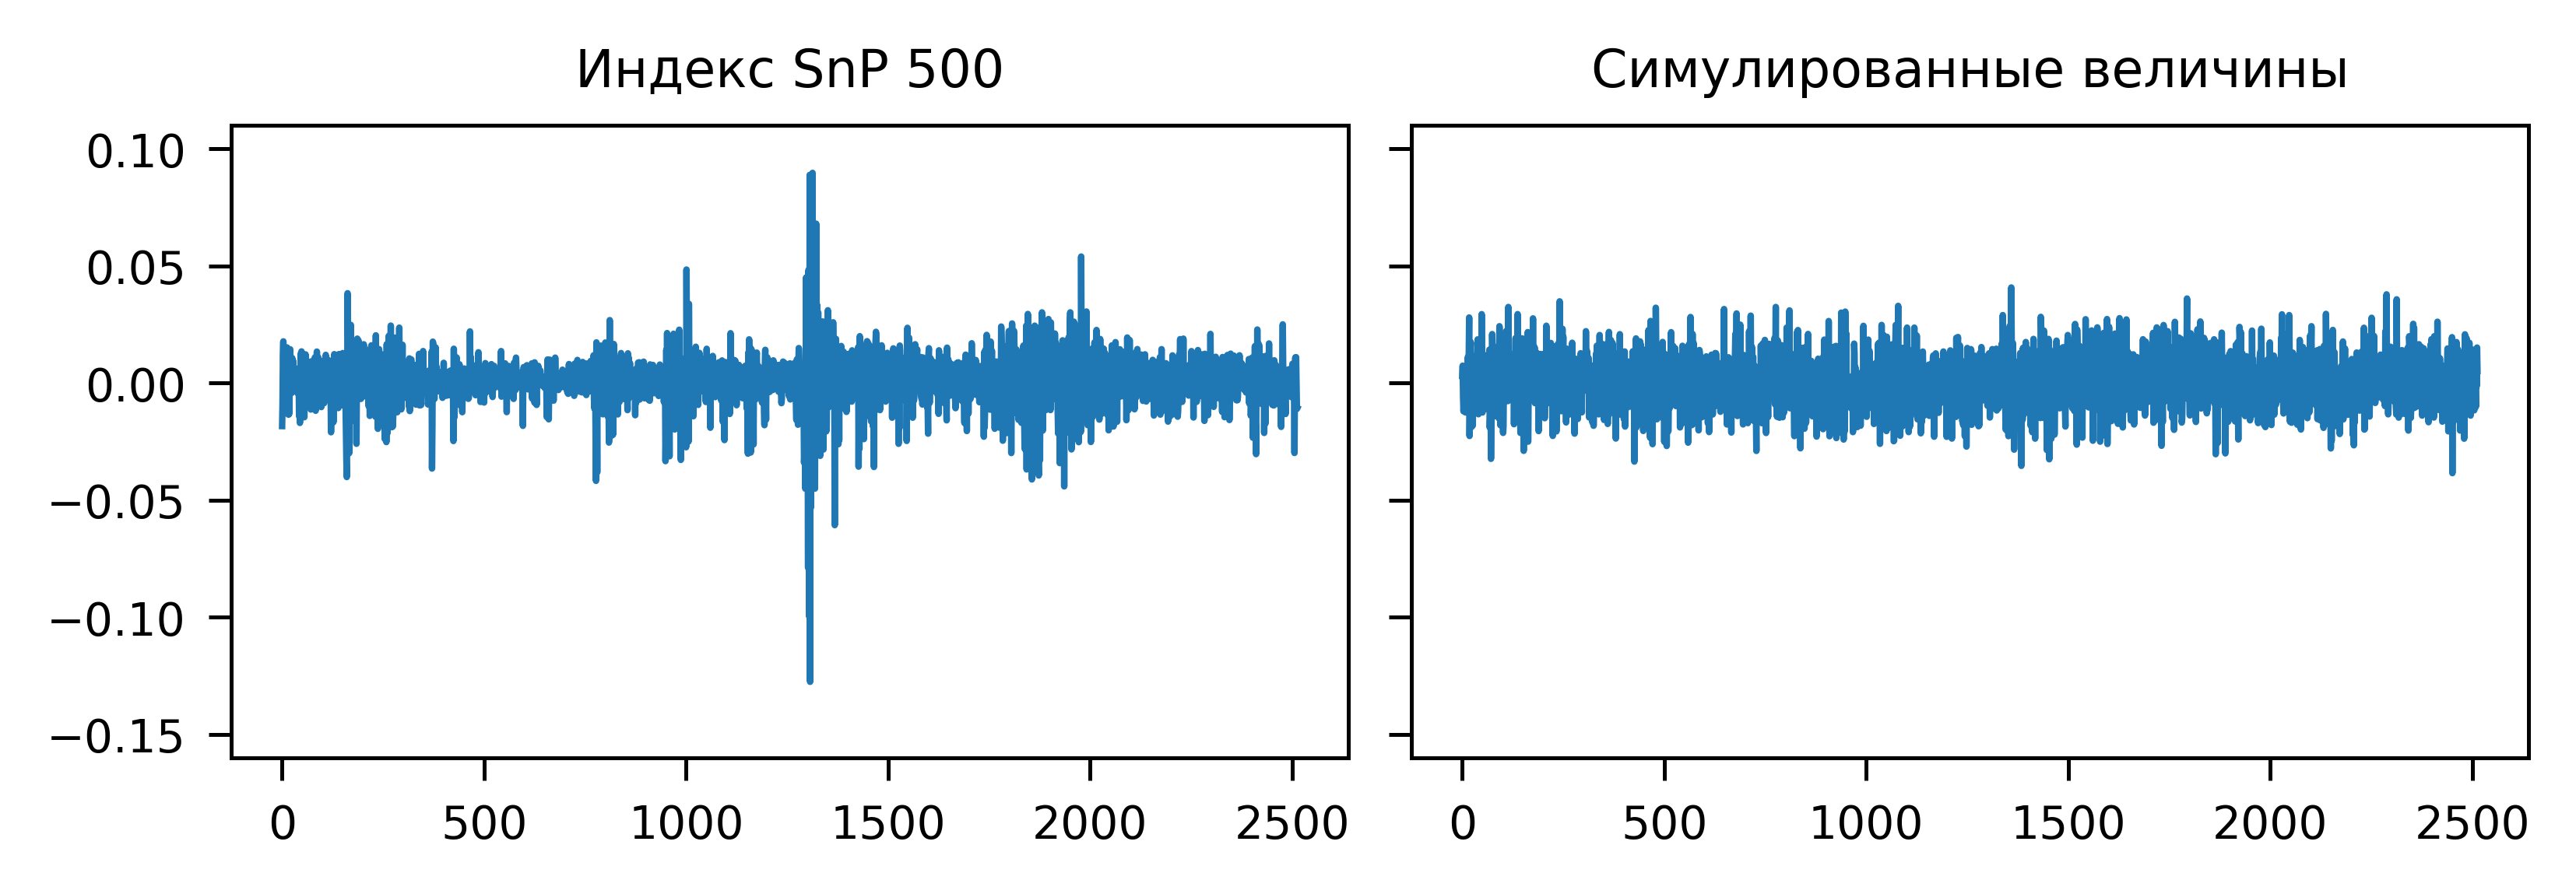
\includegraphics{pic/snp-returns.png}
\centering
\caption{Приращения логарифмов значений индекса SnP 500 и симулированные нормальные случайные величины с такими же средним и дисперсией.}
\label{intro:f:real-vol}
\end{figure}

\begin{figure}[t]
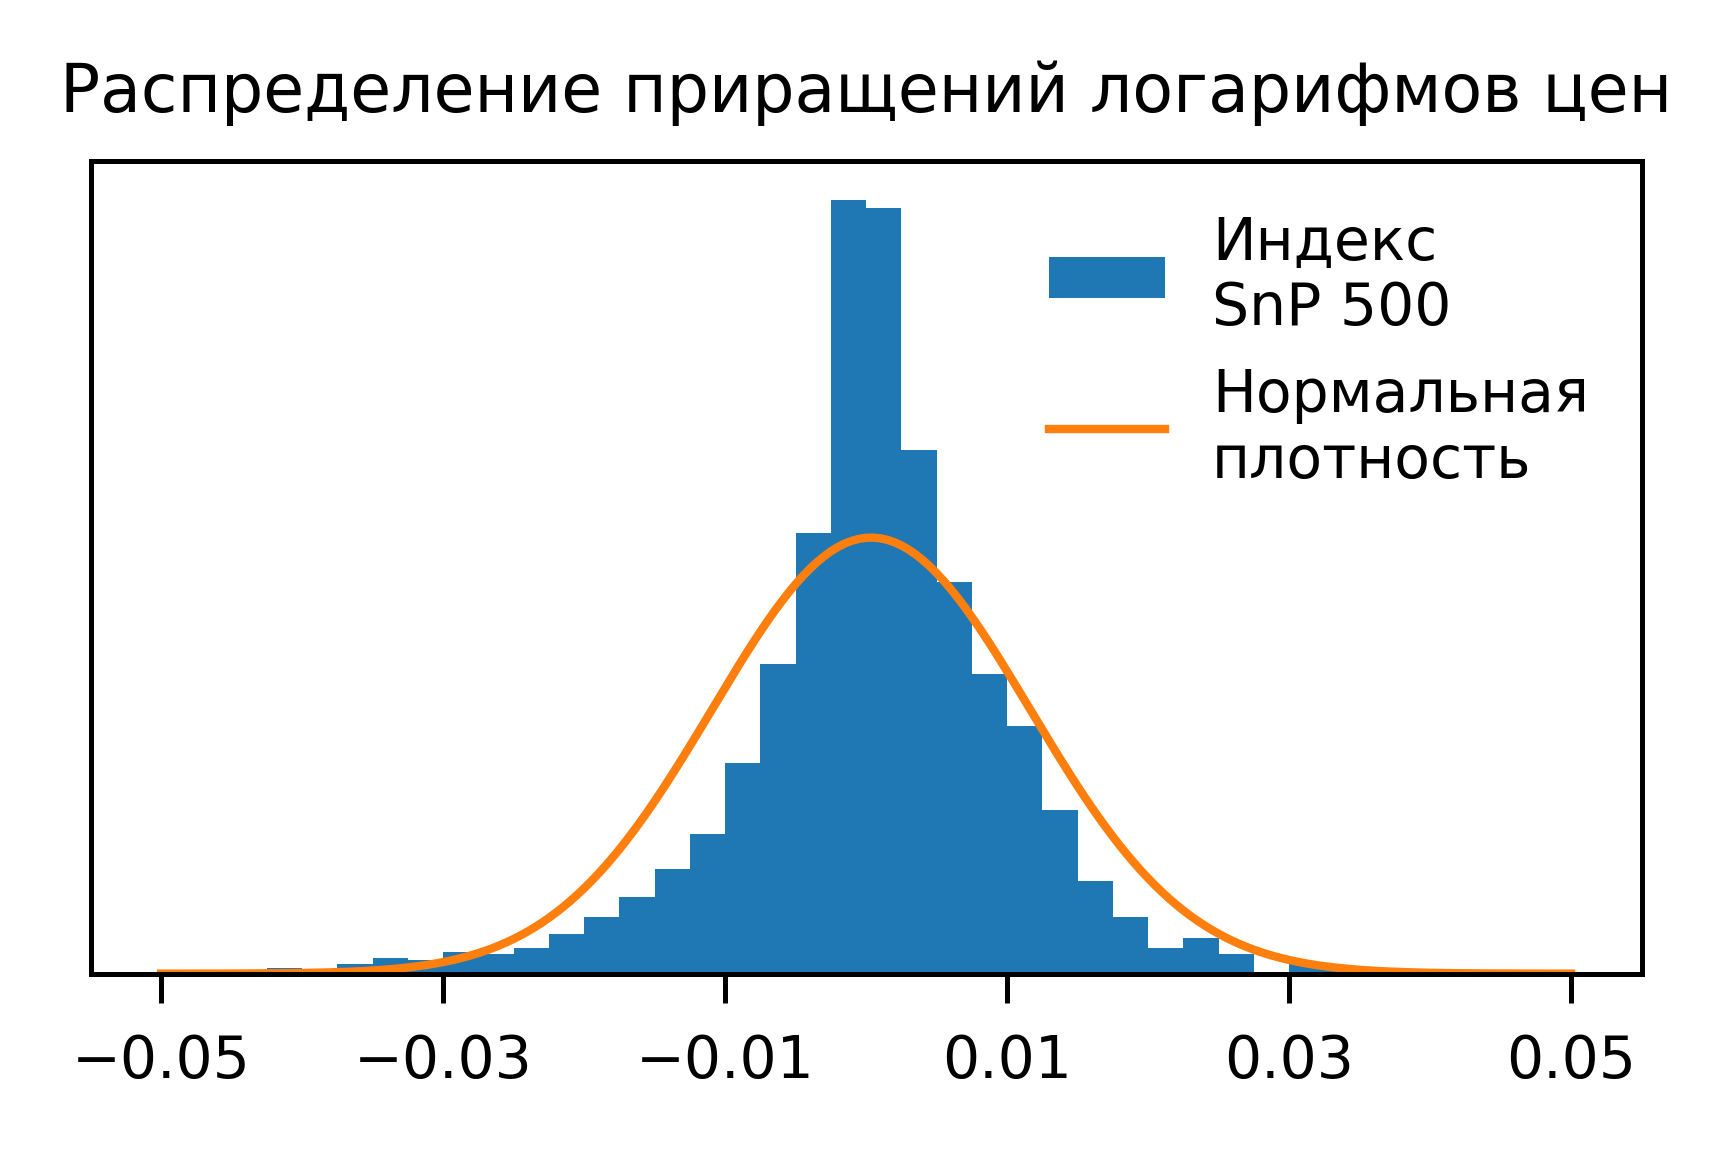
\includegraphics{pic/snp-hist.png}
\centering
\caption{Сравнение эмпирического распределения приращений логарифмов индекса SnP 500 с нормальным распределением.}
\label{intro:f:hist}
\end{figure}


\subsubsection{Автокорреляция}

Для геометрического броуновского движения величины $L_{t+s}$ и $L_t$ независимыми при $s\ge \Delta t$ в силу независимости приращений броуновского движения.
Из независимости следует некоррелированность, поэтому можно вычислить эмпирические коэффициенты корреляции (\te\ автокорреляционную функцию) и посмотреть, близки ли они к нулю.
Оказывается, что для рыночных данных корреляции $\rho(L_{t+s},L_t)$ близки к нулю, но корреляции квадратов приращений логарифмов $\rho(L_{t+s}^2,L_t^2)$ отличается от нуля (см.~рис.~\ref{intro:f:autocorr}).
Это говорит о том, что величины $L_{t+s}$ и $L_t$ зависимы, хотя и слабо коррелированны. 

\begin{figure}[t]
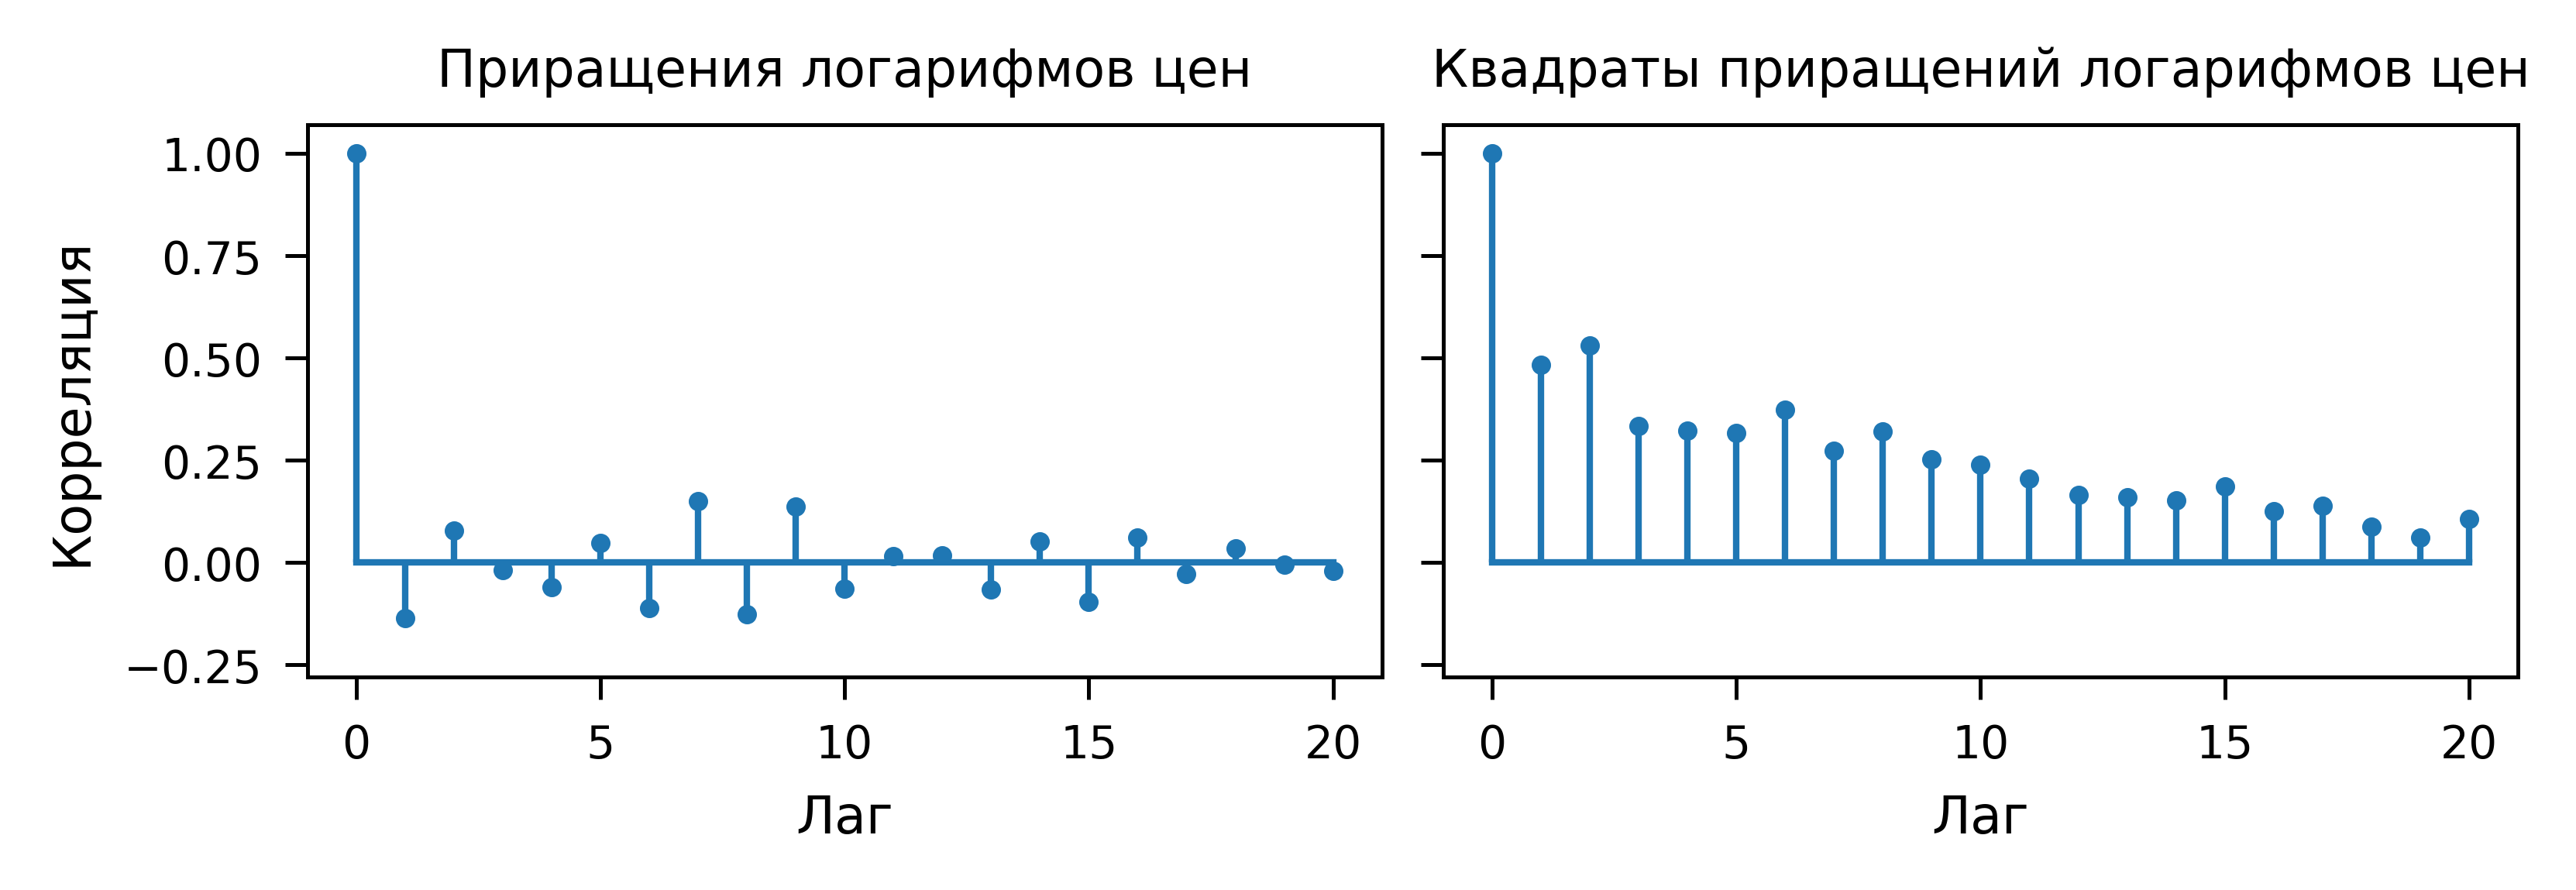
\includegraphics{pic/snp-autocorr.png}
\centering
\caption{Автокорреляционная функция для логарифмов приращений значения индекса SnP 500 и квадратов логарифмов приращений.}
\label{intro:f:autocorr}
\end{figure}


\subsubsection{Другие эмпирические факты}

Обзор статистических свойств рыночных цен приведен в статье \cite{Cont01}.
Эти свойства также называются \emph{стилизованными фактами}.
Кратко перечислим некоторые стилизованные факты, отсылая за подробностями к упомянутой статье.
\begin{itemize}
\item Имеется зависимость между изменениями цены и изменениями волатильности: часто при падении цены волатильность возрастает, а при росте цены остается без существенных изменений или плавно уменьшается. В модели \bs\ такого быть не может, так как величина $\sigma$ постоянна.

\item Кластеризация волатильности: за большими значениями волатильности преимущественно следуют большие значения, за малыми "--- малые.
Если представлять волатильность как степень <<беспокойства>> рынка, то это означает, что на рынке наблюдаются периоды спокойствия и беспокойства.
В модели \bs, напротив, рынок всегда <<одинаково спокоен>>.

\item Присутствие <<скачков>> (\te\ разрывов) в процессах цен, которые нельзя объяснить только тем, что данные собираются дискретным образом.%
\footnote{В этом курсе мы будем рассматривать модели, в которых процессы цен непрерывны.
Модели со скачками, основанные на \emph{процессах Леви}, были популярны в 2000-x гг.}
\end{itemize}


\subsection{Подразумеваемая волатильность}

На ликвидных рынках цены опционов можно считать известными (из рыночных данных), и тогда для каждого опциона можно найти значение $\sigma$ такое, что цена, вычисленная по формуле \bs, совпадает с рыночной ценой "--- это значение $\sigma$ называется \emph{подразумеваемой волатильностью}.
Мы будем обозначать его как $\hat\sigma(T,K)$, когда нужно подчеркнуть зависимость от страйка и времени исполнения.

Если бы рыночные данные следователи модели \bs, то построенная по ним функция $\hat\sigma(T,K)$ была бы постоянной и равнялась параметру волатильности в модели.
В реальности это не так.
Например, на рис.~\ref{intro:f:smiles} приведены \emph{улыбки волатильности}%
\footnote{Улыбкой волатильности называется функция $\hat\sigma(T,K)$, рассматриваемая как функция от страйка $K$ с фиксированным значением $T$.}
для опционов на индекс S\&P 500 с разными датами исполнения.
Видно, что функция $\hat\sigma(T,K)$ не постоянна как по $K$, так и по $T$.

Это приводит к трудности выбора параметра волатильности в модели \bs\ для оценки экзотических производных инструментов.
Например, следует ли для оценки барьерного опциона взять подразумеваемую волатильность, соответствующую страйку, равному барьеру, или страйку, равному текущей цене базового актива?
Хотелось бы иметь модель, которая позволяет оценивать деривативы, без изменения ее параметров под каждый инструмент.

\begin{figure}[t]
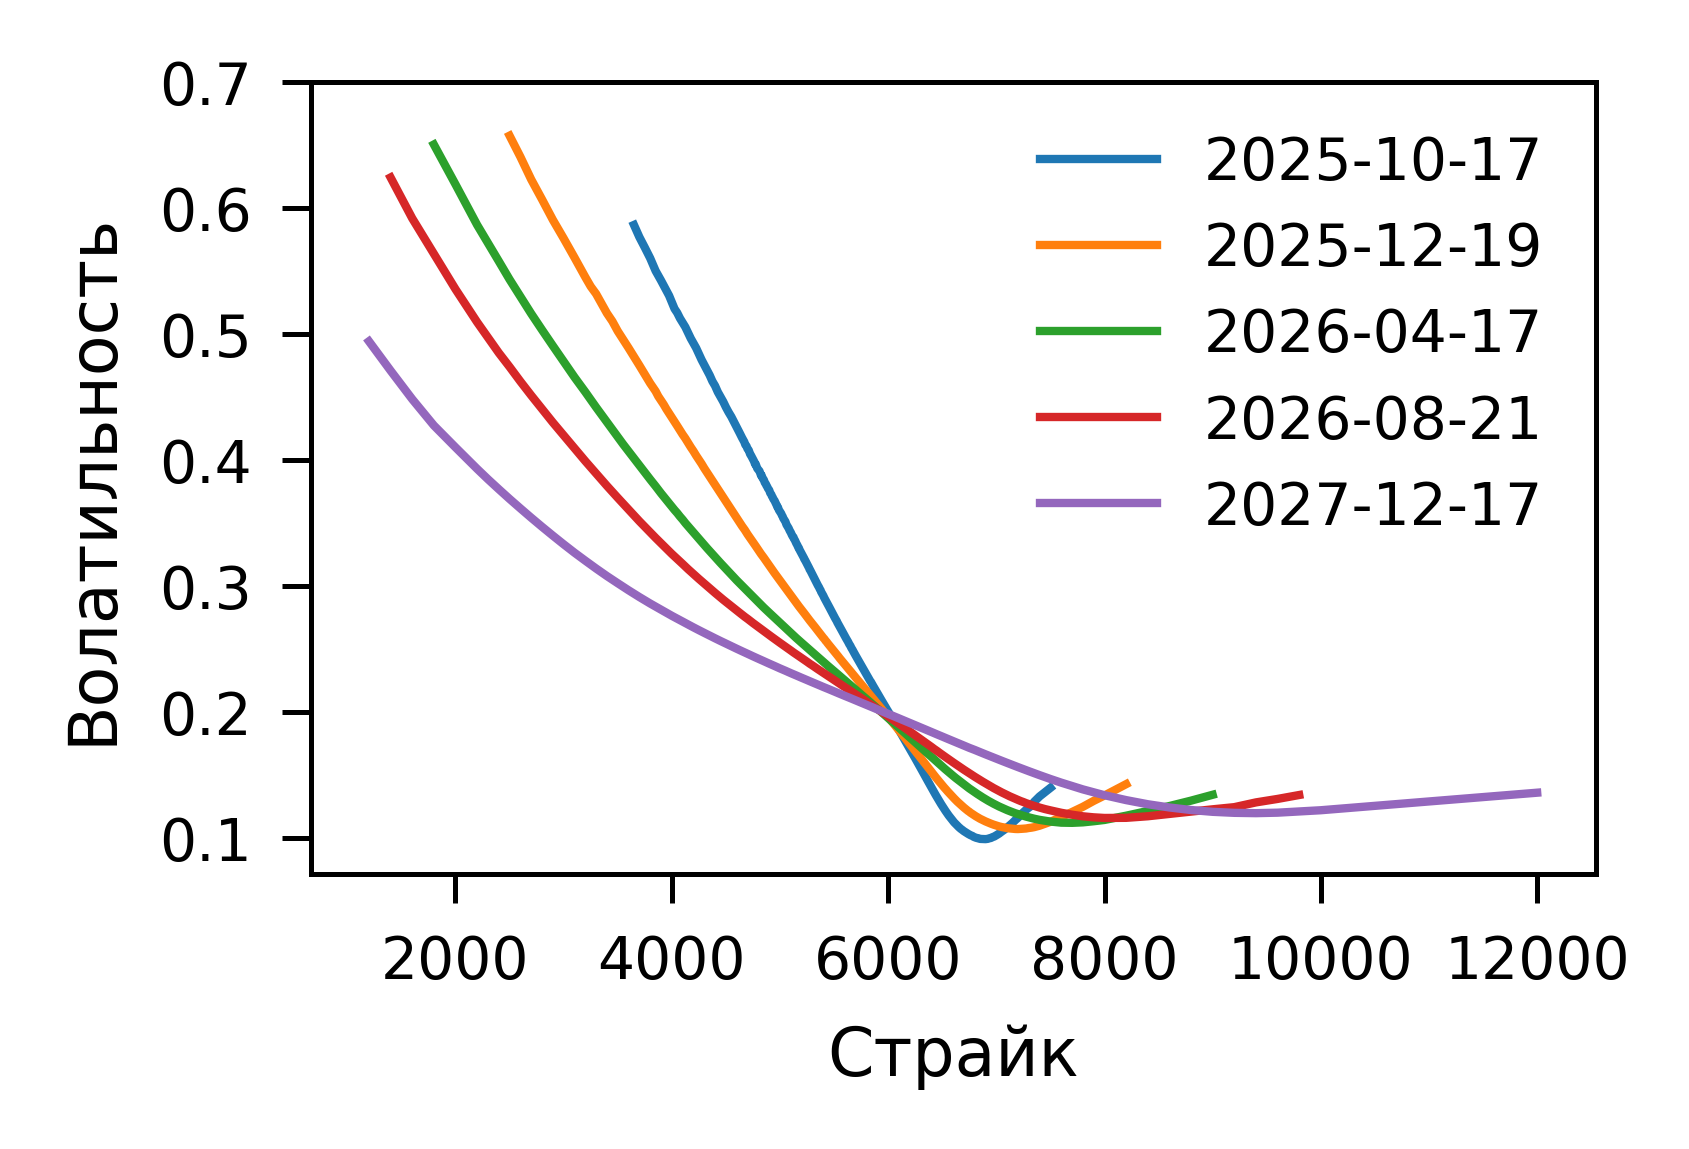
\includegraphics[height=5cm]{pic/snp-smiles.png}
\centering
\caption{Улыбки волатильности для индекса SnP 500 с разными датами исполнения, построенные по ценам опционов на дату  25.04.2024.}
\label{intro:f:smiles}
\end{figure}


\subsection{К каким ошибкам приводит модель \bs?}

Рассмотрим два типа ошибок, свойственных всем моделям и, в том числе, модели \bs.
Естественно, чем ошибка в модели меньше, тем модель лучше.
Соответственно, целью исследования более сложных моделей цен является, в том числе, нахождение моделей дающих меньшие ошибки.

\subsubsection{Статическая ошибка}
Под \emph{статической ошибкой} модели мы будем понимать несоответствие между рыночными ценами ликвидных (т.е.\ активно торгующихся и имеющих доступные рыночные цены) производных инструментов%
\footnote{Под ликвидными производными инструментами далее, в основном, имеются ввиду ванильные европейские опционы колл и пут.}
и ценами этих инструментов, получаемых в модели.

Статическая ошибка приводит к следующему нежелательному эффекту: модель дает цены инструментов, по которым их невозможно купить или продать.
Отметим, что статическая ошибка означает не то, что параметры модели неправильно откалиброваны к рыночным данным, а то, что модель в принципе не способна попасть в набор цен деривативов ни при каких комбинациях своих параметров.

В модели \bs\ статическая ошибка возникает из-за того, что в ней предполагается постоянство волатильности:
каким бы ни был параметр $\sigma$, модель не может воспроизвести рыночные улыбки волатильности, что означает невозможность воспроизвести рыночные цены ванильных опционов.


\subsubsection{Динамическая ошибка}

Под \emph{динамической ошибкой} мы будем понимать несоответствие между вероятностными распределениями процессов цен базовых активов, процессов цен ликвидных производных инструментов, а также других динамических характеристик%
\footnote{Например, такими характеристиками могут быть величины, вычисляемые из поверхности волатильности: волатильность опционов ATM, наклон и кривизна поверхности, и др.}, которые получаются в модели и наблюдаются в реальных данных. 

Динамическая ошибка приводит к ошибке репликации: производные инструменты, которые в выбранной модели теоретически можно реплицировать с помощью самофинансируемых стратегий, не реплицируются в точности.

Поясним на примере.
Пусть требуется реплицировать платежное обязательство, производящее выплату $X$ в момент времени $T$.
Для простоты предположим, что процентная ставка равна нулю, а $X$ зависит только от $S_T$, \te\ $X=f(S_T)$.
Если использовать для репликации модель \bs, то количество рискового актива $H_t$ в реплицируемом портфеле $\pi_t$ должно быть равно дельте инструмента:
\[
H_t = V'_s(t,S_t),
\]
где $V_t(t,s) = \E^{\Q} (f(S_T) \mid S_t=s)$ "--- его цена в модели \bs.
Тогда стоимость портфеля $\pi_t$ в момент исполнения будет равна
\[
V_T^\pi = V(0,S_0) + \int_0^T H_t d S_t = V(0,S_0) + \int_0^T V'_s(t,S_t) d S_t.
\]
С другой стороны, по формуле Ито имеем
\[
V(T,S_T) = V(0,S_0) + \int_0^T V'_t(t,S_t) dt + \int_0^T V'_s(t,S_t) d S_t + \frac12 \int_0^t V''_{ss}(t,S_t) (dS_t)^2.
\]
Так как $X=V(T,S_T)$, то для \emph{ошибки репликации} $\epsilon := V_T^\pi - X$ получаем выражение
\[
\epsilon = \int_0^T V'_t(t,S_t) dt + \frac12 \int_0^t V''_{ss}(t,S_t) (dS_t)^2.
\]

Далее воспользуемся тем, что $V'_t(t,s) = -\frac12 \sigma^2 V''_{ss}(t,s)$, как следует из уравнения \bs\ (при нулевой безрисковой ставке); здесь $\sigma$ "--- параметр волатильности в модели, используемой для репликации.
Если же допустить, что в реальности процесс цены $S_t$ имеет стохастическую волатильность, \te\ $dS_t = \sigma_t S_t d W_t$ со случайным процессом $\sigma_t$, то получим ненулевую ошибку:
\[
\epsilon = \frac12 \int_0^T (\sigma_t^2 - \sigma^2) V''_{ss}(t,S_t)S_t^2 dt.
\]

%%%%%%%%%%%%%%%%%%%%
% Старый фрагмент, непонятно написан
%%%%%%%%%%%%%%%%%%%%
% Рассмотрим функцию $V(t,S_t)$ такую, что $V(T,s) = g(s)$ (пусть пока $V$ произвольна, потом будет видно, как она связана с ценой платежного обязательства).
% Тогда портфель, состоящих из безрискового и рискового актива, стоимость которого в каждый момент времени равна $V(t,S_t)$, реплицирует $X$.
% Будем считать, что портфель не обязательно является самофинансируемым, и величина притока/оттока капитала описывается дифференциалом $C_t dt$.
% Тогда необходимо, чтобы было выполнено равенство $d V(t,S_t) = h_tdS_t + C_t dt$, где $h_t$ "--- количество единиц рискового актива в портфеле. По формуле Ито это эквивалентно равенству
% \[
% C_t dt = V'_t(t,S_t) dt + V'_s(t,S_t) dS_t + \frac12 V''_{ss}(t,S_t) (dS_t)^2 - h_t d S_t.
% \]
% Если выбрать $h_t=V'_s(t,S_t)$, то слагаемые с $dS_t$ сократятся, что уберет зависимость от изменения цены базового актива с точностью до первого порядка (<<дельта-хеджирование>>).
% Подставляя $(dS_t)^2 = \sigma^2 S_t^2 dt$, получаем
% \[
% C_t dt = \left(V'_t(t,S_t) + \frac{\sigma^2}2 V''_{ss}(t,S_t)S_t^2\right) dt.
% \]
% В модели \bs\ величина $\sigma$ постоянна.
% Поэтому, если предполагать, что модель верна, то можно найти функцию $V$ из уравнения в частных производных 
% \begin{equation}
% \label{intro:v}  
% V'_t + \frac{\sigma^2}{2} V''_{ss} = 0
% \end{equation}
% с терминальным условием $V(T,s) = f(s)$, что даст нулевой приток капитала $C_t$, и, таким образом, получится самофинансируемый портфель, который реплицирует $X$.

% Если же допустить, что волатильность $\sigma$ не постоянна, то получим (по-прежнему считая, что $V$ удовлетворяет \eqref{intro:v})
% \[
% C_t = \frac{\sigma_t^2-\hat\sigma^2}{2} V''_{ss}(t,S_t) S_t^2, 
% \]
% где $\hat\sigma$ "--- значение волатильности, которое использовалось при решении уравнения \eqref{intro:v}.
% Таким образом, денежная величина ошибки хеджирования составит
% \[
% C_T = \int_0^T \frac{\sigma_t^2-\hat\sigma^2}{2} V''_{ss}(t,S_t) S_t^2 dt.
% \]
% Тот факт, что $C_T$ не равно нулю означает наличие ошибки репликации.
% Она здесь возникла из-за того, что в модели предполагается постоянство коэффициента $\sigma$, а в реальности $\sigma_t$ не постоянно.
%%%%%%%%%%%%%%%%%%%%

\section{Краткая история моделей стохастической волатильности}

Под моделями стохастической волатильности мы будем понимать модели, в которых процесс цены базового актива относительно эквивалентной мартингальной меры имеет вид
\[
dS_t = r_tS_t dt + \sigma_t S_t dW_t,
\]
где $r_t$ "--- безрисковая процентная ставка (в этом курсе она будет, как правило, считаться детерминированной функцией), a $\sigma_t$ "--- случайный процесс\footnote{В случае, когда $\sigma_t$ является функцией только от текущего значения цены $S_t$ и времени, волатильность часто называют \emph{локальной}, а не стохастической; см.~далее.}.
Замена постоянного параметра $\sigma$ в модели \bs\ на случайный процесс приводит к большому разнообразию получаемых моделей. 

Далее перечислим некоторые известные модели стохастической волатильности, кратко упомянув их достоинства и недостатки.
При первом чтении этого раздела многое может показаться непонятным.
К нему стоит вернуться после окончания курса.

\subsubsection{Модель CEV}

Первой моделью стохастической волатильности была \emph{модель CEV}\footnote{Constant Elasticity of Variance "--- модель c постоянной эластичностью дисперсии.}, предложенная Дж.~Коксом (J.~Cox, 1975).
Уравнение цены в ней имеет вид
\[
d S_t = r_tS_t dt + \sigma S_t^\gamma d W_t,
\]
где $\gamma \ge 0$ и $\sigma>0$ "--- параметры модели. Таким образом, здесь $\sigma_t = \sigma S_t^{\gamma-1}$. 
При $\gamma=1$ получается модель \bs, а при $\gamma=0$ "--- модель Башелье.

Если $\gamma\in[0,1)$, то волатильность растет, когда цена падает, и падает, когда, цена растет.
В первом приближении такое поведение действительно наблюдается в ценах акций.
Кроме того, улыбки волатильности в модели CEV при $\gamma\in(0,1)$ получаются скошенными вправо, что тоже в некоторой степени соответствует наблюдаемым данным.
Если $\gamma>1$, то получается противоположное поведение, которое не характерно для рынков акций, но, может наблюдаться, например, на рынках товаров.

У модели CEV имеется два недостатка.
Во-первых, она недостаточно гибкая, чтобы правильно описывать наблюдаемые поверхности подразумеваемой волатильности (у нее всего два параметра).

Во-вторых, функциональная зависимость $\sigma_t=\sigma(S_t)$ означает, что волатильность зависит только от текущего уровня цены, но в реальности на изменение волатильности оказывают влияние и другие факторы.
Можно провести такой мысленный эксперимент.
Пусть сегодня акция стоит 100, а через год будет стоить 120.
Если за этот год цена акции будет расти <<равномерно>> то можно ожидать, что к концу года волатильность будет в пределах своих <<обычных>> значений.
Однако, если за первые 11 месяцев цена вырастет до 180, а за последний месяц упадет до 120, то волатильность будет высокой. 
В модели CEV, напротив, в обоих случаях волатильность должна быть одинаковой.


\subsubsection{Модель локальной волатильности}

Модель локальной волатильности, предложенная Б.~Дюпиром (B.~Dupire, 1994), решает проблему статической ошибки: она в точности калибруется к ценам наблюдаемых европейских опционов.
Модель имеет вид
\[
d S_t = r_tS_t dt + \sigma(t,S_t) d W_t,
\]
где $\sigma(t,s)$ "--- детерминированная функция, которая определяется из рыночных цен опционов по некоторой аналитической формуле.

Несмотря на отсутствие статической ошибки, в модели локальной волатильности присутствует динамическая ошибка по той же причине, что и в модели CEV "--- из-за жесткой связи волатильности и цены.


\subsubsection{Модель Хестона}
Одной из наиболее известных моделей стохастической волатильности является модель C.~Хестона (S.~Heston, 1993).
Она задается уравнениями
\begin{align*}
&d S_t = r_tS_tdt + \sqrt{V_t} d W_t^{(1)},\\
&d V_t = \kappa(\theta - V_t)dt + \sigma \sqrt{V_t} d W_t^{(2)},\\
&d W_t^{(1)} d W_t^{(2)} = \rho dt,
\end{align*}
где процесс $V_t$ называется стохастической дисперсией (а $\sigma_t = \sqrt{V_t}$ "--- стохастической волатильностью).
Величины $\kappa,\theta,\sigma,\rho, V_0$ "--- параметры модели.
Третье уравнение означает, что броуновские движения $W_t^{(1)}$ и $W_t^{(2)}$ являются коррелированными с коэффициентом корреляции $\rho$ (\te\ $\E W_t^{(1)}W_t^{(2)} = \rho t$).

Пять параметров придают модели Хестона достаточно гибкости в подгонке к рыночным ценам опционов, но она все равно имеет статическую ошибку "--- это неизбежно при конечном числе параметров.
С другой стороны, зависимость волатильности от дополнительного случайного фактора позволяет более правильно отражать ее динамику по сравнению с моделью локальной волатильности. 

Большим достоинством модели Хестона является наличие эффективного способа вычисления цен европейских опционов, что необходимо для калибровки параметров модели.
Это важное свойство любой модели "--- можно придумать много разных уравнений, задающих стохастическую волатильность, но если нет эффективного метода вычисления цен простых деривативов, то такую модель модель будет трудно использовать на практике.

%%%%%%%%%%%%%%%%%%%%
%%% Непонятный абзац
%%%%%%%%%%%%%%%%%%%%
% Из недостатков модели Хестона можно отметить то, что она является недостаточно гибкой для описания динамики поверхности подразумеваемой волатильности.
% А именно, если откалибровать параметры модели по наблюдаемой поверхности подразумеваемой волатильности в текущий момент времени, то эти параметры будут также определять вероятностное распределение того, как вся поверхность будет двигаться в последующие моменты времени: грубо говоря, получается, что начальное значение процесса жестко связано с его распределением.
% Хотелось бы иметь параметры, которые будут отдельно контролировать динамику волатильности.
% Это необходимо для оценки экзотических деривативов, которые зависят от будущих значений волатильности (например, опционов с форвардным стартом). 

В дополнение к модели Хестона упомянем некоторые другие модели, в которых волатильность задается диффузионным процессом; эти модели не будут рассматриваться с нашем курсе, но они довольно обширно изучались в литературе: модель Халла"--~Уайта (Hull"--~White), модель Стейна"--~Стейна (Stein"--~Stein), модель 3/2.


\subsubsection{Модель SABR}

Другой хорошо известной моделью стохастической волатильности является модель SABR\footnote{Stochastic Alpha, Beta, Rho "--- стохастическая альфа, бета, ро.}, предложенная П.~Хэганом  соавторами (P.~Hagan, D.~Kumar, A.~Lesniewski, D.~Woodward, 2002):
\begin{align*}
&d S_t = r_t S_t dt + \alpha_t F_t^\beta d W_t^{(1)},\\
&d\alpha_t = \nu\alpha_t d W_t^{(2)},\\
&d W_t^{(1)} d W_t^{(2)} = \rho dt,
\end{align*}
где $\alpha_0,\beta,\nu,\rho$ "--- параметры модели.

Достоинство модели SABR состоит в том, что для нее имеется приближенная аналитическая формула для подразумеваемой волатильности, которая  позволяет быстро калибровать параметры модели и вычислять цены ванильных опционов.

Вообще, модель SABR часто используется не как динамическая модель, а именно как формула для интерполяции улыбок волатильности с учетом их динамики при изменении цены базового актива.
Под интерполяцией понимается то, что в реальности значения подразумеваемой волатильности даны в дискретном наборе точек (для разных страйков времен исполнения).

Поясним на примере.
Пусть $V(t,s,\sigma)$ "--- функция, задающая цену опциона по формуле \bs.
Чтобы получить его рыночную цену, вместо $\sigma$ нужно подставить подразумеваемую волатильность $\hat\sigma(t,s)$ этого опциона%
\footnote{Здесь параметры опциона $T,K$ фиксированы, но считается, что подразумеваемая волатильность зависит от времени и цены базового актива.
Может присутствовать зависимость и от других факторов, но для простоты мы сейчас ей пренебрежем.}.
Тогда, например, дельта опциона будет вычисляться как
\[
\Delta = \prt {V}s + \prt {V}\sigma \prt{\hat\sigma} s = \Delta_{BS} + \mathcal{V}_{BS} \prt{\hat\sigma} s,
\]
где $\Delta_{BS}$ и $\mathcal{V}_{BS}$ "--- дельта и вега в модели \bs.
Таким образом, возникает поправка в виде последнего члена, связанная с тем, что улыбка волатильности обладает динамикой (движется при изменении цены $s$).
Имея аналитическую формулу для $\hat\sigma$, эту поправку легко вычислить. 


\subsubsection{Модель SVI}

Модель SVI\footnote{Stochastic Volatility Inspired "--- модель, <<вдохновленная>> стохастической волатильностью.} (J. Gatheral, 1999) "--- это метод интерполяции и экстраполяции улыбок волатильности.
Она представляет из себя специально подобранную аналитическую функцию, зависящую от 5 параметров, которая хорошо <<ложится>> на рыночные улыбки волатильности.%
\footnote{Модель SVI не описывает динамику движения цен, \te, в общем-то, не является моделью стохастической волатильности.}

Задача интерполяции и экстраполяции волатильности является непростой по той причине, что желательно интерполировать и экстраполировать так, чтобы цены ванильных опционов, вычисленные по получаемой подразумеваемой волатильности, не приводили к наличию арбитража. 
При использовании общих методов (таких, как например, сплайны), добиться этого труднее, чем при использовании SVI.


\subsubsection{Модель Бергоми}

Модель Бергоми (L.~Bergomi, 2004--2005) позволяет более аккуратно моделировать динамику форвардной дисперсии, что важно для оценки экзотических опционов, зависящих от значений подразумеваемой волатильности в будущем.

В общем случае модель Бергоми порождается $n$ броуновскими движениями ($n$-факторная модель), но сейчас для простоты рассмотрим только ее 1-факторную версию.
Она задается уравнениями
\begin{align*}
&d S_t = r_tS_t dt + \sqrt{\xi_t^t} S_t d W_t^{(1)},\\
&d \xi_t^T = \omega e^{-k(T-t)} \xi_t^T d W_t^{(2)}, \quad T>0,\ t\in [0,T],\\
&dW_t^{(1)}dW_t^{(2)} = \rho dt.
\end{align*}
где $\omega,\kappa,\rho$ "--- параметры модели, а $\xi^T = (\xi_t^T)_{t\in[0,T]}$ "--- семейство процессов \emph{$T$"=форвардной дисперсии}, индексированных параметром $T>0$, задающим дату экспирации.

Под $T$-форвардной дисперсией на дату $t$ понимается случайная величина $\xi_t^T = \E^{\Q}(\sigma_T^2 \mid \F_t)$, \te\ условное ожидание квадрата стохастической волатильности в будущем. Для каждого $T$ получается свой процесс $\xi^T_t$ с временем $t\le T$. 
Если зафиксировать текущее время $t$, то получится кривая форвардной дисперсии $\xi_t^T$, $T\ge t$. 
Мгновенная стохастическая волатильность равна $\sigma_t = \sqrt{\xi_t^t}$.

Начальная кривая форвардной дисперсии $\xi^0$ является параметром модели и может быть оценена по рыночным данным.
Несмотря на то, что в каждый момент времени $t$ имеется континуум значений форвардной дисперсии $\xi_t^T$, $T\ge t$, вся кривая управляется всего одним броуновским движением $W_t$ (в $n$-факторной модели будет $n$ броуновских движений), что делает модель доступной для аналитических и численных расчетов.


\subsubsection{Модели грубой волатильности}

В 2010-x гг.\ в научной литературе получили популярность модели, где стохастическая волатильность задается процессами, которые имеет более хаотичные (грубые) траектории, чем диффузионные процессы.
Примером такой модели является
\begin{align*}
&d S_t = r_tS_t dt + \sigma_t S_t d W_t,\\
&\sigma_t = \sigma e^{\nu W_t^H}
\end{align*}
где $W_t^H = (W_t^H)_{t\ge0}$ "--- \emph{дробное} (или, еще говорят, \emph{фрактальное}) броуновское движение с параметром $H\in(0,1)$.
По определению, дробным броуновским движением называется гауссовский случайный процесс с нулевым средним и ковариационной функцией $\cov(W_t^H,W_s^H) = \frac12 (t^{2H} + s^{2H} - |t-s|^{2H}) $.
При $H=1/2$ получается стандартное броуновское движение.
С помощью параметра $H$ можно контролировать грубость траекторий: чем $H$ ближе к нулю, тем траектории грубее%
\footnote{Более точно: на любом конечном отрезке траектории процесса $W^H$ с вероятностью 1 непрерывны по Гёльдеру с показателем $H'$ для любого $H' < H$.}.

К идее грубой волатильности приводят два наблюдения.
Во-первых, статистический анализ внутридневных изменений цен показывает, что распределение реализованной волатильности за день обладает свойствами, которые не могут получиться у диффузионных процессов, но ими обладает, например, фрактальное геометрическое броуновское движение с малым показателем $H$ (со значением примерно $H=0.15$).
Во-вторых, в рыночных поверхностях подразумеваемой волатильности наблюдается такой эффект, что коэффициент наклона улыбки волатильности ведет себя примерно как $T^p$ при времени до исполнения $T$ близком к нулю, где значение показателя $p$ близко к $-1/2$.
Опять же, этого нельзя достичь в моделях, где волатильность задается диффузионным процессов, но можно, если она более грубая.

В литературе изучались разные модификации стандартных моделей на случай грубой волатильности: грубая модель Хестона, грубая модель SABR, грубая модель Бергоми и \tp\ 
Большим недостатком моделей грубой волатильности является сложность работы с ними аналитически и численно.
Это вызвано тем, что дробное броуновское движение не является ни марковским процессом, ни семимартингалом (за исключением случая $H=1/2$), и поэтому стандартные средства из стохастического анализа к нему не применимы.
К настоящему время в финансовой индустрии модели грубой волатильности так и не начали активно использоваться.


\subsubsection{Модели локальной стохастической волатильности}

Локальная стохастическая волатильность "--- это <<надстройка>> над какой"=либо моделью стохастической волатильности, заключающаяся в добавлении в коэффициент волатильности\emph{ функции левериджа $\ell(t,s)$}:
\[
d S_t = r_tS_t dt + \sigma_tS_t\ell(t,S_t) dW_t,
\]
где $\sigma_t$ "--- стохастическая волатильность, заданная конкретным процессом, зависящим от парамеров (например, как в модели Хестона, Бергоми и \tp), а функция левериджа $\ell(t,s)$ подбирается таким образом, чтобы исключить статическую ошибку.
Стохастическая часть модели (процесс $\sigma_t$) дает <<правильные>> динамические характеристики, а локальная часть (функция $\ell$) "--- статические.

Из результатов для модели локальной волатильности выводится, что $\ell$ выражается через условное математическое ожидание $\E(\sigma_t\mid S_t)$, что приводит к уравнению
\begin{equation}
\label{intro:lsv}
dS_t = rS_t dt + \sigma_t S_t f(t,S_t,\E(\sigma_t\mid S_t)) d W_t,
\end{equation}
где функция $f$ выписывается явно через поверхность локальной волатильности.
Это уравнение представляет собой стохастическое дифференциальное уравнение Маккина"--~Власова, \te\ уравнение в котором коэффициенты зависят от вероятностного распределения его решения.

Модели локальной стохастической волатильности являются современным <<стандартом>> в финансовой индустрии, особенно в задачах оценки деривативов, зависящих от нескольких базовых активов. 
Определенную трудность при работе с ними представляет калибровка локальной части, \te\ численное нахождение функции $\ell(t,s)$.
Более того, в настоящее время до конца не понятно, при каких условиях уравнение \eqref{intro:lsv} корректно задает модель, \te\ когда у него существует единственное решение, а также при каких условиях используемые численные методы сходятся к теоретическому решению. 


\summary
\begin{itemize}
\item Модель \bs\ неправильно описывает вероятностные распределения цен: в реальности приращения их логарифмов имеют распределение, отличное от нормального, обладают тяжелыми хвостами и зависимы.
\item Модель \bs\ также неправильно описывает поверхности подразумеваемой волатильности: в ней они плоские, а в реальности это не так.
\item Моделям присущи статические и динамические ошибки.
Первая означает несоответствие между рыночными ценами ликвидных производных инструментов и ценами этих инструментов в модели; вторая "--- несоответствие между вероятностными распределениями процессов цен базовых и производных инструментов, которые получаются в модели и наблюдаются в реальных данных. 
\end{itemize}

%!TEX root=finmath2.tex

\chapter{Фундаментальные результаты}
\label{ch:general}
\chaptertoc

Эта лекция посвящена фундаментальным теоретическим результатам.
Основная ее цель "--- показать, как определить справедливую цену платежного обязательства, и объяснить, почему ее можно вычислить в виде ожидания дисконтированной выплаты по эквивалентной мартингальной мере.


\section{Общая модель рынка}

Пусть дано фильтрованное вероятностное пространство $(\Omega,\F,(\F_t)_{t\in[0,T]},\P)$ со стандартным $d$-мерным броуновским движением $W_t=(W_t^1,\dots,W_t^d)$. 
Горизонт времени $T$ конечен.

Рынок в модели состоит из одного безрискового актива и $N$ рисковых активов.
Цена безрискового актива задается процессом
\[
d B_t = r_tB_t dt \qquad\Bigl[B_t = B_0 e^{\int_0^t r_s ds}\Bigr].
\] 
Без ограничения общности считается, что $B_0=1$.
В этой лекции процентная ставка $r_t$ случайная, хотя далее в курсе она, как правило, будет детерминированной (но не постоянной по времени).
Всегда будем предполагать, что $r_t$ ограничена снизу, \te\ $r_t\ge\underline r$ для некоторой константы $\underline r$.

Цены рисковых активов задаются процессами Ито
\begin{equation}
\label{gen:risky}
d S_t^n = \mu_t^n dt + \sum_{i=1}^d \sigma^{ni}_t d W_t^i,
\end{equation}
где $\mu_t^n$, $\sigma_t^{ni}$ "--- некоторые случайный процессы, для которых стохастические интегралы в формуле выше корректно определены.\footnote{Отметим, что здесь в коэффициенты сноса и диффузии не входит множитель $S_t$, как, например, в модели \bs.
Это дает большую общность рассуждений.}
Будем считать, что рисковые активы могут выплачивать дивиденды с интенсивностями, задаваемыми случайными процессами $q_t^n\ge0$.

\begin{remark}
Уравнение \eqref{gen:risky} представляет общую форму модели рынка, где цены рисковых активов задаются процессами Ито.
Однако, в дальнейших лекциях мы, в основном, будем иметь дело с моделями, содержащими один рисковый актив с ценой
\begin{equation}
\label{gen:risky-simple}
d S_t^n = \mu_t^n dt + \sigma_t d W_t,
\end{equation}
где $W_t$ "--- одномерное броуновское движение, при этом процесс $\sigma_t$ управляется другим броуновским движением, которое коррелированно с $W_t$.
\end{remark}

\begin{definition}
\label{gen:d:strategies}
\emph{Торговой стратегией} называется измеримый согласованный%
\footnote{В литературе часто считают, что стратегии задаются \emph{предсказуемыми} процессами.
Однако если цены задаются процессами Ито, то модели с согласованными и предсказуемыми стратегиями будут, в сущности, эквивалентны.}
процесс $\pi=(\pi_t)_{t\in[0,T]}$, где $\pi_t=(G_t,H_t^1,\dots,H_t^N)$.
\emph{Стоимостью портфеля} стратегии $\pi$ называется процесс
\[
V_t^\pi = G_tB_t + \sum_{n=1}^N H_t^n S_t^n.
\]
Стратегия $\pi$ называется \emph{самофинансируемой}, если корректно определены интегралы\footnote{Первые два интеграла понимаются как потраекторные интеграла Лебега, а третий интеграл "--- как стохастический интеграл по процессу Ито.
Они корректно определены при выполнении условий
$\int_0^T r_t B_t|G_t| dt < \infty$,
$\int_0^T \bigl(|\mu_t^n H_t^n| + |q_t^n H_t^n|\bigr)dt < \infty$,
$\int_0^T (\sigma_t^{ni} H_t^n)^2 dt < \infty$.}
$\int_0^t G_t d B_t$, $\int_0^t q_t^n H_t^n S_t^n dt$, $\int_0^t H_t^n dS_t^n$ и выполнено равенство (понимаемое в интегральном смысле)
\begin{equation}
\label{gen:sf}
d V_t^\pi = G_t d B_t + \sum_{n=1}^N H_t^n (q_t^n S_t^n dt + d S_t^n).
\end{equation}
Стратегия $\pi$ называется \emph{допустимой}, если существует константа $c$ такая, что $V_t^\pi \ge c$ для всех $t\in[0,T]$.
\end{definition}

Далее под словом <<стратегия>> мы будем всегда понимать допустимую самофинансируемую стратегию, если не оговорено иного.

Определение стоимости портфеля и условие самофинансируемости аналогичны соответствующим определениям, которые были даны для модели \bs\ в курсе <<Введение в финансовую математику>>, поэтому мы не будем подробно останавливаться на их интерпретации.

Что касается допустимости, то в том курсе использовалось более сильное условием (процесс $H_tS_t$ квадратично интегрируем относительно эквивалентной мартингальной меры), которое в общей модели не удобно, так как в ней нет явного выражения для ЭММ.
Напомним, что условие допустимости необходимо, чтобы избежать арбитражных возможностей.

\begin{definition}
\emph{Дисконтированными ценами рисковых активов с учетом дивидендов} называются процессы 
\[
\tilde S_t^n = e^{\int_0^t q_s^n ds}\frac{S_t^n}{B_t} = e^{\int_0^t (q_s^n -r_s)ds}S_t^n.
\]
\emph{Дисконтированной стоимостью} портфеля стратегии $\pi$ называется процесс 
\[
\tilde V_t^\pi = \frac{V_t^\pi}{B_t} = e^{-\int_0^t r_sds} V_t^\pi.
\] 
\end{definition}

% \begin{proposition}
% Стратегия $\pi$ является самофинансируемой тогда и только тогда, когда 
% \begin{equation}
% \label{gen:sf-discounted}
% d\tilde V_t^\pi = \sum_{n=1}^N e^{-\int_0^t q_s^n ds} H_t^nd\tilde S_t^n.
% \end{equation}
% \end{proposition}
% Доказательство этого результата практически повторяет доказательство аналогичного утверждения для модели \bs\ (см.~лекцию 10 во <<Введении в финансовую математику>>), поэтому мы его опустим.


\section{Отсутствие арбитража и безарбитражные цены}

Следующая задача "--- определить, что понимать под справедливой ценой платежного обязательства.
Так как большинство моделей, которые мы будем рассматривать, являются неполными, то понятие цены репликации, которым мы пользовались в модели \bs, здесь не является подходящим. 
Вместо него мы будем пользоваться понятием \emph{безарбитражной} цены.
Для этого сначала обсудим понятие арбитража и условия его отсутствия.


\subsection{Первая фундаментальная теорема финансовой математики}

Напомним, что один из центральных результатов для моделей рынка с дискретным временем "--- \emph{первая фундаментальная теорема} финансовой математики "--- утверждает, что  отсутствие арбитража равносильно существованию эквивалентной мартингальной меры.
В непрерывном времени ситуация становится сложнее, и для того, чтобы получить аналогичный результат, возникает необходимость ввести новые понятия.

% Определение наиболее близкое к статье DS-94
% \begin{definition}
% Будем говорить, что в модели рынка выполнено \emph{условие NFLVR} (no free lunch with vanishing risk "--- отсутствие бесплатного ланча с исчезающим риском) и называть такой рынок \emph{безарбитражным}, если не существует $\F_T$"=измеримой случайной величины $X\in L^\infty$ и последовательности $\F_T$"=измеримых случайных величин $X^n\in L^\infty$ таких, что 
% \begin{alphenum}
% \item $X\ge 0$;
% \item $\P(X>0) > 0$;
% \item $X^n \le V_T^{\pi^n}$ для некоторых стратегий $\pi^n$ c $V_0^{\pi^n} = 0$;
% \item $X^n \to X$ в $L^\infty$ при $n\to\infty$.
% \end{alphenum}
% \end{definition}
% \begin{remark}
% Напомним, что $L^\infty$ "--- это пространство классов эквивалентности существенно ограниченных величин с нормой $\|X\|_{L^\infty} = \inf\{c\in\R : |X| \le c\ \as\}$. 
% \end{remark}

% Эквивалентное, но более простое определение
\begin{definition}
Будем называть $\F_T$-измеримую случайную величину $X$ \emph{бесплатным ланчем с исчезающим риском} (free lunch with vanishing risk, FLVR), если
\begin{alphenum}
\item $X\ge 0$ \as,
\item $\P(X>0)>0$,
\item для любого $\epsilon>0$ найдется стратегия $\pi$ такая, что $V_0^\pi=0$, $V_T^\pi \ge X-\epsilon$ \as
\end{alphenum}

Будем говорить, что в модели рынка выполнено \emph{условие отсутствия бесплатного ланча с исчезающим риском} (no free lunch with vanishing risk, NFLVR) и называть такой рынок \emph{безарбитражным}, если бесплатного ланча с исчезающим риском не существует.
\end{definition}

Смысл условия NFLVR состоит в том, что, начиная из нулевого портфеля, нельзя получить прибыль с риском, стремящемся к нулю (прибыль равна $X$, а <<исчезающий>> риск равен $\epsilon$, который можно выбрать сколь угодно малым).

NFLVR является более сильным условием, чем простое условие отсутствие арбитража (NA).
Напомним, что NA означает, что не существует такой стратегии $\pi$, что $V_0^\pi = 0$, 
$V_T^\pi \ge 0$ и $\P(V_T^\pi > 0) > 0$.
Если NA не выполнено, то $X=V_T^\pi$ и будет бесплатным ланчем с исчезающим риском. 

\begin{definition}
\emph{Эквивалентной локальной мартингальной мерой} (ЭЛММ) называется вероятностная мера $\Q\sim\P$, относительно которой процессы $\tilde S^n$ являются локальными мартингалами.
\emph{Эквивалентной мартингальной мерой} (ЭММ) называется вероятностная мера $\Q\sim\P$, относительно которой процессы $\tilde S^n$ являются мартингалами.
\end{definition}

\begin{remark}
Любая ЭММ является ЭЛММ, но обратное не верно.
\end{remark}

Следующая теорема вытекает из классического варианта первой фундаментальной теоремы финансовой математики, доказанного Ф.~Дельбаном и В.~Шахермайером (F.~Delbaen, W.~Schachermayer, 1994) для моделей рынка, в которых цены активов задаются семимартингалами.

\begin{theorem}[первая фундаментальная теорема; теорема Дельбана"--~Шахермайера]
Свойство NFLVR равносильно существованию ЭЛММ.
\end{theorem}

Мы дадим доказательство только легкой импликации $\exists\,\Q \implies \text{NFLVR}$.
В другую сторону доказательство очень трудное.

\begin{proof}
Предположим, что ЭЛММ существует, но условие NFLVR не выполнено.
Возьмем последовательность стратегий $\pi^n$ таких, что $V_0^{\pi^n} = 0$ и $V_T^{\pi^n} \ge X - 1/n$, где $X$ "--- бесплатный ланч с исчезающим риском. 
Тогда
\[
0 < \E^{\Q}\frac{X}{B_T} \le \lim_{n\to\infty} \E^{\Q}\frac{V^{\pi^n}_T}{B_T} 
 \le \lim_{n\to\infty} V_0^{\pi^n} = 0.
\]
Здесь во втором неравенстве воспользовались тем, что $1/(nB_T) \to 0$ равномерно, так как предполагается, что процентная ставка $r_t$ ограничена снизу, что влечет ограниченность сверху величины $1/B_T$.
В третьем неравенстве воспользовались тем, что $\tilde V_t^{\pi^n}$ является локальным мартингалом, ограниченным снизу, и, следовательно, является супермартингалом (см.~раздел 1.7 в лекции 7 во <<Введении в финансовую математику>>).
Получаем противоречие: $0<0$.
% Старое доказательство для старого определения NFLVR
% Тогда для последовательности $X^n$, реализующей бесплатный ланч с исчезающим риском, имеем
% \[
% 0 < \E^{\Q}\frac{X}{B_T} = \lim_{n\to\infty} \E^{\Q}\frac{X^n}{B_T} 
% \le \lim_{n\to\infty} \E^{\Q} \frac{V_T^{\pi^n}}{B_T} \le \lim_{n\to\infty} V_0^{\pi^n} = 0.
% \]
% Здесь в первом неравенстве воспользовались тем, что $\P(X\ge 0)=1$, $\P(X>0)>0$, а также эти свойства выполнены и относительно $\Q$ в силу эквивалентности мер.
% В следующем за ним равенстве учли, что $X^n\to X$ в $L^\infty$, а, следовательно, $X^n/B_T\to X/B_T$, так как предполагается, что процентная ставка $r_t$ ограничена снизу, что влечет ограниченность сверху величины $1/B_T$.
% В последнем неравенстве воспользовались тем, что $\tilde V_t^{\pi^n}$ является локальным мартингалом, ограниченным снизу, и, следовательно, является супермартингалом. Остальные два перехода очевидны.
%
% В итоге получаем противоречие: $0<0$.
\end{proof}

Покажем, как преобразуются процессы цен рисковых активов при замене меры на ЭЛММ.

\begin{proposition}
\label{gen:p:emm-repr}
Пусть $\Q$ является ЭЛММ. Тогда верно представление
\begin{equation}
\label{gen:price-emm}
dS_t^n = (r_t-q_t^n) S_t^n dt + \sum_{i=1}^d \sigma_t^{ni} d\tilde W_t^i, 
\end{equation}
где $\tilde W_t = (\tilde W_t^1,\dots,\tilde W_t^d)$ "--- стандартное броуновское движение относительно $\Q$.
\end{proposition}

\begin{proof}
Заметим, что процессы $\tilde S_t^n$ относительно $\P$ имеют вид
\begin{multline*}
d\tilde S_t^n = d(e^{\int_0^t (q_s^n-r_s) ds}S_t^n) = (q_t^n-r_t)\tilde S_t^n dt + 
e^{\int_0^t (q_s^n-r_s) ds} dS_t^n \\ = 
\bigl((q_t^n-r_t)\tilde S_t^n + e^{\int_0^t (q_s^n-r_s)} \mu_t^n\bigr) dt + 
e^{\int_0^t (q_s^n-r_s) ds} \sum_{i=1}^d \sigma_t^{ni} d W_t^i.
\end{multline*}
При эквивалентной замене меры броуновское движение переходит в броуновское движение со сносом (по теореме Гирсанова для локальных мартингалов и теореме Леви, см.\ \cite{JacodShiryaev94}, гл.~III, теорема~3.11 и гл.~II, теорема 4.4), \te\ справедливо представление $W_t^i = A_t^i + \tilde W_t^i$, где $\tilde W_t = (\tilde W_t^1,\dots,\tilde W_t^d)$ "--- стандартное броуновское движение относительно $\Q$, а $A_t^i$ "--- непрерывный согласованный процесс ограниченной вариации.
Так как процесс $\tilde S_t^n$ должен иметь нулевой снос относительно $\Q$, то он имеет вид $d\tilde S_t^n = e^{\int_0^t (q_s^n-r_s) ds} \sum_{i=1}^d \sigma_t^{ni} d\tilde W_t^i$. 
Применяя формулу Ито к $S_t^n = e^{\int_0^t (r_s-q_s^n) ds} \tilde S_t^n$, получаем представление \eqref{gen:price-emm}.
\end{proof}

Чтобы найти ЭЛММ, можно воспользоваться теоремой Гирсанова.
Покажем, как это сделать на конкретном примере.

\begin{example}
Пусть модель задается уравнениями
\begin{align*}
&d S_t = \mu_t S_t dt + \sigma_t S_t d W^1_t,\\
& d \sigma_t = a_t dt + b_t d W^2_t,
\end{align*}
где $W_t^1$, $W_t^2$ "--- независимые броуновские движения. 

Определим броуновские движения со сносом
\[
d \tilde W_t^1 = \nu_t dt + dW_t^1, \qquad d \tilde W_t^2 = \rho_t dt + d W_t^2,
\]
где возьмем $\nu_t = (\mu_t - r_t+q_t)/\sigma_t$, a $\rho_t$ выберем произвольным.
Будем предполагать, что процессы $\nu_t$, $\rho_t$ таковы, что $\int_0^T |\nu_t| dt < \infty$ и $\int_0^T|\rho_t|dt < \infty$, и, следовательно, процессы $\tilde W_t^i$ корректно определены.
Тогда
\begin{align*}
&d S_t = (r_t-q_t) S_t dt + \sigma_t S_t d \tilde W^1_t,\\
& d \sigma_t = (a_t -b_t\rho_t) dt + b_t d \tilde W^2_t.
\end{align*}

Если применима теорема Гирсанова (например, когда выполнено условие Новикова), то можно найти меру $\Q\sim\P$, относительно которой $\tilde W_t$ будем двумерным броуновским движением без сноса.
Тогда $\Q$ будет ЭЛММ, что нетрудно увидеть, применяя формулу Ито к $\tilde S_t$, как это сделано в доказательстве предложения \ref{gen:p:emm-repr}.

Заметим, что в рассматриваемой модели из произвольности процесса $\rho$ видно, что ЭЛММ не единственна.
\end{example}


\subsection{Безарбитражные цены}

\begin{definition}
Пусть рынок из активов $(B,S^1,\dots,S^N)$ является безарбитражным.
Тогда \emph{безарбитражной ценой} платежного обязательства европейского типа с выплатой $X$ в момент времени $T$ называется процесс $V_t^X$ такой, что $V_T^X = X$ и расширенный рынок $(B,S^1,\dots,S^N,S^{N+1})$, где $S^{N+1}_t = V_t^X$ и актив $N+1$ не выплачивает дивиденды, является безарбитражным.
\end{definition}

\begin{remark}
Безарбитражная цена может быть не единственной.
\end{remark}

\begin{proposition}
\label{gen:p:na-price}
Если $\Q$ является ЭЛММ, то для любого платежного обязательства $X$ с $\E^\Q |X| < \infty$ процесс 
\[
V_t = B_t \E^\Q \left(\frac{X}{B_T} \;\bigg|\; \F_t\right)
\]
является безарбитражной ценой $X$.
\end{proposition}

\begin{proof}
Процесс $V_t/B_t$ является $\Q$-мартингалом (так как он является мартингалом Леви), а в расширенном рынке $\tilde S_t^{N+1} = V_t/B_t$. 
Следовательно, $\Q$ является ЭЛММ для расширенного рынка.
Тогда по первой фундаментальной теореме расширенный рынок безарбитражен.
\end{proof}

\begin{remark}
В предложении \ref{gen:p:na-price} есть небольшой пробел: в определении модели мы предполагаем, чтобы процессы цен рисковых активов являлись процессами Ито.
Поэтому, чтобы предложение было формально верным, необходимо еще потребовать, чтобы процесс $S_t^{N+1} = V_t$ был представим в таком виде, что в общем случае не гарантируется автоматически. 

Этого затруднения можно избежать, если изначально рассматривать модель, где цены рисковых активов задаются непрерывными локальными мартингалами: первая фундаментальная теорема остается верной для таких моделей, и, следовательно, верно также предложение \ref{gen:p:na-price}.
Однако тогда для формулировки условия самофинансирования пришлось бы обсудить конструкцию интеграла по локальному мартингалу, которая не очень-то проста, но в дальнейшем нам не потребуется.
\end{remark}

Предложение \ref{gen:p:na-price} ничего не говорит о том, какую ЭЛММ (если их несколько) использовать для оценки производных инструментов.
На практике применяют следующие соображения, которым мы тоже будем следовать в дальнейшем.
\begin{itemize}
\item Для вычисления цен всех деривативов используют одну и ту же ЭЛММ $\Q$.
Часто эту меру выбирают таким образом, чтобы цены ликвидных деривативов, вычисленные в модели, были как можно более близкими к наблюдаемым рыночным ценам (\te\ стремятся уменьшить статическую ошибку).
Другим критерием выбора ЭЛММ может быть, например, получение правильной динамики цен производных инструментов или динамики характеристик поверхности волатильности таких как наклон, кривизна и \tp

\item Наилучшая ЭЛММ выбирается не из всего множества ЭЛММ, а из некоторого параметрического подмножества, при этом обычно  ограничиваются рассмотрением только ЭММ.
Это приводит к задаче нахождения комбинации параметров, дающих наименьшую ошибку в ценах ликвидных инструментов (или наиболее правильную динамику цен).
\end{itemize}

\medskip
В заключение раздела приведем результат о том, что для реплицируемых платежных обязательств в качестве справедливой (\te\ безарбитражной) цены можно взять цену репликации.

\begin{proposition}
\label{gen:p:replication}
Пусть рынок из активов $(B,S^1,\dots,S^N)$ является безарбитражным, а платежное обязательство $X$ реплицируемо с помощью стратегии $\pi_t = (G_t,H_t^1,\dots,H_t^N)$, у которой процессы $G_t$ и $H_t^n$, $n=1,\dots,N$, ограничены.
Тогда процесс $V_t^\pi$ является безарбитражной ценой $X$.
\end{proposition}
\begin{proof}
Идея доказательства состоит в том, что если на расширенном рынке имелся бы арбитраж, то он имелся бы и на исходном рынке, так как любая стратегия на расширенном рынке может быть преобразована в стратегию на исходном рынке путем репликации актива $N+1$ активами из исходного рынка. 

Дадим строгое доказательство.
Предположим, что для расширенного рынка с ценой $S_t^{N+1} = V_t^\pi$ не выполнено условие NFLVR.
Пусть $X$ "--- бесплатный ланч с исчезающим риском.
Рассмотрим стратегии $\pi^k = (g_t^k,h_t^{k,1},\dots,h_t^{k,N+1})$ такие, что $V_0^{\pi^k} = 0$ и $V_T^{\pi^k} \ge X-1/k$.
Имеем
\[
V_t^{\pi^k} = g_t^k B_t + \sum_{n=1}^{N+1} h_t^{k,n} S_t^n
= (g_t^k + h_t^{k,N+1}G_t)B_t + \sum_{n=1}^{N} (h_t^{k,n} + h_t^{k,N+1}H_t^n)S_t^n,
\]
где воспользовались тем, что $S_t^{N+1} = G_tB_t + \sum_{n=1}^N H_t^nS_t^n$.

Пусть $\tilde \pi^k_t = (g_t^k + h_t^{k,N+1}G_t,\ h_t^{k,1} + h_t^{k,N+1}H_t^1,\ \dots,\ h_t^{k,N} + h_t^{k,N+1}H_t^N)$ "--- стратегии на исходном рынке.
Из ограниченности процессов $G_t$, $H_t^n$ следует, что интегралы, присутствующие в условии самофинансируемости для $\tilde \pi^k$, корректно определены, и, следовательно, $\tilde\pi^k$ являются самофинансируемыми, что следует из самофинансируемости $\pi^k$ и $\pi$.
Кроме того, из допустимости $\pi^k$ следует допустимость $\tilde \pi^k$.
Но тогда получаем, что $X$ "--- бесплатный ланч с исчезающим риском на исходном рынке. 
Противоречие.
\end{proof}

\begin{remark}
\label{gen:r:replication}
В общей модели рынка в дискретном времени цены репликации обладают важным свойством: на безарбитражном рынке у любого реплицируемого платежного обязательства цена репликации не зависит от реплицирующей стратегии; в частности, безарбитражная цена реплицируемого платежного обязательства однозначно определена и совпадает с ценой репликации (см.~лекцию 4 во <<Введении в финансовую математику>>).

В непрерывном времени это неверно.
Даже в модели \bs\ с классом допустимых стратегий как в определении \ref{gen:d:strategies} (\te\ $V_t^\pi\ge c$) и, для простоты, с нулевой безрисковой ставкой, можно построить допустимую самофинансируемую стратегию $\pi$ такую, что $V_0^\pi > 0$ и $V_T^\pi = 0$.

Для этого возьмем самофинансируемую стратегию $\pi$, у которой $V_0^\pi = 1$ и
\[
H_t = -\frac{1}{(1-t)S_t} \I(t\le\tau),
\]
где $\tau = \inf\{t: \int_0^t (1-s)^{-1} d W_s = 1\}$. 
Аналогично примеру в лекции 10 во <<Введении в финансовую математику>> получаем, что $V_T^\pi=0$.
Таким образом, платежное обязательство $X=0$ реплицируемо двумя способами: с помощью стратегии $\pi$ и с помощью нулевой стратегии.

Этой проблемы можно избежать, если использовать более сложное определение класса допустимых стратегий.
Подробное изложение можно найти в книге \cite{EberleinKallsen19}, гл.~11, разд.~7.
В нашем курсе этот материал не потребуется.
\end{remark}


\subsection{Полнота рынка и вторая фундаментальная теорема}

\begin{definition}
Безарбитражная модель рынка называется \emph{полной}, если любое $\F_T$-измеримое ограниченное платежное обязательство $X$ реплицируемо.
\end{definition}

В дискретном времени полнота рынка равносильна единственности ЭММ (\emph{вторая фундаментальная теорема} финансовой математики).
Приведем без доказательства результат, который представляет одну из версий второй фундаментальной теоремы для непрерывного времени (доказательство см.~в книге \cite{EberleinKallsen19}, теоремы 11.52 и 11.54).

\begin{theorem}
Пусть в модели рынка существует ЭММ.
Тогда модель полна если и только если ЭММ единственна.
\end{theorem}

Большинство моделей стохастической волатильности, которые мы будем рассматривать в курсе, будут неполными.
Поясним на примере модели Хестона, откуда возникает неполнота.

Модель Хестона задается уравнениями
\begin{align*}
&dS_t = \mu S_t dt + S_t\sqrt{V_t} d W_t^{1},\\
&d V_t = \kappa(\theta - V_t)dt + \sigma \sqrt{V_t} d W_t^{2},
\end{align*}
где $W^{1}$, $W^{2}$ "--- броуновские движения с коэффициентом корреляции $\rho \in (-1,1)$.

Рассмотрим платежное обязательство с выплатой $X=f(S_T)$.
В силу марковского свойства двумерного процесса $(S_t,V_t)$ цену этого платежного обязательства можно представить в виде $U_t = U(t,S_t,V_t)$ (будем использовать букву $U$ для обозначения цены, чтобы не путать с процессом стохастической дисперсии $V_t$).

Тогда по формуле Ито (при условии, что функция $f$ достаточно <<хорошая>>)
\[
d U_t = \alpha_t dt + \beta_t d W_t^{(1)} + \gamma_t d W_t^{2},
\]
где коэффициенты $\alpha_t$, $\beta_t$, $\gamma_t$ выражаются из формулы Ито, но конкретный их вид сейчас не важен. 

С другой стороны, если рассматривать некоторую самофинансируемую стратегию $\pi$, торгующую только безрисковым и рисковым активами, то стоимость ее портфеля будет иметь вид
\[
d U_t^\pi = G_t dB_t + H_tdS_t = \alpha'_t dt + \beta'_t dW_t^{1},
\]
а слагаемого c $d W_t^{2}$ не возникает.
Следовательно, в общем случае (если $\gamma_t\neq 0$) нельзя подобрать такие процессы $G_t$ и $H_t$, чтобы получить $d V_t^\pi = d U_t$ и, значит, репликация невозможна.

Однако, репликация становится возможной, если разрешить торговать каким"=нибудь производным инструментом с ценой, зависящей от процесса $V_t$.
Портфель такой стратегии будет иметь вид $\pi_t=(G_t,H_t,F_t)$, где $F_t$ "--- количество единиц этого инструмента в портфеле, а стоимость портфеля можно представить в виде
\[
d V_t^\pi = \alpha'_t dt + \beta'_t dW_t^{(1)} + \gamma_t' dW_t^{(2)},
\]
с коэффициентами $\alpha_t'$, $\beta_t'$, $\gamma_t'$, выражающимися через $G_t,H_t,F_t$.
Следовательно, имеется три неизвестных ($G_t$, $H_t$, $F_t$) и три уравнения ($\alpha_t=\alpha_t'$, $\beta_t=\beta_t'$, $\gamma_t=\gamma_t'$), которые, в принципе, позволяют их найти.

Таким образом, изначально неполную модель можно пополнить, если разрешить торговать производными инструментами.
В качестве таких инструментов могут быть использованы, например, опционы колл и пут на базовый актив.


%stop
\section{Модели в терминах форвардных цен}

Переход от спотовой цены базового актива $S_t$ к его форвардной цене часто позволяет избежать необходимости делать модельные предположения о динамике процентной ставки и дивидендной доходности (см.~лекцию 11 во <<Введении в финансовую математику>>).

Напомним, что форвардный контракт с временем исполнения $T$, заключаемый в момент $t$, представляет из себя соглашение о покупке единицы рискового актива $n$ в момент $T$ по цене $F_t$, определяемой в момент $t$. 
Расчеты, осуществляемые в момент $T$, можно отождествить с платежным обязательством $X=S_T^n - F_t$.
Так как в момент $t$ расчетов не происходит, то $F_t$ нужно выбрать так, чтобы цена такого платежного обязательства в момент $t$ была нулевой.
Это приводит к следующему определению.

\begin{definition}
\emph{$T$-форвардной ценой} рискового актива $n$ в момент времени $t$ называется $\F_t$-измеримая случайная величина $F_t$ такая, что для платежного обязательства с выплатой $X=S_T^n-F_t$ безарбитражной ценой в момент времени $t$ является нулевая цена.
\end{definition}

Если время $T$ ясно из контекста, будем говорить просто <<форвардная цена>>. 

\begin{proposition}
Предположим, что рынок безарбитражен, а $r_t$ и $q_t^n$ неслучайны.
Тогда $T$"=форвардной ценой рискового актива $n$ является
\begin{equation}
\label{gen:forward}
F_t =  e^{\int_t^T (r_s - q_s^n) ds} S_t^n.
\end{equation}
\end{proposition}

\begin{proof}
Платежное обязательство с выплатой $X=S_T^n - F_t$ можно реплицировать стратегией $\pi$, у которой $G_s \equiv -F_tB_t/B_T$, $H_s^n = e^{-\int_t^T q_s^n ds}$ при $s\ge t$ и $G_s=H_s^n=0$ при $s\le t$, а все остальные компоненты нулевые.
Нетрудно проверить, что если $F_t$ выбрать так, что $V_t^\pi = 0$, \te\ как в формуле \eqref{gen:forward}, то стратегия $\pi$ будет самофинансируемой, а нулевая цена будет безарбитражной для $X$ в момент времени $t$ согласно предложению \ref{gen:p:replication}.
\end{proof}

Далее под форвардной ценой мы всегда будем понимать выражение \eqref{gen:forward}.%
\footnote{Как уже было сказано в замечании \ref{gen:r:replication}, могут иметься другие безарбитражные цены, которые возникают из-за того, что используемое нами условие допустимости слишком слабое.
Если его усилить, как описано в \cite{EberleinKallsen19}, гл.~11, разд.~7, то именно \eqref{gen:forward} будет <<правильной>> форвардной ценой.}
Следующий результат показывает, что процессы волатильности спотовой и форвардной цены совпадают, если $r_t$ и $q_t$ неслучайны.
Таким образом, в этом случае задачи моделирования волатильности спотовой и форвардной цены эквивалентны.
Для простоты мы рассмотрим рынок только с одним рисковым активом, но в общем случае результат аналогичен.


\begin{proposition}
\label{gen:c:forward-vol}
Пусть рынок безарбитражен, $r_t$ и $q_t$ неслучайны, а процесс цены рискового актива имеет вид \eqref{gen:risky-simple}.
Тогда $T$-форвардная цена этого актива относительно любой ЭЛММ имеет вид
\[
d F_t = \sigma_t F_t d \tilde W_t,
\] 
где $\tilde W_t$ "--- броуновское движение относительно этой ЭЛММ.
\end{proposition}

\begin{proof}
Согласно \eqref{gen:price-emm}, имеем $dS_t = (r_t-q_t) S_t dt + \sigma_t S_t d\tilde W_t$. 
Применяя формулу Ито к выражению \eqref{gen:forward}, получаем доказываемое утверждение.
\end{proof}


\summary

\begin{itemize}
\item Безарбитражность рынка равносильна существованию эквивалентной локальной мартингальной меры (первая фундаментальная теорема).

\item Безарбитражная цена интегрируемого платежного обязательства задается условным математическим ожиданием его дисконтированной выплаты относительно ЭЛММ:
\[
V_t = B_t \E^\Q \left(\frac{X}{B_T} \;\bigg|\; \F_t\right).
\]
Безарбитражные цены, в общем случае, не единственны.

\item Относительно ЭЛММ имеются два эквивалентных описания процесса цены рискового актива в терминах спотовых и форвардных цен:
\[
dS_t^n = (r_t-q_t) S_t dt + \sigma_t S_t d W_t
\quad\iff\quad
d F_t = \sigma_t F_t d W_t,
\]
где $W$ "--- броуновское движение относительно ЭЛММ.
\end{itemize}

%!TEX root=finmath2.tex

\chapter{Стохастические дифференциальные уравнения}
\label{ch:sde}
\chaptertoc

Модели стохастической волатильности описываются с помощью стохастических дифференциальных уравнений, задающих процессы цены рискового актива и волатильности.
В этой лекции мы обсудим общие вопросы, связанные со стохастическими дифференциальными уравнениями: существование и единственность решения, а также свойства, которыми решение обладает.

Большинство результатов даны без доказательств.
Их можно найти в гл.~5 книги \cite{KaratzasShreve91} и гл.~1 книги \cite{ChernyEngelbert}.


\section{Определения}
\subsection{Слабые и сильные решения}

\emph{Стохастическим дифференциальным уравнением} (СДУ) называется уравнение вида
\begin{equation}
\label{sde:sde}
d X_t = a(t,X_t)dt + b(t,X_t)dW_t, \qquad X_0=x,
\end{equation}
где $X_t$ "--- неизвестный случайный процесс, а $W_t$ "--- броуновское движение.
В общем случае эти процессы могут быть многомерными: $X_t = (X_t^1,\dots,X_t^n)$ и $W_t=(W_t^1,\dots,W_t^d)$.
Тогда $a(t,x)$ является измеримой функцией из $\R_+\times\R^n$ в $\R^n$, а $b(t,x)$ "--- измеримой функцией из $\R_+\times\R^n$ в $\R^{n\times d}$, и уравнение \eqref{sde:sde} нужно понимать в векторном смысле (точный смысл см.\ в следующем определении).
Начальное условие $x\in\R^n$ будем считать неслучайным.

Функция $a(t,x)$ называется \emph{коэффициентом сноса}, а функция $b(t,x)$ "--- \emph{коэффициентом диффузии}.

\begin{definition}
\emph{Решением} (часто говорят \emph{слабым решением}) уравнения \eqref{sde:sde} называется совокупность $(\Omega,\F,(\F_t)_{t\ge0},\P,W,X)$, где
\begin{itemize}
\item $(\Omega,\F,(\F_t)_{t\ge0},\P)$ "--- фильтрованное вероятностное пространство,
\item $W$ "--- броуновское движение, определенное на этом пространстве,
\item $X$ "--- непрерывный согласованный процесс, определенный на этом пространстве, и такой, что для любого $t\ge 0$ выполнено неравенство%
\footnote{Это неравенство требуется, чтобы интегралы в формуле \eqref{sde:strong} были корректно определены.}
\begin{equation}
\label{sde:strong-ineq}
\int_0^t \|a(s,X_s)\|ds + \int_0^t \|b(s,X_s)\|^2ds < \infty,
\end{equation}
а также для любого $t\ge 0$ и $n=1,\dots,N$ выполнено равенство
\begin{equation}
\label{sde:strong}
X_t^n = x + \int_0^t a^n(s,X_s)ds + \sum_{i=1}^d\int_0^t b^{ni}(s,X_s)dW_s^i.
\end{equation}
\end{itemize}
\end{definition}

Далее для краткости мы будем говорить просто <<решение $X$>>, имея ввиду всю совокупность $(\Omega,\F,(\F_t)_{t\ge0},\P,W,X)$.

\begin{definition}
Решение уравнения \eqref{sde:sde} называется \emph{сильным}, если процесс $X$ согласован с фильтрацией $\F_t^W = \sigma(W_s, s\le t)$, порожденной броуновским движением и пополненной\footnote{Пополнение означает, что в $\F_0$ добавлены подмножества событий нулевой вероятности.}.
\end{definition}

Поясним различие между сильным и слабым решениями.
В слабом решении ищется и сам неизвестный процесс $X$, и вероятностное пространство, на котором определен этот процесс и броуновское движение $W$.
Если же существует сильное решение, то можно показать, что оно является функционалом от траекторий броуновского движения (см.\ \cite{ChernyEngelbert}, предложение 1.5), \te\ найдется измеримое отображение $\Phi\colon C(R_+) \to C(\R_+)$ такое, что $X_t = \Phi(W)_t$.
Отсюда следует, что сильное решение можно построить на любом вероятностном пространстве c броуновским движением $W$.
Если решения является слабым, но не является сильным, то это означает, что для его построения недостаточно лишь одного источника случайности в виде броуновского движения (оно содержит дополнительную <<рандомизацию>>).

Модели стохастической волатильности, с которыми мы будем работать далее, будут задаваться сильными решениями СДУ.
Понятие слабого решения нам нужно затем, что для доказательства существования сильного решения часто сначала проще показать, что существует слабое, а затем воспользоваться результатами о том, когда слабое решения является сильным.

\begin{example}
\emph{Уравнение Танаки} 
\[
dX_t = \sgn(X_t) d W_t, \qquad X_0=0,
\]
где $\sgn(x) = 1$ при $x> 0$ и $\sgn(x) = -1$ при $x\le0$, имеет слабое решение, являющееся броуновским движением. Его можно построить так: в качестве $X_t$ возьмем броуновское движение, заданное на каком-то вероятностном пространстве, и положим $W_t = \int_0^t \sgn(X_s) d X_s$. По \emph{теореме Леви}%
\footnote{Непрерывный локальным мартингал $W_t$ с $W_0=0$ является броуновским движением тогда и только тогда, когда $W_t^2 - t$ является локальным мартингалом.}
$W$ является броуновским движением, и, следовательно, процессы $(X,W)$ задают слабое решение.
Можно показать, что сильного решения это уравнение не имеет (см.~\cite{ChernyEngelbert}, гл.~1, пример 1.18).
\end{example}


\subsection{Слабая и сильная единственность}

\begin{definition}
Уравнение \eqref{sde:sde} обладает свойством \emph{слабой единственности} решения (также говорят \emph{единственности по распределению}), если любые два решения $X$ и $\tilde X$ совпадают по распределению, \te\ равны все конечномерные распределения $(X_{t_1},\dots,X_{t_k}) \stackrel{d}{=} (\tilde X_{t_1},\dots,\tilde X_{t_k})$
\end{definition}

\begin{definition}
Уравнение \eqref{sde:sde} обладает свойством \emph{сильной единственности} решения (также говорят \emph{потраекторной единственности}), если любые два решения $X$ и $\tilde X$, заданные на одном и том же вероятностном пространстве и удовлетворяющее уравнению \eqref{sde:sde} c одним и тем же броуновским движением, совпадают с вероятностью~1, \te\ $X_t=\tilde X_t$ \as\ для всех $t\ge 0$.
\end{definition}

Следующая теорема Ямады"--~Ватанабе будет очень полезна в дальнейшем: она утверждает, что существование сильного решения можно получить из существования слабого и свойства сильной единственности (а сильная единственность будет иметь место, если выполнены условия другой теоремы Ямады"--~Ватанабе, см.~далее).

\begin{theorem}[Т.~Ямада, C.~Ватанабе]
\label{sde:t:yw-1}
Из сильной единственности следует слабая единственность.
Из сильной единственности и существования слабого решения следует следует существование сильного решения.
\end{theorem}

Далее для краткости мы будем говорить, что у некоторого СДУ <<существует единственное слабое решение>>, если слабое решение существует и выполнено свойство слабой единственности.
Аналогично, фраза <<существует единственное сильное решение>> означает существование сильного решения и выполнение свойства сильной единственности.


\section{Условия существования и единственности решения}
\subsection{Сильные решения}

\begin{theorem}[К.~Ито]
Пусть существует константа $C$ такая, что для всех $t\ge 0$ и $x,y\in \R^n$ выполнены неравенства
\begin{align*}
&\|a(t,x) - a(t,y)\| + \|b(t,x) - b(t,y)\| \le C \|x-y\|,\\
&\|a(t,x)\| + \|b(t,x)\| \le C(1+\|x\|).
\end{align*}
Тогда уравнение \eqref{sde:sde} имеет единственное сильное решение для любого начального условия $x_0$.
\end{theorem}

\begin{remark}
Можно сформулировать версию этой теоремы (а также и последующих теорем) для решения на отрезке $[0,T$] "--- нужно лишь потребовать, чтобы неравенства выполнялись для $t\in[0,T]$.
\end{remark}

\begin{example}
По теореме Ито уравнение для геометрического броуновского решения $d S_t = \mu S_t dt + \sigma S_t dW_t$  имеет единственное сильное решение  с любым начальным условием $S_0=s_0$.
Аналогично, единственное сильное решение имеет уравнения для процесса Орнштейна"--~Уленбека $d X_t = \lambda(\theta- X_t) dt + \sigma dW_t$.
\end{example}

\begin{theorem}[Т.~Ямада, C.~Ватанабе]
\label{sde:t:yw-2}
Пусть существуют константа $C$ и функция $h(x)\colon \R_+\to(0,\infty)$ со свойством $\int_0^\epsilon h^{-2}(x) dx = \infty$ для любого $\epsilon >0$, такие, что
\begin{align*}
&\|a(t,x) - a(t,y)\| \le C\|x-y\|,\\
&\|b(t,x) - b(t,y)\| \le h(\|x-y\|).
\end{align*}
Тогда уравнение \eqref{sde:sde} обладает свойством сильной единственности.
\end{theorem}

% \begin{example}
% Рассмотрим одномерное уравнение $d X_t = \kappa(\theta - X_t)dt + \sigma\sqrt{|X_t|}dW_t$.
% Теорема Ито здесь не применима, так как коэффициент диффузии не является липшицевым.
% Однако по теореме Ямады"--~Ватанабе с $h(x) = \sigma\sqrt{x}$ это уравнение обладает свойством сильной единственности решения. В разделе \ref{sde:s:cir} мы покажем, что у него существует слабое решение и тогда, по другой теореме Ямады"--~Ватанабе, на самом деле, существует и единственно сильное решение.
% \end{example}


\subsection{Слабые решения}
\subsubsection{Неоднородные уравнения}

\begin{theorem}[А.\,B.~Скороход]
Пусть функции $a(t,x)$ и $b(t,x)$ ограничены и непрерывны.
Тогда уравнение \eqref{sde:sde} имеет слабое решение.
\end{theorem}

\begin{theorem}[Д.~Струк, C.~Варадан]
Пусть $d=n$. Предположим, что функция $a(t,x)$ ограничена, а $b(t,x)$ непрерывна и удовлетворяет следующему условию: для любых $t\ge 0$, $x\in \R^n$ найдется константа $\epsilon(t,x)>0$ такая, что $\|b(t,x)y\| \ge \epsilon(t,x) \|y\|$ для всех $y\in\R^n$.
Тогда уравнение \eqref{sde:sde} имеет единственное слабое решение.
\end{theorem}

\begin{remark}
Для $d=n=1$ условия теоремы Струка"--~Варадана на функцию $b(t,x)$ означают, что она непрерывна и строго положительна.
\end{remark}


\subsubsection{Одномерные однородные уравнения: нулевой снос}

В этом и следующем разделах мы будем рассматривать одномерное однородное СДУ, \te\ уравнение вида
\begin{equation}
\label{sde:homog}
d X_t = a(X_t) dt + b(X_t) d W_t, \qquad X_0=x_0.
\end{equation}

\begin{theorem}[Х.-Ю.~Энгельберт, В.~Шмидт]
\label{sde:t:es-1}
Пусть $a\equiv 0$. Определим множества
\[
I = \left\{ x \in \R :
  \int_{x-\epsilon}^{x+\epsilon} \frac{1}{b^2(y)} dy = \infty\ \text{для любого}\ \epsilon>0\right\}, \quad
Z = \{x \in \R : b(x) = 0\}.
\]
Тогда
\begin{alphenum}
\item уравнение \eqref{sde:homog} имеет слабое решение для любого начального условия $x_0$ тогда и только тогда, когда $I\subseteq Z$;
\item уравнение \eqref{sde:homog} имеет единственное слабое решение для любого начального условия $x_0$ тогда и только тогда, когда $I=Z$;
\end{alphenum}
\end{theorem}

При нулевом коэффициенте сноса решение уравнения \eqref{sde:homog} всегда является локальным мартингалом (\tk\ стохастический интеграл является локальным мартингалом).
Следующий результат дает критерий мартингальности решения.

\begin{theorem}[А.~Миятович, М.\,А.~Урусов]
\label{sde:t:mu}
Пусть $a\equiv0$, функция $b(x)$ такова что $b(0)=0$, $b(x) > 0$ при $x>0$ и $\int_x^y b^{-2}(z)dz<\infty$ для любых $0<x<y$, и  уравнение \eqref{sde:homog} имеет слабое решение.

Возьмем такое решение, что, если оно достигает 0, то остается в нуле {\normalfont(}\te\ $\P(\exists\, t>s : X_s=0,\ X_t\neq0) = 0)${\normalfont)}.
Тогда оно является мартингалом в том и только том случае, когда
\[
\int_1^\infty \frac{x}{b^2(x)} dx = \infty.
\]
\end{theorem}


\subsubsection{Одномерные однородные уравнения: произвольный снос}

Чтобы сформулировать теорему о достаточных условиях для существования и единственности решения уравнения \eqref{sde:homog} с ненулевым сносом, нам потребуется ввести понятие решения до момента выхода из интервала.

\begin{definition}
Решением уравнения \eqref{sde:homog} в интервале $(l,r)$ называется совокупность $(\Omega,\F,(\F_t)_{t\ge0},\P,W,X)$, где $W$ "--- броуновское движение, определенное на фильтрованном вероятностном пространстве $(\Omega,\F,(\F_t)_{t\ge0},\P)$, а $X$ "--- согласованный непрерывный процесс, для которого найдутся последовательности $l_n\downarrow l$ и $u_n\uparrow u$ такие, что для моментов остановки $\tau_n = \inf\{t\ge0 : X_t \not\in(l_n,u_n)\}$ с вероятностью 1 выполнено неравенство
\[
\int_0^{\tau_n} |a(X_s)|ds + \int_0^{\tau_n} b^2(X_s)ds < \infty,
\]
а также с вероятностью 1 выполнено равенство%
\footnote{Условие <<при $t\le\tau_n$>> в этом равенстве означает, что если умножить обе его части на индикатор $\I(t\le\tau_n)$, то полученное равенство будет выполнено с вероятностью 1.}
\[
X_t^n = x_0 + \int_0^t a(X_s)ds + \int_0^t b(X_s)dW_s\ \text{при $t\le \tau_n$}.
\]
\end{definition}



\begin{theorem}[Х.-Ю.~Энгельберт, В.~Шмидт]
\label{sde:t:es-2}
Для существования единственного слабого решения уравнения \eqref{sde:homog} в интервале $(l,r)\ni x_0$ достаточно выполнения следующих условий:
\begin{alphenum}
\item $b(x)\neq 0$ для всех $x\in(l,r)$;
\item $\int_x^y (1+|a(z)|)b^{-2}(z) dz <\infty$ для любых $x,y$ таких, что $l<x<y<r$.
\end{alphenum}
\end{theorem}

Если решение существует в интервале $(l,r)$ то возникает вопрос, выходит ли оно когда-нибудь из этого интервала (заметим, что если не выходит, то оно будет существовать для всех $t\ge 0$).
Следующая теорема, называемая \emph{критерием взрыва У.~Феллера}%
\footnote{Такое название объясняется случаем $l=-\infty$, $r=+\infty$: выход решения из него за конечное время "--- это выход <<на бесконечность>>, \te\ <<взрыв>>.}
дает необходимое и достаточное условие невыхода из интервала за конечное время.

Будем считать, что для уравнения \eqref{sde:homog} выполнены условие предыдущей теоремы о существовании решения в интервале $(l,r)$.

Пусть $\tau_l = \inf\{t\ge 0: X_t \notin(l,r)\}$ "--- момент первого достижения нижней границы (где $\inf\emptyset = \infty$), и аналогично определим $\tau_r$, а также положим $\tau = \min(\tau_l,\tau_r)$ "--- момент первого выхода из интервала.
Для произвольного $c\in(l,r)$ определим функцию
\[
v(x) = \int_c^x \int_c^y \exp\left(-2\int_z^y \frac{a(u)}{b^2(u)} du \right)\frac{dz}{b^2(z)} dy, \qquad x \in(l,r).
\]

\begin{theorem}[У.~Феллер]
\label{sde:t:feller}
Решение не выходит на нижнюю границу интервала ($\tau_l=\infty$ \as) тогда и только тогда, когда $v(c) \to \infty$ при $c\to l$.
Решение не выходит на верхнюю границу интервала ($\tau_r=\infty$ \as) тогда и только тогда, когда $v(c)\to \infty$ при $c\to r$.
\end{theorem}


\subsection{Строго марковское свойство}

Если уравнение \eqref{sde:sde} имеет единственное слабое решение, то оно является строго марковским процессом.
Чтобы строго сформулировать этот результат, введем дополнительные понятия.

Будем рассматривать уравнение \eqref{sde:sde}, но с начальным условием $X_{t}=x$, заданным в произвольный момент времени $t\ge 0$.
Это уравнение нужно понимать в интегральном виде:
\begin{equation}
\label{sde:sde-markov}
X_u^n = x + \int_{t}^u a^n(s,X_s)ds + \sum_{i=1}^d \int_{t}^u b^{ni}(s,X_s) dW_s^i, \qquad u\ge t.
\end{equation}
Под (слабым) решением этого уравнения понимается фильтрованное вероятностное пространство с определенным на нем броуновским движением и процесс $X=(X_s)_{s\ge t}$, удовлетворяющий уравнению.
Слабая единственность решения понимается как совпадение по распределению любых двух решений.

Рассмотрим пространство $C(\R_+,\R^N)$ непрерывных вектор-функций $\theta_s$, определенных на $\R_+$ и принимающих значения в $\R^N$.
Снабдим его борелевской $\sigma$"=алгеброй\footnote{Борелевская $\sigma$-алгебра порождена всеми открытыми подмножествами $C(\R_+,\R^N)$, а открытые подмножества определяются по метрике $\rho(\theta,\nu) = \sup_{s\ge 0} \|\theta_s-\nu_s\|$.}, что позволит говорить об измеримых отображениях $F\colon C(\R_+,\R^N) \to \R$.
Например, таким отображением является $F(\theta) = \theta_1^i$ ($i$-я координата функции $\theta$ в момент времени $1$); если его применить к траекториям процесса $\{X_{t+s}, s\ge 0\}$, то получим случайную величину $X_{t+1}^i$.

Когда нужно будет говорить о математическом ожидании функций от процесса $X$ и подчеркнуть, что $X$ является решением уравнения \eqref{sde:sde-markov} с начальным условием $X_t=x$, будем использовать запись $\E(\,\cdot\mid X_t=x)$.
Если начальное условие ясно из контекста, то указание начального условия будем опускать.

\begin{theorem}[см.~\cite{KaratzasShreve91}, гл.~5.4.C, теорема 4.20]
\label{sde:t:strong-markov}
Пусть уравнение \eqref{sde:sde-markov} имеет единственное слабое решение для всех $t\ge0$ и $x\in \R^N$, причем коэффициенты $a(t,x)$ и $b(t,x)$ ограничены на любом компакте в $\R_+\times\R^N$.

Для некоторых $t_0\ge0$, $x_0\in\R^N$ рассмотрим решение с начальным условием $X_{t_0}=x_0$, заданное на фильтрованном вероятностном пространстве $(\Omega,\F,\FF,\P)$ с броуновским движением $W$.
Пусть $\tau\ge t_0$ "--- произвольный момент остановки фильтрации $\FF$.
Тогда для любого измеримого отображения $F\colon C(\R_+,\R^N) \to \R$ выполнено \emph{строго марковское свойство}%
\begin{multline}
\label{sde:strong-markov}
\E (F(X_{\tau + s}, s\ge 0) \mid \F_\tau) = \E (F(X_{\tau + s}, s\ge 0) \mid X_\tau) \\
= \E(F(X_{t+s}, s\ge 0) \mid X_t=x) \big|_{t=\tau,x=X_\tau},
\end{multline}
в предположении, что условные математические ожидания определены.
\end{theorem}

Поясним суть равенства \eqref{sde:strong-markov}.
В левой его части стоит случайная величина, измеримая относительно $\F_\tau$.
В середине "--- величина, измеримая относительно $\sigma$-алгебры $\sigma(X_\tau)\subseteq \F_\tau$.
В правой части "--- функция $v(t,x) = \E(F(X_{t+s}, s\ge 0) \mid X_t=x)$, в которую подставляется $\tau$ вместо $t$ и $X_\tau$ вместо $x$.
Строго марковское свойство утверждает, что они равны, и, таким образом, будущие значения процесса $X$ зависят только от текущего значения, но не от прошлых.

\medskip
Приводимое далее следствие будет полезно при вычислении цен платежных обязательств.

\begin{corollary}
В предположениях предыдущей теоремы рассмотрим случайный процесс $V_t = \E(g(X_T) \mid \F_t)$, $t\in[0,T]$, где функция $g\colon\R^N\to\R$ такова, что $\E |g(X_T)| < \infty$.
Тогда $V_t = v(t,X_t)$, где $v(t,x) = \E(g(X_T) \mid X_t=x)$.
\end{corollary}
\begin{proof}
Зафиксируем $t\in[0,T]$ и применим теорему к $F(\theta) = g(\theta_{T-t})$, так что $F(X_{t+s}, s\ge 0) = g(X_T)$.
\end{proof}


\section{Примеры}
\subsection{Линейное уравнение}

По теореме Ито линейное одномерное уравнение 
\[
dX_t = (\alpha + \beta X_t)dt + (\gamma + \delta X_t) d W_t, \qquad X_0=x_0,
\]
с постоянными коэффициентами %
%\footnote{Для линейных уравнений с коэффициентами, зависящими от времени, получаются, в целом, аналогичные результаты; см.~\cite{GikhmanSkorokhod68}, гл.~II, \S\,5, пример 3.}
$\alpha$, $\beta$, $\gamma$, $\delta$ имеет единственное сильное решение для любого начального условия.
Непосредственно применяя формулу Ито, можно убедиться, что решение задается формулой
\[
X_t = e^{\delta W_t + (\beta-\frac{\delta^2}{2})t}
\left(x_0 + (\alpha - \gamma\delta) \int_0^t e^{-\delta W_s - (\beta-\frac{\delta^2}{2})s} ds
+ \gamma \int_0^t e^{-\delta W_s - (\beta-\frac{\delta^2}{2})s} dW_s\right).
\]


\subsection{Процесс CEV}

Рассмотрим уравнение
\begin{equation}
\label{sde:cev}
d X_t = \sigma |X_t|^\beta d W_t, \qquad X_0=x_0\in \R,
\end{equation}
где $\beta>0$ "--- параметр.
Это уравнение задает процесс цены рискового актива в модели CEV (Constant Elasticity of Variance) в случае, когда безрисковая процентная ставка равна нулю.
Исследуем свойства этого уравнения.

\begin{itemize}
\item По теореме Энгельберта"--~Шмидта (теорема \ref{sde:t:es-1}) существует слабое решение.

\item Для $\beta\ge1/2$ по теореме Ямады"--~Ватанабе (теорема \ref{sde:t:yw-2}) имеет место сильная единственность.
Следовательно, в этом случае по другой теореме Ямады"--~Ватанабе (теорема \ref{sde:t:yw-1}) существует единственное сильное решение.

\item Если же $\beta< 1/2$, то по теореме Энгельберта"--~Шмидта решение не единственно.
Например, если $x_0=0$, то $X_t\equiv0$ является решением, но можно показать, что существует и ненулевое решение (\emph{пример И.\,В.~Гирсанова}, см.~\cite{ChernyEngelbert}, гл.~1, пример 1.22).
% \footnote{
% Пусть $\tilde W$ "--- броуновское движение на вероятностном пространстве $(\Omega,\F,\P)$.
% Положим $A_t = \int_0^t |\tilde W_s|^{-2\beta} ds$, $T_t = \inf\{t\ge 0 : A_s > t\}$ и определим процесс $ X_t = \tilde W_{T_t}$.
% Показывается, что процесс $T_t$ принимает конечные значения, непрерывен и строго возрастает, а также $A_t\to\infty$ \as\ при $t\to\infty$.
% Тогда $X_t$ является непрерывным локальным мартингалом по отношению к фильтрации $\F^{\tilde W}_{T_t}$ с квадратической характеристикой $\qc X_t = T_t$.
% Отсюда следует, что $W_t = \int_0^t|X_s|^{-\beta} dX_s$ является непрерывным локальным мартингалом по отношению к той же фильтрации и имеет квадратическую характеристику $\qc W_t = t$.
% Следовательно, $W$ является броуновским движением по теореме Леви.
% Таким образом, $(\Omega,\F,(\F_{T_t}^{\tilde W})_{t\ge 0}, \P, W, X)$ "--- слабое решение.}).

\item Для функции $v(x)$ из критерия Феллера имеем $v(\infty) = \infty$ при любом $\beta>0$ и $v(0) = \infty$ при $\beta\ge 1$, $v(0)<\infty$ при $\beta <1$.
Следовательно, решение никогда не уходит на бесконечность за конечное время при любом $\beta$.
Решение не достигает нуля при $\beta\ge1$, и достигает нуля при $\beta<1$.
В последнем случае из самого уравнения видно, что можно взять такое решение, что после того, как оно достигает нуля, оно остается в нуле.

\item По теореме Миятовича"--~Урусова (теорема \ref{sde:t:mu}) решение является мартингалом тогда и только тогда, когда $\beta\le 1$ (то решение, которое остается в нуле после его достижения).
\end{itemize}


\subsection{Процесс CIR}

Рассмотрим уравнение
\begin{equation}
\label{sde:cir}
d X_t = \kappa(\theta-X_t) dt + \xi\sqrt{X_t}dW_t, \qquad X_0=x_0>0
\end{equation}
с параметрами $\kappa>0$, $\theta>0$, $\xi>0$.
Это уравнение задает процесс стохастической безрисковой ставки в модели Кокса"--~Ингерсолла"--~Росса (Cox"--~Ingersoll"--~Ross, CIR), а также процесс стохастической дисперсии в модели Хестона.
В теории случайных процессов он также называется процессом квадратного корня.

\begin{itemize}
\item По теореме Энгельберта"--~Шмидта (теорема \ref{sde:t:es-2}) существует слабое решение  в интервале $(0,\infty)$.

\item Для функции $v(x)$ из критерия Феллера нетрудно увидеть, что $v(\infty)=\infty$. 
Таким образом, решение не уходит на бесконечность за конечное время.

\item При $x\to 0$ поведение функции $v(x)$ следующее (где знак $\simeq$ означает асимптотическую эквивалентность):
\begin{multline*}
v(x) = \int_x^1 \int_y^1 e^{2\int_y^z \frac{\kappa(\theta-u)}{\xi^2 u} du} \frac{dz}{\xi^2 z} dz dy
\simeq \int_x^1 \int_y^1 e^{\frac{2\kappa}{\xi^2}(\theta\ln\frac zy - (z-y))} \frac{dz}z dy \\
\simeq \int_x^1 \int_y^1 \left(\frac zy\right)^{\frac{2\kappa\theta}{\xi^2}} \frac {dz}{z} dy
\simeq \int_x^1 \left(y^{-\frac{2\kappa\theta}{\xi^2}} -1\right)dy.
\end{multline*}
Отсюда видно, что $v(0) = \infty$, если $2\kappa\theta\ge\xi^2$, и $v(0)<\infty$ иначе.

\item По критерию Феллера при $2\kappa\theta\ge\xi^2$ решение не достигает нуля и остается всегда положительным.
Из теорем Ямады"--~Ватанабе в этом случае следует существование единственно сильного решения (теорему \ref{sde:t:yw-1} нужно применить с функцией $h(x)=\xi\sqrt{x}$).

\item Если $2\kappa\theta<\xi^2$, то решение достигает нуля за конечное время, при этом можно показать, что оно существует для всех $t\ge 0$, является неотрицательным, а мера Лебега множества моментов времени, в которых решение проводит в нуле, равна 0 \as%
\footnote{Для доказательства существования можно воспользоваться теоремой Скорохода, применяя ее к <<усеченным>> коэффициентам сноса и диффузии, полагая их равными нулю вне отрезка $[0,n]$.
Это даст решение до момента выхода из этого отрезка, а затем нужно устремить $n\to\infty$.
Чтобы доказать неотрицательность, заменим коэффициент диффузии на $\eta\sqrt{X_t^+}$.
Тогда, если предположить, что решение проходит через 0, получим противоречие, так как в отрицательной полуоси оно должно являться строго возрастающей функцией.
Аналогично, решение не может проводить в нуле положительное время.}
\end{itemize}


\summary
В теории стохастических дифференциальных уравнений существуют понятия сильного и слабого решения, которые отличаются тем, что в сильном решении неизвестный процесс $X$ измерим относительно фильтрации, порожденной броуновским движением, а в слабом решении этого не требуется.
Решение называется единственным в сильном смысле, если любые два решения, построенные с одним и тем же броуновским движением, совпадают потраекторно \as\ 
Решение называется единственном с слабом смысле, если любые два решения совпадают по распределению.

В лекции приведены следующие теоремы.
\begin{itemize}
\item Теорема Ито: достаточное условие сильного существования и сильной единственности.
\item Теорема Ямады"--~Ватанабе: сильная единственность и слабое существование влекут сильное существование.
\item Теорема Ямады"--~Ватанабе: достаточное условие сильной единственности.
\item Теорема Скорохода: достаточное условие слабого существования.
\item Теорема Струка"--~Варадана: достаточное условие слабого существования и слабой единственности.
\item Теорема Энгельберта"--~Шмидта (нулевой снос): необходимое и достаточное условие слабого существования и слабой единственности для одномерного однородного уравнения;
\item Теорема Энгельберта"--~Шмидта (произвольный снос): достаточное условие слабого существования и слабой единственности решения интервале.
\item Теорема Миятовича"--~Урусова: критерий мартингальности решения.
\item Теорема Феллера: критерий выхода из интервала.
\end{itemize}

%!TEX root=finmath2.tex

\chapter{Модель локальной волатильности}
\label{ch:locvol}
\chaptertoc

В модели локальной волатильности цена рискового актива задается уравнением $d S_t = r_tS_tdt + \sigma(t,S_t) S_t d W_t$, где функцию $\sigma(t,s)$ можно выбрать таким образом, что цены европейских опционов в модели будут совпадать с рыночными ценами, \te\ полностью исключить статическую ошибку.
В этой лекции мы докажем формулу Б.~Дюпира, которая дает выражения для $\sigma(t,s)$ через цены опционов.

\section{Формула Дюпира}
\subsection{Основной результат}

Пусть задана функция $\hat C(T,K)$, которая выражает рыночные цены опционов колл на конкретный базовый актив для всевозможных страйков $K>0$ и времен исполнения $T\in[0,T_{\max}]$.
Под рыночными ценами мы понимаем цены опционов, которые можно получить из биржевых данных%
\footnote{В реальности имеется конечный набор значений страйков и времен исполнения, \te\ функция $\hat C$ известна лишь в конечном числе точек.
Задача интерполяции цен опционов будет рассмотрена в разделе \ref{lv:s:ah}.}

Нашей целью будет построить модель, в который бы получались в точности такие же цены опционов.
Будем рассматривать процесс цены рискового актива вида
\begin{equation}
\label{lv:model}
d S_t = r_tS_t dt + \sigma(t,S_t) S_t d W_t,
\end{equation}
где $r_t$ "--- детерминированная процентная ставка (считается, что она известна и ограничена), а $\sigma(t,s)$ "--- неизвестная функция, которую нужно найти из условия совпадения цен опционов. 
Будем предполагать, что дивиденды в модели отсутствуют, но, тем не менее, все приводимые далее результаты останутся верными и для детерминированной ставки дивидендной доходности $q_t$ "--- нужно лишь в формулах заменить $r_t$ на $r_t-q_t$.

Считается, что исходная вероятностная мера $\P$ уже является мартингальной, поэтому коэффициент сноса равен безрисковой ставке (см.\ пояснение в разделе \ref{gen:s:na-prices} лекции \ref{ch:general}).
Пусть далее функция 
\[
C(T,K) = \frac1{B_T}\E(S_T-K)^+,
\]
где $B_T = e^{\int_0^T r_tdt}$, обозначает цены опционов колл в модели \eqref{lv:model}.

\begin{theorem}[\emph{формула Дюпира}]
\label{lv:t:dupire}
Пусть функция $\hat C(T,K)$ имеет непрерывные частные производные $\hat C'_T$, $\hat C'_K$, $\hat C''_{KK}$, причем $C'_T(T,K) + r_t K C'_K(T,K)\ge 0$ и $C''_{KK}(T,K)>0$  на $(0,T_{\max}]\times(0,\infty)$.
Для $t\in(0,T_{\max}]$, $s>0$ определим функцию
\begin{equation}
\label{lv:dupire}
\sigma(t,s) = \sqrt{\frac{2(\hat C'_T(t,s) + r_ts\hat C'_K(t,s))}{s^2\hat C''_{KK}(t,s)}}.
\end{equation}

Пусть для этой функции уравнение \eqref{lv:model} имеет слабое решение\footnote{Для $t=0$ определим $\sigma(t,s)$ произвольным образом, так, чтобы уравнение \eqref{lv:model} имело решение.}, являющееся строго положительным процессом, причем процесс $\tilde S_t = S_t/B_t$ является мартингалом и для каждого $t\in(0,T]$ величина $S_t$ имеет абсолютно непрерывное распределение.
Тогда $C(T,K) = \hat C(T,K)$ при всех $T\in[0,T_{\max}]$, $K>0$.
\end{theorem}

Итак, при выполнении условий теоремы существует функция $\sigma(t,s)$, с которой модель \eqref{lv:model} дает цены опционов, совпадающие с рыночными.
Такая функция $\sigma(t,s)$ называется \emph{локальной волатильностью}, построенной по данной поверхности цен $\hat C(T,K)$.
Само уравнение \eqref{lv:model} называется \emph{моделью локальной волатильности}.

\begin{remark}
Мы рассматриваем только цены опционов колл, потому что опционы пут в теории дают такую же локальную волатильность.
Действительно, в любой безарбитражной модели выполняется паритет цен опционов колл-пут, а также он выполняется в рыночных данных.
Следовательно, если модель воспроизводит рыночные цены опционов колл, то она воспроизводит и цены опционов пут.
\end{remark}

% \begin{remark}
% Бруно Дюпир получил формулу \eqref{lv:dupire} в работе \cite{Dupire94} без строгого обоснования. 
% Приводимое далее доказательство следует книге \cite{MusielaRutkowski09}.
% Оригинальное <<доказательство>> Б.~Дюпира приведено в разделе \ref{lv:s:dupire-proof}.
% \end{remark}


\subsection{Достоинства и недостатки модели локальной волатильности}
\label{lv:s:discussion}

Достоинство модели локальной волатильности заключается в точном воспроизведении рыночных цен ванильных опционов колл и пут в \emph{текущий} момент времени.
Как следствие, если какой-то производный инструмент можно реплицировать ванильными опционами, то модель локальной волатильности воспроизводит и его цену.

Недостатком модели является то, что она не гарантирует, что рыночные цены опционов будут равны модельным ценам в \emph{будущие} моменты времени,
что приводит к динамической ошибке репликации.
Более того, модель локальной волатильности может показывать динамику цен опционов качественно отличающуюся от того, как цены изменяются в реальности, причем эта динамика даже <<менее правильная>>, чем, скажем, в модели \bs.

Чтобы это увидеть, посмотрим, как изменяются улыбки подразумеваемой волатильности при изменении цены базового актива в модели локальной волатильности. Так как цены опционов однозначно определяются своими подразумеваемыми волатильностями, то о поведении цен опционов можно судить по поведению подразумеваемой волатильности, и наоборот.

Оказывается, что в модели локальной волатильности при изменении цены базового актива поверхность волатильности двигается в противоположном направлении, по сравнению с тем, как она обычно меняется в реальности.
На рис.~\ref{lv:f:iv-move} приведена иллюстрация этого факта на симулированных данных с помощью модели Хестона\footnote{Модель стохастической волатильности, которую мы будем изучать далее в курсе.}.
Синяя кривая представляет улыбку волатильности (\te\ функцию $K\mapsto\hat\sigma(T,K)$ для фиксированного $T$) в модели Хестона для некоторого набора параметров модели и цены базового актива $S_0=100$.
Зеленая кривая показывает, как в ней изменится улыбка волатильности, если цена базового актива вырастет на небольшое значение $\epsilon$, а все остальные параметры останутся неизменными.
Оранжевая кривая "--- это улыбка волатильности в модели локальной волатильности с функцией $\sigma(t,s)$ построенной по ценам опционов в исходной модели Хестона, после того как цена базового актива увеличится на $\epsilon$.
Видно, что в модели Хестона улыбка передвигается вправо, а в модели локальной волатильности влево и вниз\footnote{Более полное объяснение, почему так получается, приведено в разделе \ref{lv-s:s:hagan} дополнения \ref{ch:lv-s}.}.
На реальных рынках наблюдается динамика улыбок волатильности более похожая на ту, что в модели Хестона.

%%%%%%%%%%%%%%%%%%%%%%%%%%%%%%%%%%%%%%%%%%%%%%%%%
%%% Старый фрагмент
%%%%%%%%%%%%%%%%%%%%%%%%%%%%%%%%%%%%%%%%%%%%%%%%%
%Неверная динамика подразумеваемой волатильности означает неверную динамику цен опционов, а это приводит к динамической ошибке в модели, если использовать опционы для хеджирования других производных инструментов.

% При этом ее недостатком является жесткая связь между \emph{будущими} ценами опционов и ценой базового актива (эта связь возникает из-за того, что цена опциона однозначно определяется значением $S_t$ в силу марковского свойства модели).
% Как следствие, изменения поверхности подразумеваемой волатильности полностью определяются движением цены базового актива.

% Перечислим несколько причин, почему это является недостатком модели.
% Во-первых, в реальности волатильность зависит не только от того, какова в данный момент цена базового актива, но также и от того, как рынок пришел к ней.
% Можно провести мысленный эксперимент: если цена акции в текущий момент равна 100 и она <<равномерно>> росла на протяжении предыдущего года от значения 90, то волатильность будет на <<обычном>> уровне. Если же цена сначала выросла с 90 до 130, а потом резко упала до 100, то волатильность будет повышенной.

% Во-вторых, на величину волатильность могут оказывать влияние внешние источники случайности. Например, негативные экономические новости обычно приводят к повышенной волатильности.
%%%%%%%%%%%%%%%%%%%%%%%%%%%%%%%%%%%%%%%%%%%%%%%%%

\begin{figure}[h]
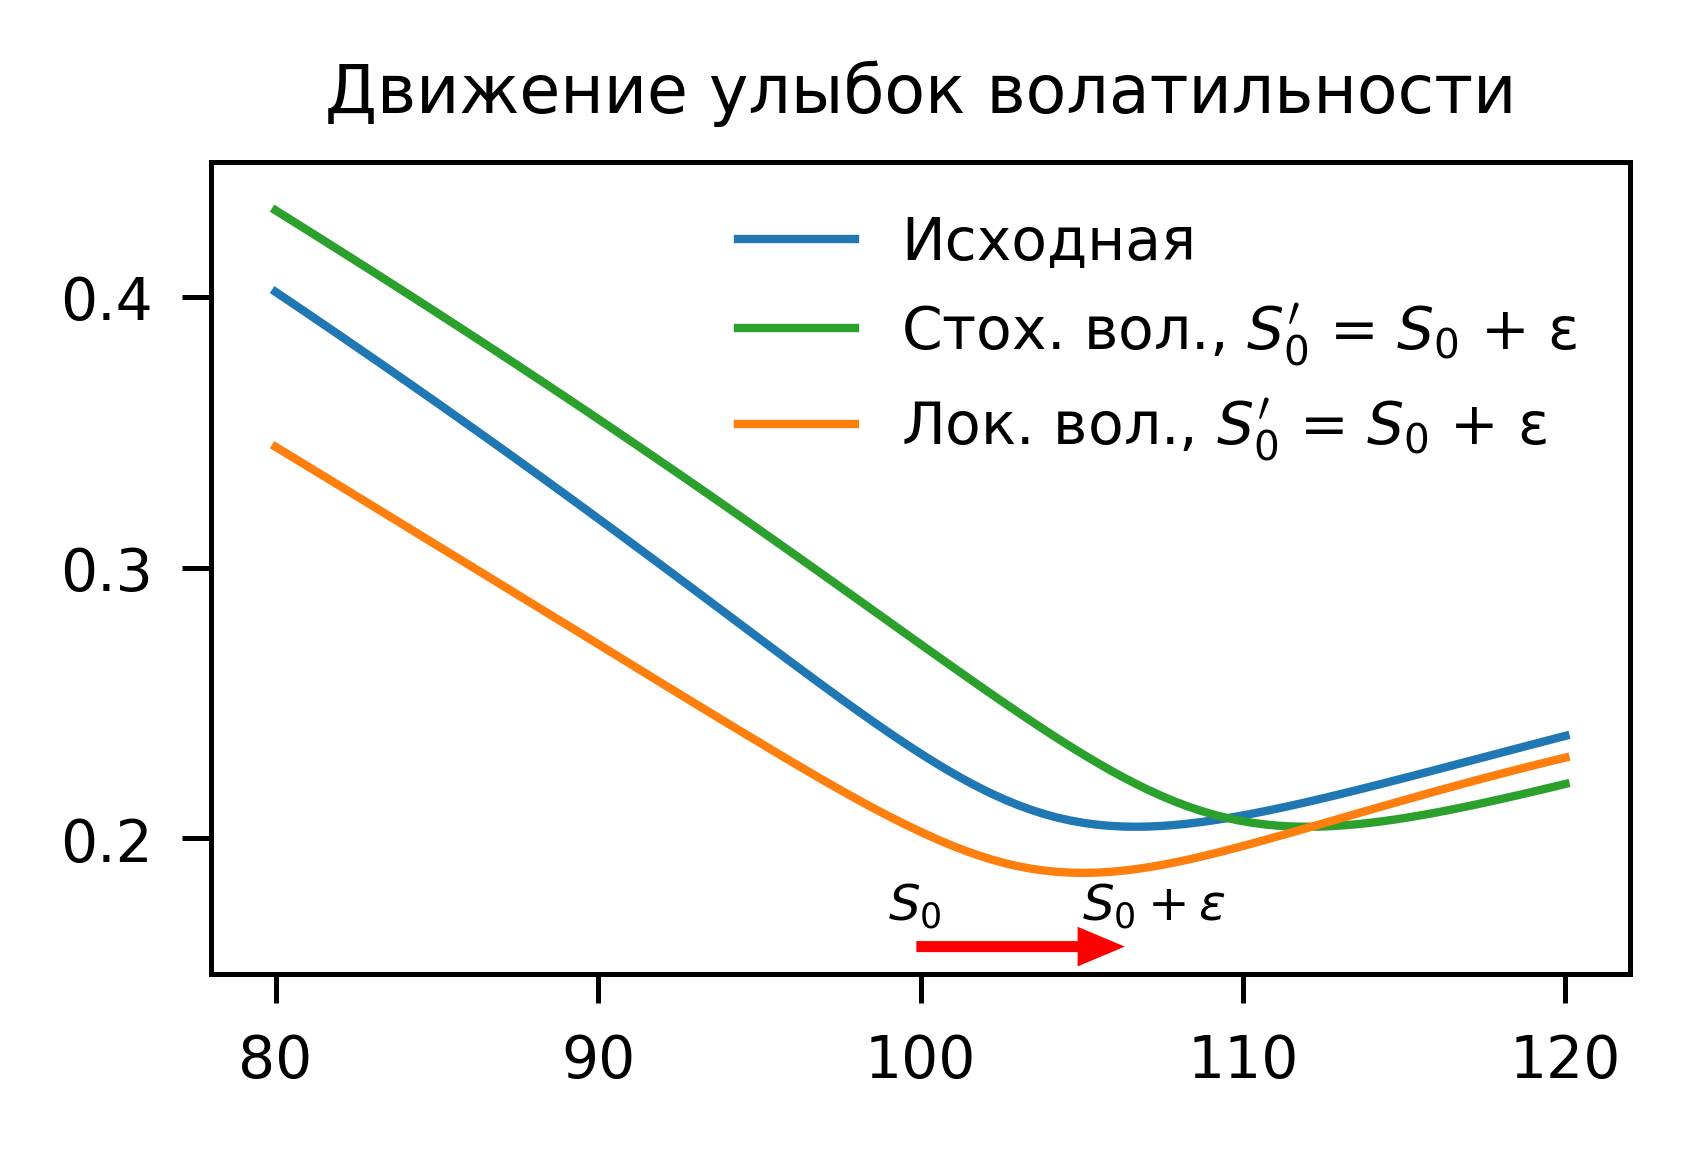
\includegraphics{pic/locvol-iv.png}
\centering
\caption{Изменение улыбок волатильности в модели локальной волатильности и модели стохастической волатильности при изменении цены базового актива.}
\label{lv:f:iv-move}
\end{figure}



\section{Вспомогательные результаты}
В этом разделе собраны технические результаты, которые потребуются для доказательства формулы Дюпира.
Приводимое доказательство следует книге \cite{MusielaRutkowski09}.
Оригинальное доказательство Б.~Дюпира приведено в разделе \ref{lv:s:dupire-proof}.

\subsection{Формула Бридена--Литценбергера}

Следующий результат в приложениях к оценке опционов впервые встречается в работе Д.~Бридена и Р.~Литценбергера \cite{BreedenLitzenberger78} и поэтому в литературе часто называется \emph{формулой Бридена"--~Литценбергера}.

\begin{proposition}
\label{1:l:bl}
Пусть $S\ge 0$ "--- случайная величина, $\E S<\infty$.
Обозначим $C(K) = \E(S-K)^+$, $K\in\R_+$.
Предположим, что $C\in C^2((0,\infty))$.
Тогда $S$ имеет абсолютно непрерывное распределение с плотностью $f(s)=C''(s)$.
\end{proposition}

\begin{proof}
Имеем $C(K) = \int_K^\infty (s-K) d F(s) = \int_K^\infty (K-s) d (1-F(s))$, где $F$ "--- функция распределения $S$.
Интегрируя по частям%
\footnote{Для интеграла Лебега"--~Стилтьеса справедлива следующая формула интегрирования по частям (см.~\cite{Shiryaev04}, гл.~II, \S\,6, теорема 11).
Пусть функции $F$, $G$ имеют ограниченную вариацию на отрезке $[a,b]$, причем $F$ непрерывна справа и имеет пределы слева в каждой точке, а $G$ непрерывна.
Тогда $F(b)G(b) - F(a)G(a) = \int_a^b F(x)d G(x) + \int_a^b G(x) d F(x)$.},
получаем
\[
C(K) = \lim_{b\to\infty} \left((K-b)(1-F(b)) + \int_K^b (1-F(s)) ds\right).
\]
Заметим, что $\lim\limits_{b\to\infty} b(1-F(b)) = 0$. Действительно, 
\[
0 = \lim\limits_{b\to\infty} \E S\I(S> b) \ge \lim_{b\to\infty} b \P(S> b) = \lim\limits_{b\to\infty} b(1-F(b)),
\]
где в первом равенстве воспользовались теоремой о мажорируемой сходимости и тем, что $\E S < \infty$.
Тогда $C(K) = \int_K^\infty (1-F(s)) ds$, откуда $C'(K) = F(K) - 1$.
Следовательно, $F(s)$ непрерывно дифференцируема и $f(s) = C''(s)$.
\end{proof}

\begin{remark}[смысл формулы Бридена"--~Литценбергера]
Пусть безрисковая процентная ставка равна 0.
Тогда, согласно формуле Бридена--Литценбергера, поверхность цен опционов колл $\hat C(T,K)$ задает семейство одномерных плотностей $f_t(s) = \hat C''_{KK}(t,s)$.
С другой стороны, цены опционов в модели $C(T,K) := \E(S_T-K)^+$ определяются одномерными распределениями величин $S_T$.
Таким образом, имеется взаимно-однозначное соответствие между ценами опционов колл (или пут) и одномерными распределениями процесса цены относительно эквивалентной мартингальной меры (при условии, что функция $C(T,K)$ и распределения величин $S_T$ достаточно хорошие). 
Рассуждение остается справедливым и в случае произвольной безрисковой ставки.

Как следствие, модель локальной волатильности можно рассматривать как модель, воспроизводящую заданные одномерные распределения процесса цены рискового актива. 
\end{remark}


\subsection{Локальное время}

Подробное изложение результатов о \emph{локальных временах} случайных процессов можно найти в книге \cite{RevuzYor}, гл.~VI; здесь же мы приведем без доказательств только нужные нам факты.

Далее в этом разделе $X$ "--- локальный мартингал вида%
\footnote{Все приводимые результаты остаются верными и для произвольных непрерывных локальных мартингалов, но в формулах нужно будет заменить $\sigma_t^2 dt$ на $d\qc X_t$, где $\qc X_t$ "--- \emph{квадратическая характеристика} непрерывного локального мартингала $X$, \te\  неубывающий непрерывный согласованный процесс такой, что $X_t^2 - \qc X_t$ является локальным мартингалом.}
$d X_t = \sigma_t d W_t$.

\begin{proposition}[\emph{формула Танаки}, \cite{RevuzYor}, гл.~VI, теоремы 1.2 и 1.7]
Для любого $a\in \R$ существует \as-единственный неубывающий непрерывный согласованный процесс $L_t^a(X)$ такой, что 
\[
|X_t - a| = |X_0-a| + \int_0^t \sgn(X_s-a) d X_s + L_t^a(X),
\]
где $\sgn(x) = 1$ для $x\ge 0$ и $\sgn(x)=-1$ для $x< 0$ (так, что правая производная $|x|' = \sgn(x))$.

Более того, существует модификация процесса $L_t^a(X)$, которая непрерывна по паре переменных $(t,a)$.
\end{proposition}

\begin{definition}
Процесс $L_t^a(X)$ называется \emph{локальным временем} процесса $X$ на уровне $a$.
\end{definition}

Далее всегда будем рассматривать модификацию локального времени, которая непрерывна по паре переменных.

\begin{remark}
Формула Танаки обобщает формулу Ито на негладкую функцию $f(x) = |x-a|$. 
По формуле Ито $|X_t - a| = |X_0-a| + \int_0^t \sgn(X_s-a) d X_s + \int_0^t f''(X_s) \sigma_s^2 ds$, однако производная $f''$ не определена.
Формула Танаки говорит, что вместо $\int_0^t f''(X_s) \sigma_s^2 ds$ нужно поставить локальное время.
\end{remark}


\medskip
Напомним, что если функция $f$ выпукла на $\R$, то у нее в каждой точке существует левая и правая производная; левая производная непрерывна слева, а правая справа, причем обе производные не убывают.
В частности, из этих свойств следует, что для выпуклой функции можно определить $\sigma$-конечную меру на $\R$ по формуле $\mu_f((a,b]) = f'(b) - f'(a)$, где $f'$ "--- правая производная.
Далее будем обозначать ее как $f''(da)$.

\begin{proposition}[\emph{формула Ито--Танаки--Мейера}, \cite{RevuzYor}, гл.~VI, теорема 1.5]
Если функция $f(x)$ выпукла, то 
\[
f(X_t) = f(X_0) + \int_0^t f'_-(X_s) dX_s + \frac12 \int_\R L_t^a(X) f''(da).
\]
\end{proposition}

\begin{example}
Если $f(x) = (x-a)^+$, то правая производная $f'(x) = \I(x\ge a)$. Тогда
\[
(X_t-a)^+ = (X_0-a)^+ + \int_0^t \I(X_t\ge a) dX_t + \frac12 L_t^a(X).
\]
\end{example}

\begin{proposition}
\label{lv:l:martingale}
Пусть локальный мартингал $X_t$ вида $dX_t = \sigma_t dW_t$ является настоящим мартингалом.
Тогда для любого $a\in\R$ процесс $Y_t = \int_0^t \I(X_t\ge) d X_t$ тоже является мартингалом. 
Как следствие, справедливо равенство
\[
\frac12\E L_t^a(X) = \E(X_t-a)^+ - (X_0-a)^+.
\] 
\end{proposition}

% \begin{proof}
% По неравенству Йенсена процесс $(X_t-a)^+$ является субмартингалом.
% Из \emph{разложения Дуба"--~Мейера}%
% \footnote{Любой субмартингал $S_t$ представим в виде $S_t = S_0 + M_t + A_t$, где $M_t$ "--- локальный мартингал, $A_t$ "--- процесс ограниченной вариации, $M_0=A_0=0$, причем процессы $M_t$ и $A_t$ единственны \as{}}
%  следует, что его можно представить в виде $(X_t-a)^+ = (X_t-a)^+ + M_t + A_t$, где $M_t$ "--- непрерывный локальный мартингал, $A_t$ "--- непрерывный неубывающий согласованный процесс, $M_0=A_0=0$. 
% По формуле Ито"--~Танаки"--~Мейера имеем $(X_t-a)^+ = (X_0-a)^+ + \int_0^t \I(X_t>a) d X_t + \frac12 L_t^a(X)$, и следовательно
% \[
% M_t - \int_0^t \I(X_t>a) d X_t = \frac12 L_t^a(X) - A_t.
% \]
% Левая часть является непрерывным локальным мартингалом, а правая "--- непрерывным процессом ограниченной вариации. Из единственности в разложении Дуба"--~Мейера следует, что они обе нулевые. Таким образом, $\int_0^t \I(X_t>a) d X_t = M_t$ "--- мартингал.
% \end{proof}

% \begin{proof}
% По формуле Ито"--~Танаки"--~Мейера имеем $(X_t-a)^+ = (X_0-a)^+ + \int_0^t \I(X_t>a) d X_t + \frac12 L_t^a(X)$.
% Вычисляя математическое ожидание от обеих частей и применяя лемму \ref{lv:l:martingale}, получаем доказываемое утверждение.
% \end{proof}

Короткое доказательство предложения \ref{lv:l:martingale} для более общего случая можно найти в статье \cite{HamzaKlebaner22}. 


\begin{proposition}[формула для времени пребывания, \cite{RevuzYor}, гл.~VI, теорема 1.6]
Для любой неотрицательной измеримой функции $f(x)$ выполнено равенство
\[
\int_\R f(a) L_t^a(X) da = \int_0^t f(X_s) \sigma_s^2 ds.
\]  
\end{proposition}

\begin{remark}
Поясним, откуда возникает формула для времени пребывания.
Можно дать эквивалентное определение локального времени:
\[
L_t^a(X) = \lim_{\epsilon\downarrow 0} \frac{1}{2\epsilon} \int_0^t \I(|X_s-a|< \epsilon) \sigma^2_s ds.
\]
По своему смыслу эта формула означает, что локальное время является плотностью \emph{меры времени пребывания в точке $a$} (см.~\cite{RevuzYor}, гл.~VI, следствие 1.9), где мера пребывания $\mu$ "--- это случайная мера 
\[
\mu_t(\omega, A) = \int_0^t \I(X_s \in A) ds,
\] 
для борелевских множеств $A$.
Если приближать измеримую функцию $f$ простыми функциями (линейными комбинациям индикаторов), то из этого определения и получается формула времени пребывания.
\end{remark}


\section{Доказательство формулы Дюпира}
\subsection{Случай нулевой процентной ставки}

Пусть сначала $r_t\equiv 0$.
Согласно предложению \ref{lv:l:martingale}, 
\[
C(T,K) = (S_0-K)^+ + \frac 12 \E L_T^K(S).
\]
Обозначим $f(t,s)$ плотность величины $S_t$.
Тогда, умножая обе части полученного равенства на произвольную гладкую функцию $h(s)$ с компактным носителем и интегрируя, получаем
\begin{multline*}
\int_\R h(K) C(T,K) dK 
= \int_\R h(K)(S_0-K)^+  dK + \frac12 \E \int_0^T h(S_t) \sigma^2(t,S_t) S_t^2 dt \\
=\int_\R h(K)(S_0-K)^+  dK + \frac12 \int_0^T \int_\R h(K)f(t,K) \sigma^2(t,K)K^2 dK dt \\
= \int_\R h(K) 
  \biggl(
    (S_0-K)^+ + \frac12\int_0^T C''_{KK}(t,K) \sigma^2(t,K)K^2 dt
  \biggr) dK,
\end{multline*}
где в первом равенстве воспользовались формулой времени пребывания, во втором представили математическое ожидание в виде интеграла по плотности и поменяли пределы интегрирования, а в третьем равенстве воспользовались формулой Бридена"--~Литценбергера.
В силу произвольности функции $h$ из совпадения интегралов получаем равенство подынтегральных функций
\[
C(T,K) = (S_0-K)^+ + \frac12 \int_0^T C''_{KK}(t,K) \sigma^2(t,K) K^2dt.
\]
Дифференцируя по $T$, получаем доказываемое утверждение.

\subsection{Общий случай}
\label{lv:ss:general-case}
Покажем как случай произвольной детерминированной процентной ставки $r_t$ можно свести к $r_t\equiv 0$.
Для заданной функции $C(T,K)$ и функции $\sigma(t,s)$, определяемой по формуле Дюпира \eqref{lv:dupire}, введем две новые функции
\[
\hat C^*(T,K) = \hat C(T,KB_T), \qquad 
\sigma^*(t,s) = \sigma(t, sB_t).
\]
Непосредственно проверяется, что
\[
\sigma^*(t,s) = \sqrt{\frac{2(\hat C^*)'_T(t,s)}{s^2(\hat C^*)''_{KK}(t,s)}}.
\]
Кроме того, используя формулу Ито, находим, что, если процесс $S_t$ удовлетворяет уравнению \eqref{lv:model} с функцией $\sigma(t,s)$, то дисконтированная цена $S_t^* = S_t/B_t$ удовлетворяет уравнению $d S_t^* = \sigma^*(t,S_t^*) S_t^* d W_t$.

Таким образом, к функциям $\hat C^*$, $\sigma^*$ и процессу $S_t^*$ можно применить доказываемую теорему в случае $r_t\equiv 0$, откуда следует, что цены опционов $C^*(T,K) = \E(S_T^*-K)^+$  удовлетворяют равенству $C^*(T,K)=\hat C^*(T,K)$. 

Остается заметить, что $C(T,KB_T) = B_T^{-1} \E(S_T-KB_T)^+ = \E(S_T^* - K)^+ = C^*(T,K)$, и, следовательно, $C(T,KB_T) = \hat C(T,KB_T)$.
Тогда $C(T,K) = \hat C(T,K)$.


\subsection{Другое доказательство}
\label{lv:s:dupire-proof}

Приводимая далее цепочка равенств следуют рассуждениям в статье \cite{Dupire94}.
Некоторые переходы в ней трудно обосновать строго, поэтому ее нельзя назвать формальным доказательством.

Рассмотрим только случай $r_t\equiv 0$.
Пусть $f(t,s)$ "--- плотность $S_t$.
Тогда
\[
\begin{split}
C'_T(T,K) 
&= \int_K^\infty (s-K) \prt ft(T,s) ds 
  = \text{[прямое уравнение Колмогорова]} \\[1em] 
&= \frac12 \int_K^\infty (s-K)\prtt{}{s}(\sigma^2 s^2 f)(T,s) ds 
  = \text{[интегрирование по частям]}\\[1em] 
&= -\frac12\int_K^\infty \prt{}s (\sigma^2y^2f)(T,s) ds \\[1em]
&= \frac12 \sigma^2(T,K)K^2 f(T,K)
  = \text{[формула Бридена--Литценбергера]}\\[1em]
&= \frac12 \sigma^2(T,K) K^2 C''_{KK}(T,K).
\end{split}
\]
Получаем, что если $C(T,K)$ "--- цены опционов колл в модели, то функция $\sigma(t,s)$ должна удовлетворять равенству $\sigma^2(t,s) = 2C'_T(t,s)/C''_{KK}(t,s)$.
Соответственное, если модель воспроизводит рыночные цены опционов ($C=\hat C$), то верна формула Дюпира \eqref{lv:dupire}.


\section{Алгоритм Андреасена"--~Хьюджа}
\label{lv:s:ah}
\subsection{Построение локальной волатильности по дискретным ценам опционов}
Пусть задан конечный набор времен исполнения $T_1<T_2<\ldots<T_m$ и для каждого времени исполнения задан набор цен опционов колл $\hat C_{i,j}=\hat C(T_i, \hat K_{i,j})$, где $\hat K_{i,1} < \ldots < \hat K_{i,n_i}$ "--- различные страйки.
В этом разделе мы приведем алгоритм Андреасена"--~Хьюджа \cite{AndreasenHuge10} построения функции локальной волатильности $\sigma(t,s)$ по ценам $\hat C_{i,j}$.

Далее будем считать безрисковую ставку равной 0.
В случае ненулевой ставки можно построить локальную волатильность $\sigma^*(t,s)$ для дисконтированного процесса цены (для этого нужно применить тот же самый алгоритм, но считая, что вместо страйков $\hat K_{i,j}$ заданы страйки $\hat K_{i,j} B_{T_i}$, а цены опционов те же "--- это следует из рассуждений в доказательстве формулы Дюпира, см.~раздел \ref{lv:ss:general-case}), и тогда искомая локальная волатильность будет $\sigma(t,s) = \sigma^*(t,s/B_t)$. 

Положим $T_0=0$.
Функция $\sigma(t,s)$ будет кусочно-постоянной по $t$ на промежутках $(T_{i-1}, T_i]$ и кусочно-линейной по $s$ на промежутках $(\hat K_{i,j-1}, \hat K_{i,j}]$, а именно для $t\in (T_{i-1}, T_i]$ положим
\[
\sigma(t, s) = \begin{cases}
a_{i,1}, 
  &\text{при } s\le \hat K_{i,1},\\
\dfrac{a_{i,j-1}(s-\hat K_{i,j-1}) + a_{i,j}(\hat K{i,j} - s)}{\hat K_{i,j}-\hat K_{i,j-1}}, 
  &\text{при } \hat K_{i,j-1}< s \le \hat K_{i,j},\\
a_{i,n_i}, 
  &\text{при } s> \hat K_{i,n_i},
\end{cases}
\]
где значения $a_{i,j}$ предстоит найти.
Идея состоит в том, что по значениям $a_{i,j}$ можно вычислить цены опционов $C(T, K)$ в модели, и, следовательно, нужно выбрать $a_{i,j}$ так, чтобы получаемые цены в точках $(T_i, K_{i_j})$ были как можно ближе к заданным значениям $\hat C_{i,j}$.

Покажем, как по выбранным $a_{i,j}$ найти цены опционов в модели.
Будем искать функцию $C(T,K)$ для $T=T_i$ по индукции. Для $i=0$ положим $C(0, K) = (S_0-K)^+$.
Далее воспользуемся тем, что формулу Дюпира можно записать в виде
\[
C'_T(T,K) = \frac12 K^2 \sigma^2(T,K)C''_{KK}(T,K).
\]
Если функция $C(T_{i-1}, K)$ построена, то, дискретизируя производную по $T$, получаем дифференциальное уравнение на функцию $C(T_i,K)$:
\[
\frac{C(T_{i},K) - C(T_{i-1},K)}{\Delta T_i} = \frac12 K^2 \sigma^2(T_i,K)C''_{KK}(T_i,K),
\]
где $\Delta T_i = T_i - T_{i-1}$.
Чтобы его решить, воспользуемся методом конечных разностей и дискретизируем производную по $K$.
Для этого зафиксируем набор страйков $K_0,\dots,K_m$, где $K_l = K_0 + l\Delta K$, так что $K_0$ достаточно мало, а $K_m$ достаточно велико.
Будем использовать один и тот же набор $K_l$ для всех значений $T_i$, поэтому промежуток $(K_0, K_m)$ должен, как минимум, покрывать все страйки $\hat K_{i,j}$, для которых нам даны цены $\hat C_{i,j}$.

Для $l=1,\dots,m-1$ получаем разностные уравнения
\begin{multline}
\label{lv:ah-system}
\frac{C(T_i,K_l) - C(T_{i-1}, K_l)}{\Delta T_i} \\
= \frac12 K_l^2 \sigma^2(T_i,K_l) \frac{C(T_i,K_{l-1}) -2C(T_i,K_l) + C(T_i,K_{l+1})}{(\Delta K)^2}.
\end{multline}
Для $l=0$ и $l=m$ добавим условия $C''_{KK}(T_i,K_l) = 0$, что даст уравнения
\begin{gather}
\label{lv:ah-boundary-1}
C(T_i,K_0) - C(T_{i-1}, K_0) = 0,\\
\label{lv:ah-boundary-2}
C(T_i,K_m) - C(T_{i-1}, K_m) = 0.
\end{gather}

Систему линейных уравнений \eqref{lv:ah-system}--\eqref{lv:ah-boundary-2} можно представить в матричном виде $A c_i = c_{i-1}$, где $c_i=(c_{i,0},\dots,c_{i,l})$ "--- вектор неизвестных, соответствующих значениям $C(T_i,K_l)$, а матрица $A$ имеет трехдиагональный вид
\[
A = \begin{pmatrix}
1 & 0 \\
-z_1 &1+2z_1 & -z_1\\
& -z_2 &1+2z_2 & -z_2\\
& & \ddots & \ddots & \ddots \\
& & & -z_{m-1} &1+2z_{m-1} & -z_{m-1}\\
& & & & 0 & 1
\end{pmatrix},
\]
где
\[
z_l = \frac{\Delta T_i}{2(\Delta K)^2} K_l^2\sigma^2(T_i,K_l).
\]
Матрица $A$ обладает свойством строгого диагонального преобладания (каждый элемент на главной диагонали по модулю больше суммы модулей других элементов в строке), и хорошо известно, что такие матрицы обратимы.
Следовательно, рассматриваемая система уравнений имеет единственное решение.
Трехдиагональный вид позволяет эффективно находить его численно, например, \emph{методом прогонки}.

Пусть $c_i(a_i)$ обозначает решение этой системы, зависящее от вектора параметров $a_i=(a_{i,1},\dots,a_{i,n_i})$. 
Тогда для выбора $a_i$ решается оптимизационная задача
\[
\sum_{j=1}^{n_i} (\hat C_{i,j} - c_{i,j}(a_i))^2 \to \text{min}.
\]
После нахождения $a_i$ переходят к аналогичной процедуре для нахождения $a_{i+1}$, и так далее.


\subsection{Интерполяция цен опционов}
Алгоритм Андреасена"--~Хьюджа также используется для интерполяции цен опционов, \te\ нахождения $\hat C(T,K)$ в точках, отличных от $(T_i,K_{i,j})$.

Пусть $T\in(T_{i-1},T_i)$ (или $T>T_m$ "--- для задачи экстраполяции).
Тогда значения $C(T,K_l)$ находятся из решения системы \eqref{lv:ah-system}--\eqref{lv:ah-boundary-2} с $T$ вместо $T_i$, \te\ решая $Ac = c_{i-1}$, где $c$ "--- вектор неизвестны цен $C(T,K_l)$, а матрица $A$ имеет такой же вид, как и выше, но с элементами
\[
z_l = \frac{T-T_{i-1}}{2(\Delta K)^2} K_l^2\sigma^2(T_i,K_l).
\]
После нахождения $C(T,K_l)$ цены в промежуточных точках $K\in (K_0,K_m)$ можно получить линейной интерполяцией, а для $K< K_0$ или $K>K_m$ экстраполировать цены в виде $C(T,K) = (S_0-K)^+$ (это соответствует тому, что выше мы считали $C''_{KK}(T_i,K_0) = C''_{KK}(T_i,K_m) = 0$, что вместе с начальным условием $C(0,K) = (S_0-K)^+$  по формуле Дюпира дает равенство $C(T_i,K_l) = C(T_i,K_l) = (S_0-K_l)^+$ для $l=0,m$.)


\summary
\begin{itemize}
\item Модель локальной волатильности: $d S_t = r_tS_t dt + \sigma(t,S_t)S_t d W_t$, где функцию $\sigma(t,s)$ нужно выбрать так, что модель будет в точности воспроизводить рыночные цены опционов колл (и, следовательно, цены опционов пут).

\item Формула Дюпира дает явное выражение для функции $\sigma(t,s)$ через поверхность рыночных цен опционов колл $\hat C(T,K)$:
\[
\sigma(t,s) = \sqrt{\frac{2(\hat C'_T(t,s) + r_ts\hat C'_K(t,s))}{s^2\hat C''_{KK}(t,s)}}.
\]

\item Достоинство модели локальной волатильности: точное воспроизведение цен опционов и подразумеваемых волатильности.
Недостаток: неверная динамика цен опционов и подразумеваемой волатильности.

\item Алгоритм Андреасена"--~Хьюджа позволяет построить локальную волатильность по дискретному набору цен опционов, а также интерполировать и экстраполировать цены опционов на значения времени исполнения и страйка, отсутствующие в рыночных данных.
\end{itemize}

%!TEX root=finmath2.tex

\chapter{Модель Хестона: цены европейских опционов}
\label{ch:heston-formula}
\chaptertoc

Модель Хестона (S.~Heston, 1993) "--- это одна из популярных моделей стохастической волатильности.
Ее главное достоинство состоит в том, что в ней имеется формула для цен европейских опционов колл и пут, которая сводится к вычислению некоторого интеграла, что позволяет быстро находить цены опционов численно.

\section{Описание модели}
\subsection{Уравнения, задающие модель}

Далее всегда будем считать, что исходная вероятностная мера $\P$ уже является мартингальной.
Кроме того, для простоты изложений и краткости формул мы будем предполагать, что безрисковая процентная ставка нулевая, а рисковый акив не платит дивиденды (о том, как к такому случаю свести общую модель, см.~раздел \ref{gen:s:forward} лекции \ref{ch:general}).

Цена рискового актива в модели Хестона описывается уравнениями
\begin{align}
\label{hes:S}
&dS_t = \sqrt{V_t}S_t d W_t^{(1)},\\
\label{hes:V}
&d V_t = \kappa(\theta-V_t)dt + \sigma\sqrt{V_t} d W_t^{(2)},
\end{align}
где процесс $V_t$ называется \emph{стохастической дисперсией} ($\sqrt{V_t}$ "--- \emph{стохастическая волатильность}), $W_t^{(1)},W_t^{(2)}$ "--- стандартные броуновские движения с коэффициентом корреляции $\rho\in(-1,1)$, \te\ $\E(W_t^{(1)}W_t^{(2)}) = \rho t$.
Величины $\kappa,\theta,\sigma>0$, $\rho\in(-1,1)$, а также начальное значение $V_0\ge 0$ являются параметрами модели, которые нужно оценить из рыночных данных.
Отметим, что процесс стохастической дисперсии $V_t$ "--- это процесс CIR, рассмотренный в лекции \ref{ch:sde}.

Начальные значения $S_0$ и $V_0$ далее всегда будет считаться строго положительными.

\begin{proposition}
Система уравнений \eqref{hes:S}--\eqref{hes:V} имеет единственное сильное решение $(S,V)$, причем процесс $S_t$ строго положителен.
Двумерный процесс $(S_t,V_t)$ является строго марковским.
Если $2\kappa\theta\ge \sigma^2$, то процесс $V_t$ строго положителен. 
\end{proposition}

\begin{proof}
Существование единственного сильного решения уравнения \eqref{hes:V}, а также то, что условие $2\kappa\theta\ge\sigma^2$ (условие Феллера) приводит к положительности решения, обсуждалось в лекции \ref{ch:sde}.
Сильное решение уравнения \eqref{hes:S} можно построить в явном виде:
\[
S_t = S_0 e^{\int_0^t \sqrt{V_s} dW_s^{(1)}  - \frac12 \int_0^t V_s ds}.
\]
Проверка того, что это действительно решение, проводится по формуле Ито.
Единственность (впрочем, как и существование) вытекает из того, что $S_t$ является \emph{стохастической экспонентой} процесса $d X_t = \sqrt{V_t} dW_t^{(1)}$ и общего результата о существовании и единственности стохастической экспоненты (см.~подробнее приложение \ref{ch:stoch-exp}).

Строго марковское свойство процесса $(S,V)$ следует из существования и единственности решения (см.~теорему \ref{sde:t:strong-markov} в лекции \ref{ch:sde}).
\end{proof}

Можно дать следующую интерпретацию параметрам процесса стохастической дисперсии.
Во-первых, заметим, что
\begin{equation}
\label{hes:EV}  
\E V_t = \theta + (V_0 - \theta)e^{-\kappa t}.
\end{equation}
Эта формула получается, если взять математическое ожидание от обеих частей интегральной формы уравнения \eqref{hes:V}.
Тогда, обозначая, $f(t) = \E V_t$, получаем уравнение $f(t) = V_0 + \kappa\int_0^t (\theta - f(s))ds$, решением которого является \eqref{hes:EV}.

Таким образом, процесс $V_t$ обладает свойством возврата к уровню $\theta$, называемому \emph{долгосрочным средним}.
Параметр $\kappa$ задает \emph{скорость возврата} к $\theta$.
Параметр $\sigma$ называют \emph{волатильностью волатильности} (\emph{vol-of-vol}), он контролирует насколько сильны колебания волатильности.


\subsection{Мартингальность процесса цены \difficult}

Напомним (см.~лекцию \ref{ch:general}), что желательным свойством любой модели является настоящая (не локальная) мартингальность цены рискового актива $S_t$.

\begin{proposition}
\label{hes:p:price-martingale}
В модели Хестона процесс $S_t$ является мартингалом.
\end{proposition}

Доказательство будет состоять в проверке условия Новикова.
Для этого мы ограничим процесс $V_t$ сверху подходящим процессом $V_t'$, для которого условие Новикова легко проверяется.
Потребуется следующий вспомогательный результат, который можно найти в \cite{KaratzasShreve91}, гл.~5, предложение 2.18.

\begin{lemma}[\emph{теорема сравнения} для стохастических дифференциальных уравнений]
Пусть $X^{(1)}$ и $X^{(2)}$ "--- сильные решения уравнений
\[
d X_t^{(i)} = a^{(i)}(t, X_t^{(i)}) dt + b(t,X_t^{(i)}) d W_t, \qquad X_0^{(i)} = x_0^{(i)},
\]
заданные на одном вероятностном пространстве.
Предположим, что выполнены следующие условия:
\begin{enumerate}
\item функции $a^{(i)}(t,x)$, $b(t,x)$ непрерывны;
\item $|a^{(i)}(t,x) - a^{(i)}(t,y)| \le K|x-y|$ с некоторой константой $K>0$ для всех $t,x$ и хотя бы одного $i=1,2$;
\item найдется возрастающая функция $h(x)$ такая, что $h(0) = 0$, $\int_0^\epsilon h(x) dx = \infty$ для любого $\epsilon>0$, а также $|b(t,x) - b(t,y)| \le h(|x-y|)$ для всех $x,y$;
\item $x_0^{(1)} \le x_0^{(2)}$;
\item $b^{(1)}(t,x) \le b^{(2)}(t,x)$ для всех $t,x$;
\end{enumerate}
Тогда $X_t^{(1)} \le X_t^{(2)}$ \as\ для всех $t\ge 0$.
\end{lemma}

\begin{proof}[Доказательство предложения~\ref{hes:p:price-martingale}]
Как было отмечено выше, процесс $S_t$ является стохастической экспонентой процесса $d X_t = \sqrt{V_t}dW_t^{(1)}$.
Следовательно, для того, чтобы $S_t$ был мартингалом, достаточно выполнения условия Новикова (см.~приложение~\ref{ch:stoch-exp})
\[
\E \exp\biggl(\frac12 \int_0^T V_t dt\biggr) < \infty.
\]
В свою очередь, для этого достаточно (см.~следствие \ref{stochexp:novikov-corollary} в приложении \ref{ch:stoch-exp}), чтобы для некоторого $\epsilon>0$ и для всех $t\in[0, T-\epsilon]$ было выполнено неравенство
\[
\E \exp\biggl(\frac12 \int_t^{t+\epsilon} V_s ds\biggr) < \infty.
\]
Заметим, что по неравенству Йенсена $\exp(\int_t^{t+\epsilon} \frac 12 V_s ds) \le \frac1\epsilon\int_t^{t+\epsilon} \exp(\frac\epsilon2 V_s) ds$, а поэтому
\begin{equation}
\label{hes:mart-bound}
\E \exp\biggl(\frac12 \int_t^{t+\epsilon} V_s ds\biggr) 
\le \frac1\epsilon \int_t^{t+\epsilon} \E e^{\frac\epsilon2 V_s} ds.
\end{equation}
Оценим $\E e^{\frac\epsilon2 V_s}$.
Положим $n = 4\lceil \kappa\theta/\sigma^2 \rceil$, $ \alpha = \kappa/2$ и рассмотрим процесс
\[
d V_t' = (n\sigma^2/4 - 2\alpha V'_t) dt + \sigma\sqrt{V_t'} d W_t^2, \qquad V_0' = V_0.
\]
Параметры $n$ и $\alpha$ выбраны так, что для всех $v\ge0$ выполнено неравенство $n\sigma^2/4-2\alpha v \ge \kappa (\theta-v)$.
Тогда, используя теорему сравнения, находим, что 
\[
V_t' \ge V_t\ \text{\as\ для всех $t\ge 0$}.
\]

Таким образом, достаточно будет оценить сверху подходящим образом ожидание $\E e^{\frac\epsilon2 V_t'}$.
Для этого покажем, что верно равенство по распределению $V_t' \stackrel{d}{=} U_t$ для процесса
\[
U_t = \sum_{i=1}^n (Y_t^{(i)})^2,
\]
где $Y^{(i)}$ "--- независимые процессы Орнштейна"--~Уленбека
\[
d Y_t^{(i)} = -\alpha Y_t^{(i)} dt +  \frac\sigma2 d B_t^{(i)}
\]
с начальными условиями $Y_0^{(i)}$ такими, что $\sum_i (Y_0^{(i)})^2 = V_0'$.

Действительно, применяя формулу Ито, получаем
\[
d U_t = \left(\frac{n\sigma^2}{4}-2\alpha U_t\right) dt + \sum_{i=1}^n Y_t^{(i)} d B_t^{(i)} = 
\left(\frac{n\sigma^2}{4}-2\alpha U_t\right) dt + \sigma \sqrt{U_t} d Z_t
\]
с процессом 
\[
d Z_t = \frac{\sum_i Y_t^{(i)}}{\sigma \sqrt{U_t}} d B_t^i.
\]
Процесс $Z_t$ является локальным мартингалом.
Кроме того, его квадратическая характеристика равна $t$ (\te\ $Z_t^t -t $ является локальным мартингалом), в чем нетрудно убедиться по формуле Ито, показав, что дифференциал $d(Z_t^2 - t)$ не содержит члена с $dt$.
Отсюда по теореме Леви%
\footnote{Непрерывный локальный мартингал с нулевым начальным значением является стандартным броуновским движением тогда и только тогда, когда его квадратическая характеристика равна $t$.}
следует, что $Z_t$ "--- стандартное броуновское движение и, значит, $U_t$ удовлетворяет тому же уравнению, что и $V_t'$, \te\ является процессом CIR с теми же параметрами.
Таким образом, $U$ и  $V'$  совпадают по распределению.

Так как процессы Орнштейна"--~Уленбека $Y_t^i$ имеют гауссовские распределения, то для любого $c>1$ и всех $t\in[0,T]$ найдется малое $\epsilon>0$ такое, что $\E e^{\frac\epsilon2 (Y_t^i)^2} < c$, и тогда
\[
\E e^{\frac\epsilon2 V_t'} \le c^n.
\]
Отсюда следует, что правая часть \eqref{hes:mart-bound} конечна, что нам и требовалось.
\end{proof}


\subsection{Условие для безарбитражности модели \difficult}

Выше мы предполагали, что исходная вероятностная мера $\P$ уже является мартингальной.
Если же относительно меры $\P$ процесс цены $S_t$ имеет произвольный коэффициент сноса, то вопрос о существовании эквивалентной мартингальной меры и выполнении свойства безарбитражности (NFLVR) становится деликатным и зависит от выполнения условия Феллера.
Для простоты изложения, ограничимся случаем постоянной безрисковой ставки $r$ и постоянного коэффициента сноса $\mu$.

\begin{proposition}[см.~\cite{DesmettreLeobacherRogers21}]
Пусть относительно меры $\P$ цена рискового актива задается уравнениями
\begin{align*}
&d S_t = \mu S_t dt + \sqrt{V_t} d W_t^{(1)},\\
&d V_t = \kappa(\theta-V_t)dt + \sigma \sqrt{V_t} d W_t^{(2)},
\end{align*}
где $\mu\neq r$ и $V_0,S_0>0$.
Тогда ЭЛММ в такой модели существует в том и только том случае, когда выполнено условие Феллера $2\kappa\theta\ge \sigma^2$.
\end{proposition}


\section{Формула для цены европейских опционов}

В этом разделе будет получена формула для цен ванильных опционов колл и пут в модели Хестона, которая сводится к вычислению некоторого интеграла.
Значение этого интеграла можно найти методами численного интегрирования.

Идея будет состоять в том, чтобы сначала выразить цену опциона через вероятности его исполнения относительно двух вероятностных мер, затем получить аналитическую формулу для характеристических функций логарифма цены рискового актива относительно этих мер и, обратив их, найти вероятности исполнения опциона.
Упомянутый выше интеграл будет возникать при обращении характеристических функций.

Далее будем рассматривать только опционы колл.
Цены опционов пут можно найти аналогично или воспользоваться паритетом цен колл-пут.


\subsection{Формулировка теоремы}

Зафиксируем время исполнения $T$. Определим функции
\begin{align*}
&\phi(u;t,x,v) = \exp(C(T-t,u) + D(T-t,u)v + iu x),& &u\in\R_+ \cup (\R_+-i),\\
&\tilde \phi(u;t,x,v) = e^{-x}\phi(u-i;t,x,v),& &u\in\R_+,
\end{align*}
где
\begin{align}
\label{hes:C}
&C(\tau,u) = \frac{\kappa\theta}{\sigma^2}
  \biggl(
    (\kappa- \rho\sigma iu - d(u))\tau 
    - 2\ln\biggl(\frac{1-g(u)e^{-d(u)\tau}}{1-g(u)}\biggr)
  \biggr),\\
\label{hes:D}
&D(\tau,u) = \frac{\kappa - \rho\sigma i u - d(u)}{\sigma^2}
  \biggl(\frac{1-e^{-d(u)\tau}}{1-g(u)e^{-d(u)\tau}}\biggr),\\
\label{hes:dg}
&d(u)=\sqrt{(\rho\sigma iu - \kappa)^2 + \sigma^2(iu + u^2)},\quad
  g(u) = \frac{\rho\sigma iu- \kappa +d(u)}{\rho\sigma iu - \kappa -d(u)}.
\end{align}
Здесь везде $i=\sqrt{-1}$ "--- мнимая единица. Множество $\R_+-i$ обозначает полупрямую в комплексной плоскости, параллельную неотрицательной действительной полуоси и исходящую из точки $-i$.
Переменные $t,x,v$ вещественные.

Как будет видно далее, $\phi$ является условной характеристической функцией $\E (e^{iu X_T}\mid X_t=x, V_t=v)$, где $X_t=\ln S_t$, а $\tilde \phi$ "--- это та же характеристическая функция, но вычисленная по другой мере.

В следующей теореме, как и прежде, считается, что безрисковая процентная ставка равна нулю, а базовый актив не выплачивает дивиденды.

\begin{theorem}[С.~Хестон]
\label{hes:t:formula}
Цена опциона колл со страйком $K$ и временем исполнения $T$ в момент времени $t$ равна
\begin{equation}
\label{hes:call-repr}
C_t = C(t,\ln S_t,V_t),
\end{equation}
где функция $C$ имеет вид
\begin{equation}
\label{hes:call-undiscounted}
C(t,x,v) = e^x \tilde \Pi(t,x,v) - K \Pi(t,x,v)
\end{equation}
с функциями $\tilde\Pi$, $\Pi$ определенными по формулам
\begin{align}
\label{hes:pi}
&\Pi(t,x,v) = \frac12 + \frac1\pi \int_0^\infty
  \mathrm{Re}\biggl(\frac{e^{-iu \ln K}\phi(t,x,v;u)}{iu}\biggr) du,\\[0.5em]
\label{hes:pit}
&\tilde\Pi(t,x,v) = \frac12 + \frac1\pi \int_0^\infty
  \mathrm{Re}\biggl(\frac{e^{-iu \ln K}\tilde \phi(t,x,v;u)}{iu}\biggr) du.
\end{align}
\end{theorem}

\begin{remark}
В формулах \eqref{hes:C} и \eqref{hes:dg} присутствуют комплексный корень и комплексный логарифм, являющиеся, вообще говоря, многозначными функциями.
Несмотря на то, что утверждение теоремы справедливо при любом выборе ветвей этих функций, удобнее всего здесь взять их главные значения%
\footnote{Напомним, что для числа $z\in\mathbb{C}$, записанного в виде $z=re^{i\phi}$, $r\ge 0$, $\phi\in(-\pi,\pi]$, главные значения логарифма и квадратного корня определены как $\ln z = \ln r + i\phi$ и $\sqrt{z} = \sqrt{r}e^{i\phi/2}$ (логарифм не определен для $z=0$).}. Это обеспечит непрерывность функций $C$ и $D$ на множестве $u\in\R_+$ и $u\in (\R_+-i)$, что хорошо сказывается на работе методов численного интегрирования для нахождения $\Pi$ и $\tilde\Pi$.

Доказательство непрерывности технически нетрудное, но достаточно громоздкое, см.~детали в статье \cite{Albrecher+07}.
Основная его идея состоит в том, что когда $u$ пробегает множество $\R_+$ или $\R_+-i$, аргументы логарифма и корня не пересекают отрицательную действительную полуось, что влечет их непрерывность в силу использования главных ветвей.
\end{remark}


\subsection{Доказательство}
\subsubsection{Представление цены опциона через вероятности исполнения}

Первый шаг будет состоять в том, чтобы выразить цену опциона колл через вероятности его исполнения по двум мерам.
Отметим, что приводимая ниже лемма выполнена не только в модели Хестона, но вообще в любой безарбитражной модели, при условии что безрисковая ставка равна 0, рисковый актив не выплачивает дивиденды, а его цена является настоящим мартингалом относительно меры $\P$.

Зафиксируем момент исполнения $T$ и определим новую вероятностную меру $\tilde\P$ с плотностью
\[
\frac{d\tilde\P}{d\P} = \frac{S_T}{S_0}. 
\]

\begin{lemma}
\label{hes:l:price-through-prob}
Цена опциона колл со страйком $K$ и временем исполнения $T$ в момент $t$ представима в виде 
\[
C_t = S_t \tilde\P(S_T\ge K\mid \F_t) - K\P(S_T\ge K\mid \F_t).
\]
\end{lemma}

\begin{proof}
Заметим, что
\[
C_t = \E^\P((S_T - K)^+\mid \F_t) = \E^\P(S_T \I(S_T\ge K) \mid \F_t) - K\P(S_T\ge K\mid \F_t).
\]
Пусть $Z = S_T/S_0$ обозначает плотность $d\tilde\P/d\P$. 
Тогда из формулы пересчета для условных математических ожиданий (см.~замечание ниже) находим
\begin{multline*}
\tilde\P(S_T\ge K\mid \F_t) = \E^{\tilde\P} (\I(S_T \ge K) \mid \F_t)
= \frac{\E^{\P}(Z \I(S_T \ge K)\mid \F_t)}{\E^{\P}(Z\mid \F_t)} \\= S_t \E^{\P}(S_T \I(S_T\ge K)\mid \F_t),
\end{multline*}
где воспользовались тем, что $\E(Z\mid \F_t) = S_t/S_0$, так как $S_t$ "--- мартингал относительно меры $\P$.
Подставляя получившееся равенство в формулу выше, получаем доказываемое утверждение.
\end{proof}

\begin{remark}
\emph{Формула пересчета} для условных математических ожиданий утверждает, что для двух мер $\tilde\P \sim \P$ с плотностью $Z=d\tilde\P/d\P$, произвольной $\sigma$-алгебры $\G\subseteq\F$ и $\tilde\P$-интегрируемой случайной величины $\sigma$ верно равенство (см.~\cite{Shiryaev04}, гл.~II, \S\,7, теорема 6)
\[
\E^{\tilde \P}(\xi\mid \G) = \frac{\E^{\P}(Z\xi\mid \G)}{\E^\P(Z\mid \G)}.
\]
\end{remark}


\subsubsection{Характеристчиеские функции логарифма цены}

Будем работать с процессом логарифма цены рискового актива
\[
X_t = \ln S_t.
\]
Для $t\le T$ определим условные характеристические функции
\begin{align*}
&\phi(u; t,x,v) = \E^{\P} (e^{iu X_T} \mid X_t=x, V_t = v), \qquad u\in\R_+ \cup (\R_+-i),\\
&\tilde\phi(u; t,x,v) = \E^{\tilde\P} (e^{iu X_T} \mid X_t=x, V_t = v), \qquad u\in\R_+ .
\end{align*}
Второй шаг в доказательстве теоремы \ref{hes:t:formula} "--- вычисление функций $\phi$ и $\tilde\phi$.
Для начала покажем, что вычисление $\tilde\phi$ можно свести к $\phi$.

\begin{lemma}
Справедливо равенство $\tilde \phi(u; t,x,v) = e^{-x}\phi(u-i;t,v,x)$.
\end{lemma}

\begin{proof}
Имеем
\[
\begin{split}
\tilde\phi(u; t,x,v) &= \E^{\tilde\P} (e^{iu X_T}  \mid X_t=x, V_t = v)
= \frac{\E^{\P} (Z e^{iu X_T} \mid X_t=x, V_t = v)}{\E^\P(Z \mid X_t=x,V_t=v)} \\
&= e^{-x} \E^{\P} (e^{i(u-i)X_T} \mid X_t=x, V_t = v)
= e^{-x}\phi(u-i; t,x,v),
\end{split}
\]
где воспользовались формулой пересчета для условных ожиданий, а также тем, что $Z=S_T/S_0$ и $\E^\P(S_T  \mid X_t=x, V_t = v) = e^x$, так как $S_t$ "--- мартингал.
\end{proof}

\begin{lemma}
Для любого $u\in \R$ функция $\phi(u;t,x,v)$ является единственным решением задачи Коши (в классе $C^{1,2}$ на $[0,T)\times\R\times\R_+$)
\begin{align}
\label{hes:cf-pde}
&\frac{\partial\phi}{\partial t} + \frac v2 \frac{\partial^2 \phi}{\partial x^2}  +\frac{\sigma^2v}{2} \frac{\partial^2\phi}{\partial v^2}
  + \rho\sigma v \frac{\partial^2\phi}{\partial x\partial v} -\frac v2 \frac{\partial \phi}{\partial x} 
  + \kappa(\theta-  v)\frac{\partial\phi}{\partial v} = 0,\\
\label{hes:cf-boundary}
&\phi(u;T,x,v) = e^{iu x}.
\end{align}
\end{lemma}

\begin{proof}
Этот результат напрямую следует из формулы \fc\ (см.~лекцию \ref{ch:sde}), примененной ее к вещественной и мнимой частям $\phi$.
\end{proof}

Покажем теперь, как решить задачу Коши \eqref{hes:cf-pde}--\eqref{hes:cf-boundary}.
Идея состоит в том, чтобы искать решение в специальном виде
\begin{equation}
\label{hes:cf}
\phi(u; t,x,v) = \exp(C(T-t,u) + D(T-t,u)v + iu x)
\end{equation}
с неизвестными функциями $C(\tau,u)$ и $D(\tau,u)$.
Чтобы их найти, подставим $\phi$ такого вида в \eqref{hes:cf-pde} и получим уравнение
\begin{equation}
\label{hes:CD-equation}
v\biggl(
  -\prt{D}\tau + \rho\sigma iu D - \frac12 u^2 
  + \frac12 \sigma^2 D^2 -\frac12 iu-\kappa D
\biggr) + \biggl(-\prt{C}\tau + \kappa\theta D\biggr) = 0.
\end{equation}
Равенство будет выполнено, если каждая из скобок тождественно равна нулю.
Заметим, что первая скобка не содержит функцию $C$, что приводит к обыкновенному дифференциальному уравнению на функцию $D$:
\[
D' = \rho\sigma ui D + \frac12 (\sigma^2 D^2 - iu - u^2) - \kappa D, \qquad D(0,u)=0,
\]
где штрих обозначает производную по переменной $\tau$, а переменная $u$ является фиксированным параметром.
Начальное условие $D(0,u)=0$ возникает из того, что $\phi(u,T,x,v) = \exp(iux)$ по определению функции $\phi$, а тогда из формулы \eqref{hes:cf} видно, что значение $D(0,u)$ должно быть равно 0 для всех $u$.

Уравнение для $D$ является \emph{дифференциальным уравнением Риккати} и решается известными методами.
Для удобства запишем его в виде
\[
D'= \alpha + \beta D + \gamma D^2,
\]
где
\[
\alpha = -\frac{iu + u^2}{2},\qquad \beta = \rho\sigma iu - \kappa, \qquad
\gamma = \frac{\sigma^2}{2}.
\]
Нетрудно проверить, что если функция $z(\tau)$ является решением уравнения
\[
z''(\tau) - \beta z(\tau) + \alpha\gamma z(\tau)= 0,
\]
то
\[
D(\tau,u) = -\frac{z'(\tau)}{\gamma z(\tau)} 
\]
является решением исходного уравнения.

Уравнение для $z(\tau)$ линейное, хорошо известно его общее решение.
Для этого рассмотрим характеристическое уравнение $r^2-\beta r+\alpha\gamma = 0$.
Непосредственно проверяется, что при любых значениях параметров модели Хестона и $u\in\R_+$ или $u\in(\R_+-i)$ дискриминант $d = \sqrt{(\rho\sigma iu - \kappa)^2 + \sigma^2(iu + u^2)}$ не обращается в нуль и, следовательно, общее решение имеет вид
\[
z(\tau) = K_1 e^{r_1\tau} + K_2 e^{r_2\tau},
\]
где $K_1,K_2$ "--- свободные константы, а $r_1=(\beta+d)/2$, $r_2=(\beta-d)/2$ "--- корни характеристического уравнения.
Это дает
\[
D(\tau) = -\frac1\gamma \biggl(\frac{K_1 r_1 e^{r_1\tau} + K_2 r_2e^{r_2\tau}}{K_1 e^{r_1\tau} + K_2e^{r_2\tau}} \biggr).
\]
Чтобы получить решение, удовлетворяющее начальному условию $D(0,u)=0$, выберем
\[
K_1 = 1, \qquad K_2 = -\frac{r_1}{r_2},
\]
что после преобразований приводит к формуле \eqref{hes:D} для $D(\tau, u)$.

Затем функцию $C$ нетрудно найти из условия равенства нулю второй скобки в уравнении \eqref{hes:CD-equation} и начального условия $C(0,u)=0$ (возникающего по той же причине, что и для $D$).
Получаем
\[
C(\tau, u) = \kappa\theta \int_0^\tau D(s,u) ds.
\]
Вычисляя интеграл, приходим к формуле \eqref{hes:C}.
Подытоживая приведенные рассуждения, получаем следующий результат.

\begin{lemma}
Решением задачи \eqref{hes:cf-pde}--\eqref{hes:cf-boundary} является функция $\phi$ вида \eqref{hes:cf}, в которой $D(\tau,u)$ и $C(\tau,u)$ заданы по формулам \eqref{hes:C}--\eqref{hes:dg}.
\end{lemma}


\subsubsection{Обращение характеристических функций и завершение доказательства}

\begin{lemma}[\emph{формула обращения}, см.~\cite{GilPelaez51}] 
Пусть $\phi(u)$ "--- характеристическая функция распределения $F(x)$, \te\ $\phi(u) = \int_\R e^{iu x} d F(x)$.
Тогда
\[
F(x) = \frac 12 - \frac1\pi 
\int_0^\infty \mathrm{Re}\biggl(\frac{e^{-iu x}\phi(u )}{iu}\biggr) d u.
\]
\end{lemma}

Обозначим теперь $\Pi(t,x,v)$ и $\tilde\Pi(t,x,v)$ условные вероятности исполнения опционов:
\begin{align*}
&\Pi(t,x,v) = \P(\ln X_T \ge \ln K \mid X_t =x , V_t=v), \\
&\tilde \Pi(t,x,v) = \tilde \P(\ln X_T \ge \ln K \mid X_t =x , V_t=v).
\end{align*}
Тогда по формуле обращения получаем для $\Pi$ и $\tilde\Pi$ представления \eqref{hes:pi}--\eqref{hes:pit}.

Остается воспользоваться тем, что $(S_t,V_t)$ и, следовательно $(X_t,V_t)$, является марковским процессом, а поэтому в лемме \eqref{hes:l:price-through-prob} можно заменить вероятность $\P(S_T\ge K\mid \F_t)$ на $\Pi(t, X_t, V_t)$ (и, аналогично, $\tilde \P(S_T\ge K\mid \F_t)$), что даст доказываемую формулу для цены опциона.


\section{Калибровка модели. Качественная роль параметров}

Под \emph{калибровкой модели} понимается задача определения ее параметров (например, для модели Хестона это набор $\Theta=(V_0,\kappa,\theta,\sigma,\rho)$).
Для базовых активов, у которых имеется ликвидный рынок ванильных опционов, стандартным способом калибровки является минимизация статической ошибки, \te\ ставится цель найти параметры, при которых модель дает цены опционов наиболее близкие к рыночным.

При этом, обычно сравнивают не сами цены опционов, а их подразумеваемые волатильности%
\footnote{По той причине, что подразумеваемые волатильности для разных опционов являются величинами <<одного порядка>>, а цены опционов могут весьма сильно различаться.}.
А именно, пусть $\hat\sigma_\text{model}(T,K; \Theta)$ обозначает подразумеваемую волатильность опциона с временем исполнения $T$ и страйком $K$ в модели с набором параметров $\Theta$, а $\hat\sigma_\text{market}(T,K)$ обозначает рыночную подразумеваемую волатильность.
Пусть рыночные волатильности даны для пар $(T_i,K_i)_{i=1}^n$.
Тогда решается задача 
\begin{equation}
\label{hes:calibration}
\sum_{i=1}^n (\hat\sigma_\text{model}(T_i,K_i;\Theta) - \hat\sigma_\text{market}(T_i,K_i))^2 \xrightarrow[\Theta]{} \min.
\end{equation}
Параметры $\Theta$, на которых достигается минимум, находятся численно. 
Для активов с большим количеством торгуемых опционов на практике разумно брать не все доступные пары $(T_i,K_i)$, а, скажем, лишь небольшое количество страйков для нескольких времен исполнения; см.~пример ниже.

После того, как модель откалибрована, ее можно использовать для нахождения цен и хеджирования других производных инструментов.
Более детально мы обсудим эти вопросы в следующей лекции.

\begin{remark}
Говоря подробнее о задаче \eqref{hes:calibration}, величины $\hat\sigma_\text{model}$ вычисляются следующим образом.
Пусть безрисковая процентная ставка $r_t$ не обязательно нулевая (но детерминированная), а рисковый актив может выплачивать дивиденды непрерывным образом со ставкой доходности $q_t$. 
Модель изменения безрисковой ставки и дивидендной доходности нам здесь не важна, но будем считать, что известны цены бескупонных облигаций $B(0,T_i)$ (их нужно вычислить из рыночных данных, см.~подробнее лекцию 12 в курсе \intro).

Как следует из предложения \ref{gen:c:forward-vol} в лекции \ref{ch:general}, считая, что исходная вероятностная мера уже является мартингальной, в модели Хестона $T$-форвардная цена удовлетворяет уравнению
\begin{align*}
&dF_t^T = \sqrt{V_t}F_t^T dW_t^{(1)},\\
&dV_t = \kappa(\theta-V_t)dt + \sigma\sqrt{V_t} dW_t^{(2)},
\end{align*}
где начальное значение $F_0^{T}$ можно найти, например, из улыбки волатильности для срока исполнения $T$ через паритет цен колл-пут.
Тогда для нахождения подразумеваемой волатильности нужно вычислить цены опционов колл или пут
\[
\VC_i= B(0,T_i)\E (F_{T_i}^{T_i} - K)^+ 
\qquad(\text{или}\ \VP_i= B(0,T_i)\E (K-F_{T_i}^{T_i})^+),
\]
а затем найти $\hat\sigma_\text{model}(T_i,K_i;\Theta)$, обратив формулу Блэка.
\end{remark}

\begin{example}
Рис.~\ref{hes:f:calibration} иллюстрирует калибровку модели Хестона к поверхности волатильности на индекс SnP 500.
Для простоты здесь взяты лишь 4 улыбки волатильности (времена исполнения $T=0.12$, 0.62, 0.97, 2.29 лет) и в каждой по 10 страйков.
Значения страйков выбраны таким образом, что минимальный страйк для каждой улыбки равен страйку опциона пут, имеющего дельту%
\footnote{Напомним, что при $K\to0$ дельта опциона пут стремится к 0 и отрицательна, а при $K\to \infty$ дельта опциона колл стремится к 0 и положительна.
Мы строим улыбки волатильности по опционам OTMF, поэтому для малых страйков рассматриваются опционы пут, а для больших "--- опционы колл.},
ближайшую к значению $-0.001$, а максимальный страйк равен страйку опциона колл с дельтой, ближайшей к $0.001$; остальные страйки задают равномерное разбиение этого отрезка. 

Можно увидеть, что модель Хестона не обеспечивает точного попадания в подразумеваемые волатильности (и, следовательно, в рыночные цены опционов).
Это неизбежно, так как у модели всего 5 параметров, а точек на поверхности волатильности, к которым осуществляется калибровка, гораздо больше.
\end{example}

\begin{figure}[h]
\centering
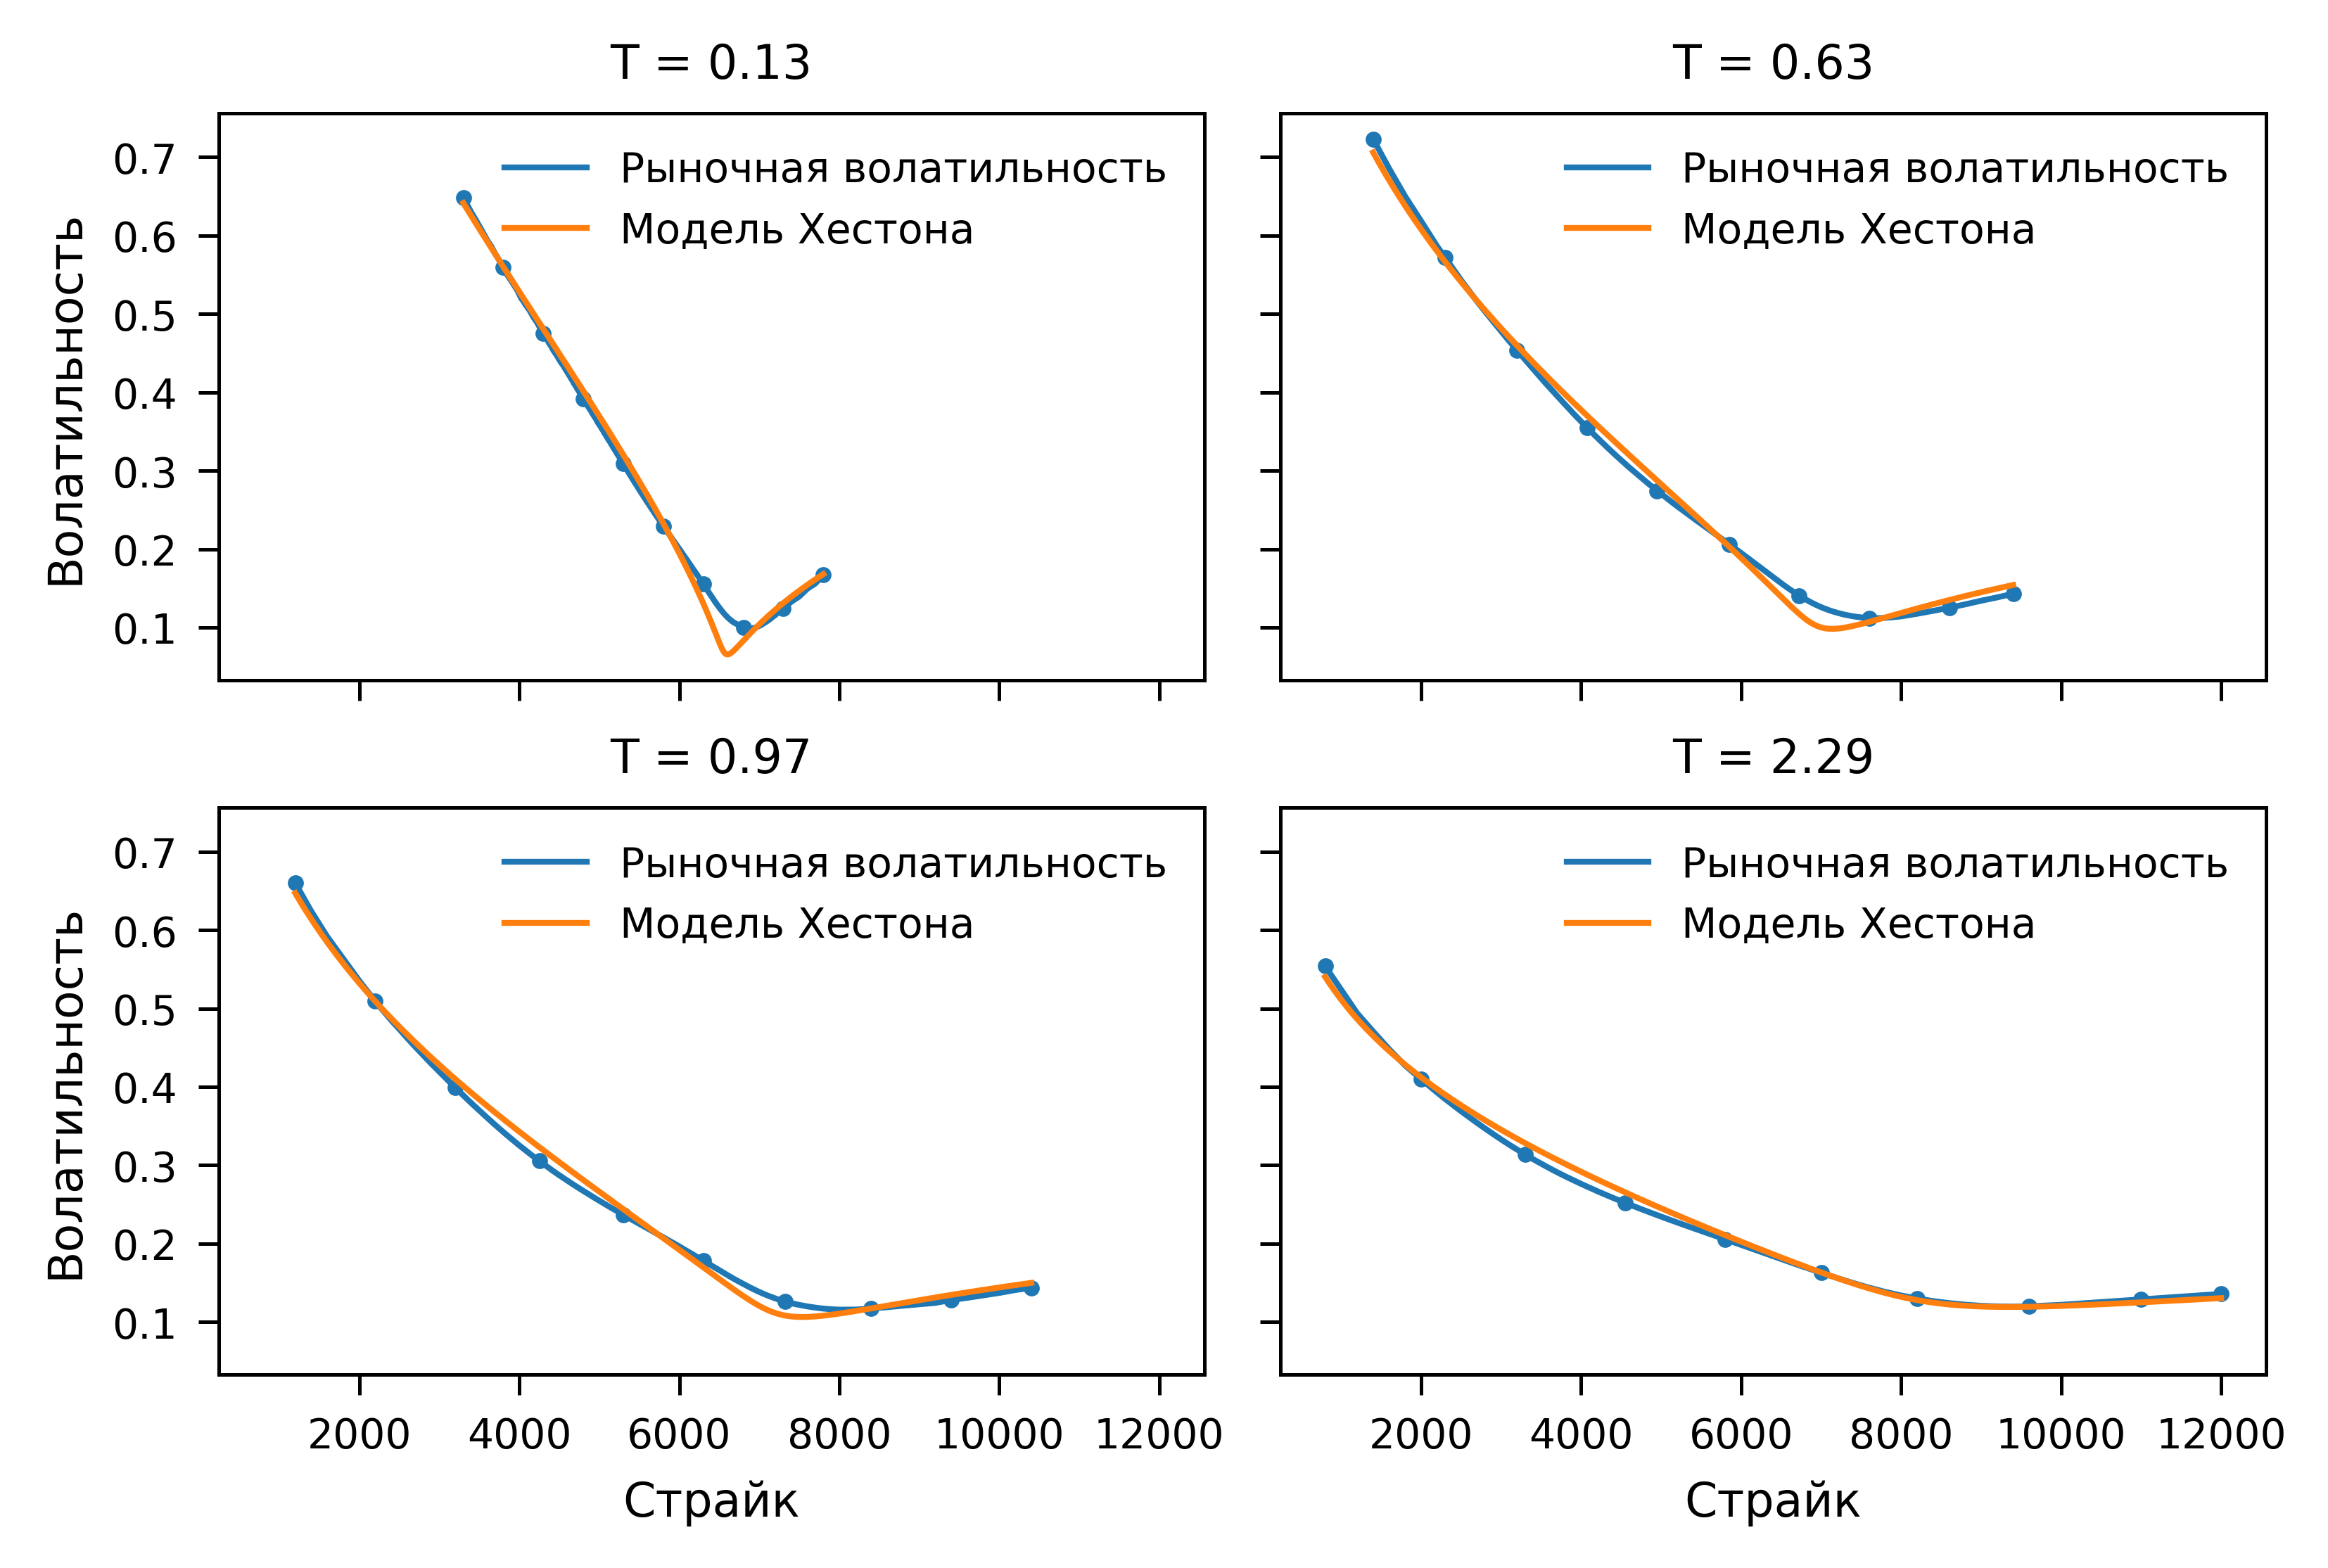
\includegraphics{pic/heston-calibration.png}
\caption{Калибровка модели Хестона к улыбкам волатильности на опционы на индекс SnP 500. Данные на 1.09.2025 г.}
\label{hes:f:calibration}
\end{figure}

В заключение покажем, как параметры модели влияют на форму улыбок волатильности.
Для этого рассмотрим исходную модель с начальной ценой $S_0=1$ и параметрами
\[
V_0=0.09, \quad \kappa=2, \quad \theta=0.09,\quad  \sigma=1, \quad \rho=-0.5
\]
и посмотрим, как будут изменяться улыбки волатильности для времен исполнения $T=0.5$ и $T=2$ при изменении одного из параметров модели.
Результаты представлены на рис.~\ref{hes:f:smiles}.
Из него качественно можно сделать следующие выводы.
\begin{itemize}
\item Параметры $V_0$ и $\theta$, главным образом, отвечают за вертикальное положение улыбок волатильности, причем  $V_0$ больше влияет на улыбки с близким сроком исполнения, а $\theta$ "--- с дальним.
При увеличении этих параметров улыбки смещаются вверх.
\item Параметры $\kappa$ и $\sigma$, главным образом,  отвечает за выпуклость улыбок.
При увеличении $\kappa$ улыбки становятся более выпуклыми, а при увеличении $\sigma$ более плоскими.
\item Параметр $\rho$, главным образом, отвечает за наклон улыбок. Чем меньше его значение, тем более крутой левый хвост имеет улыбка. 
\end{itemize}

\begin{figure}[h!]
\centering
  \begin{subfigure}{\textwidth}
    \centering
    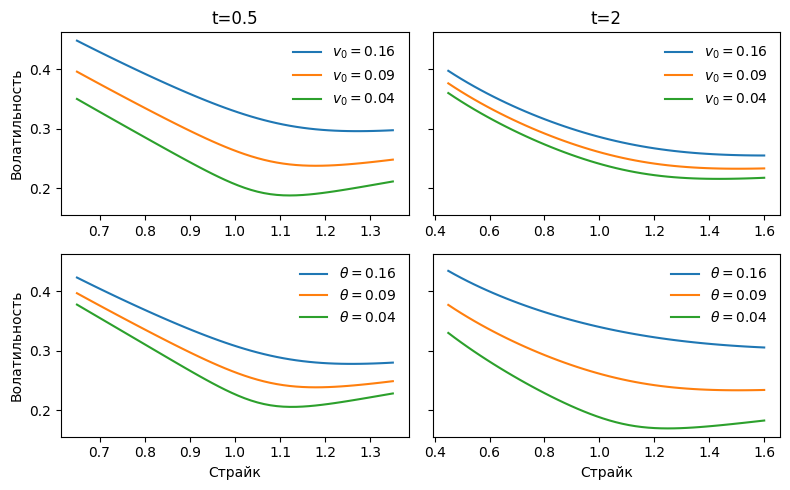
\includegraphics{pic/heston-v0-theta.png}
    \caption{$V_0$ и $\theta$ влияют на вертикальное положение.}
    \label{hes:f:v0-theta}
  \end{subfigure}
  \begin{subfigure}{\textwidth}
    \centering
    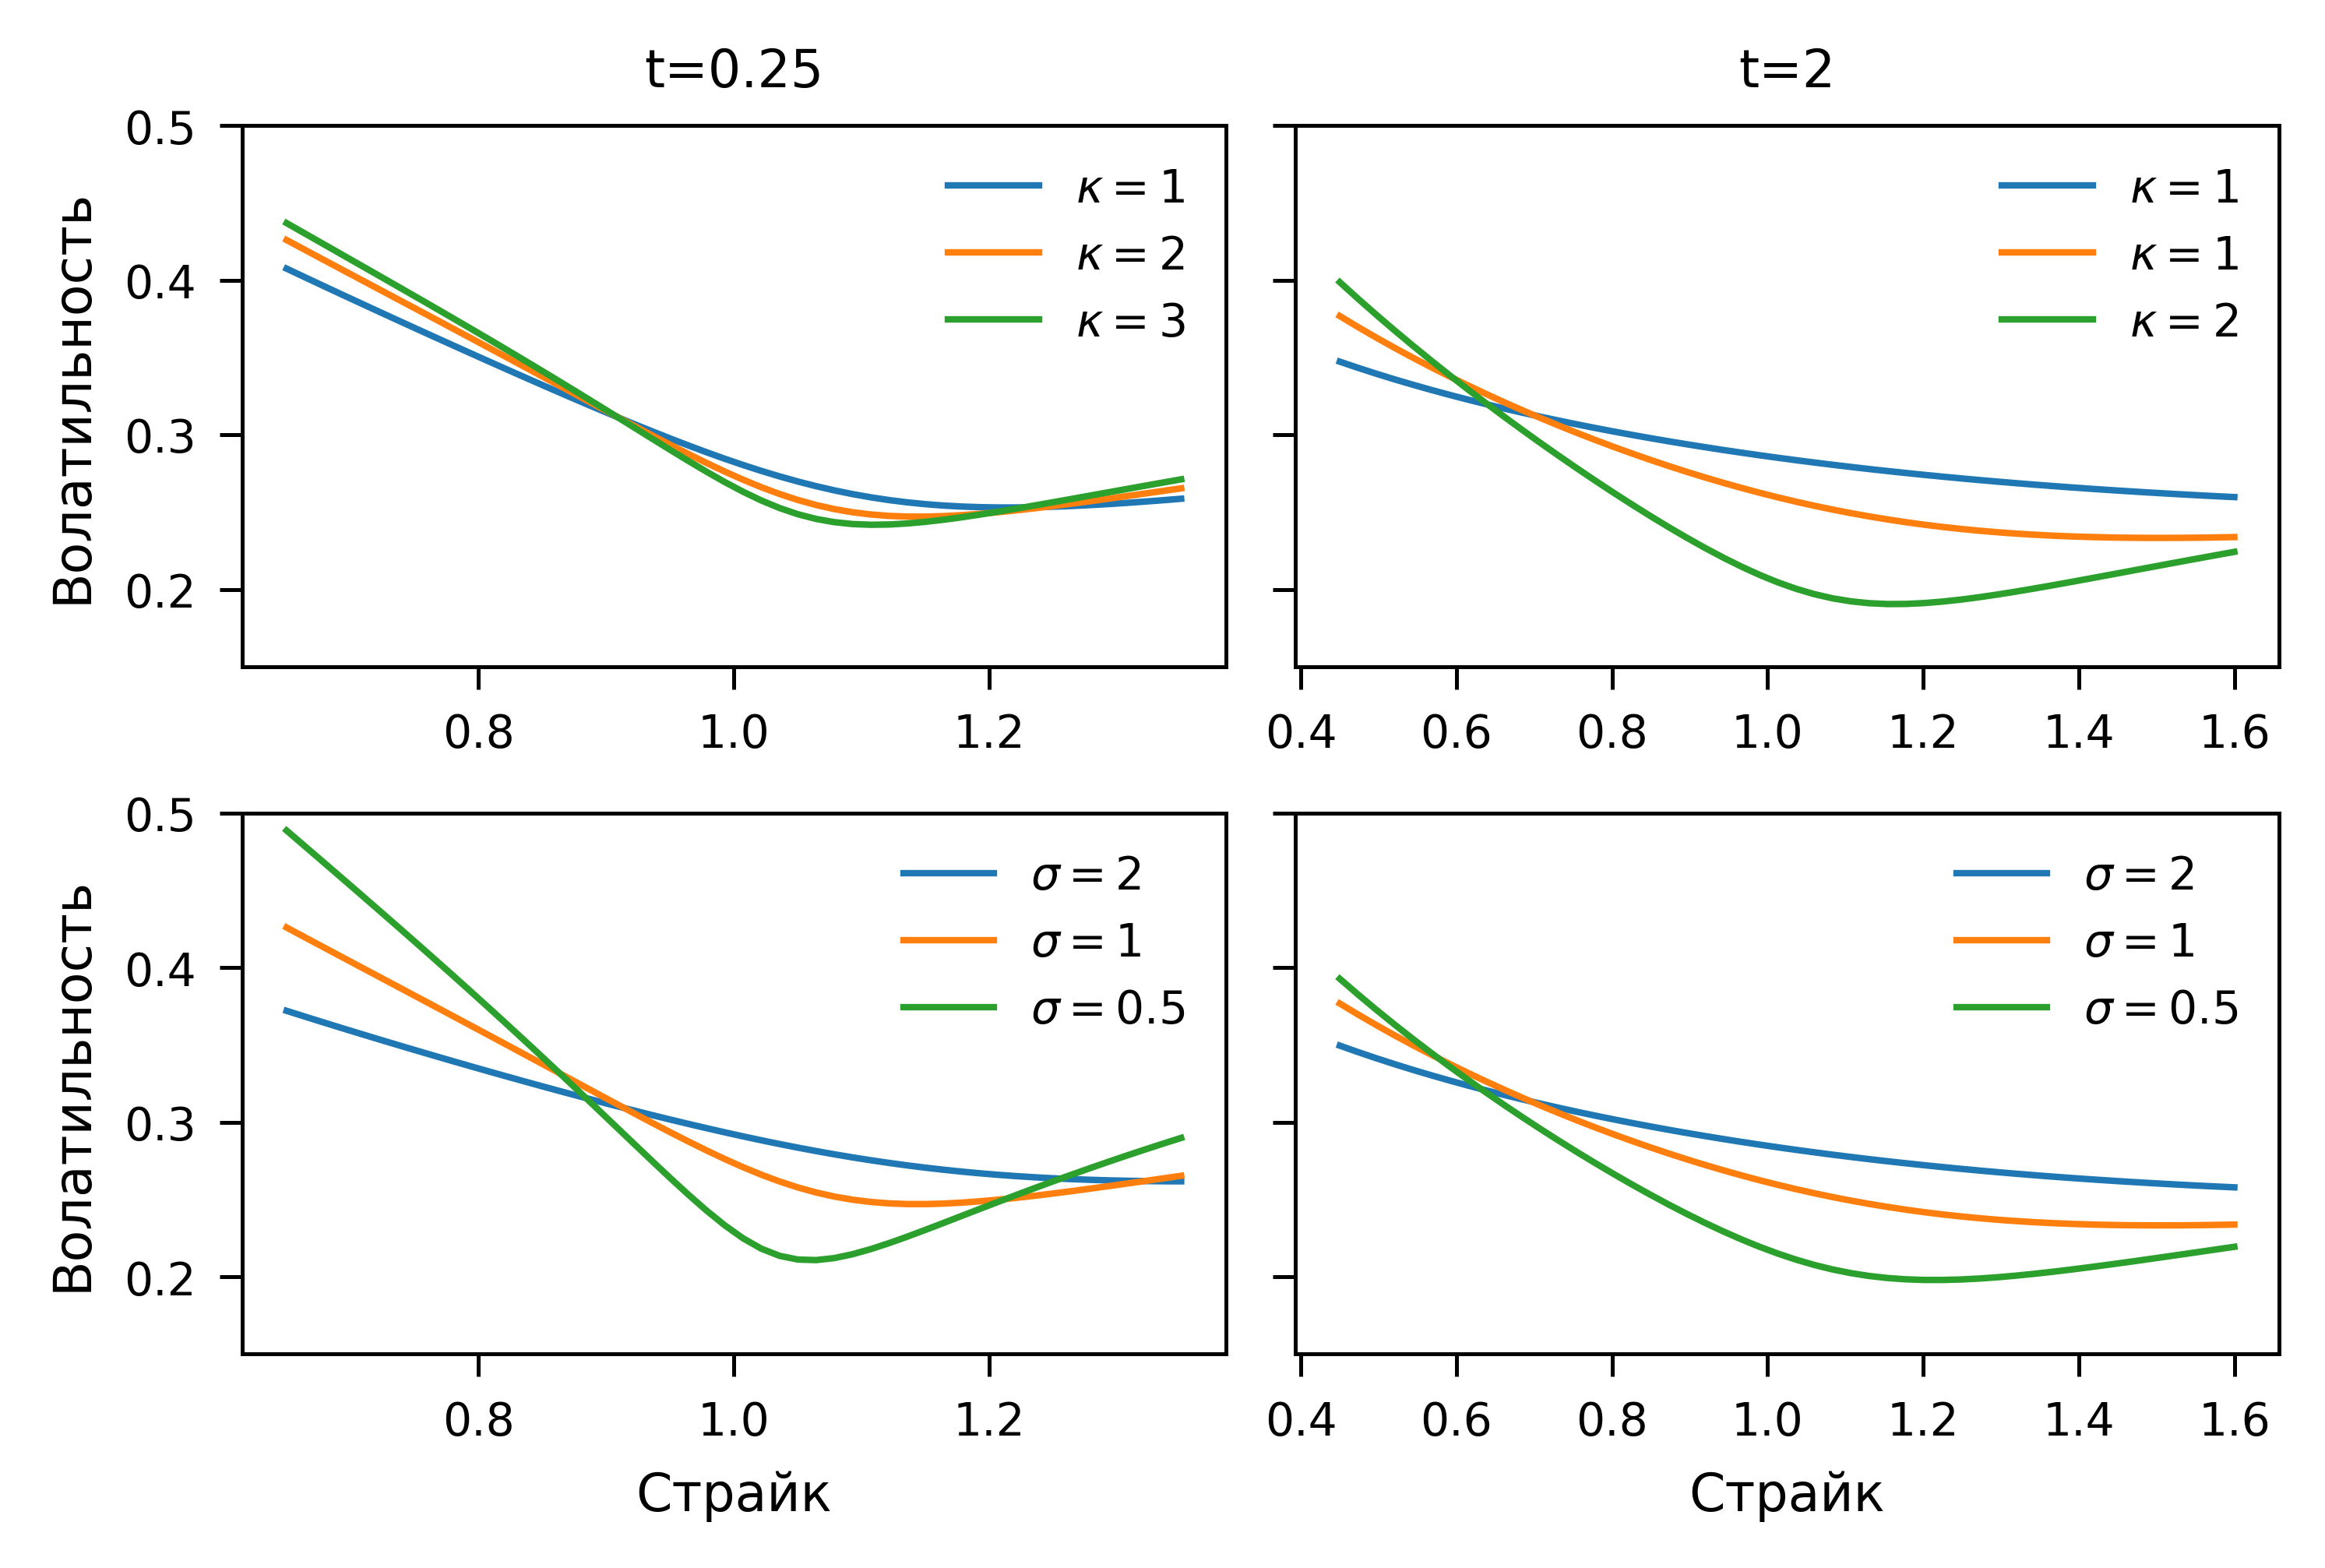
\includegraphics{pic/heston-kappa-sigma.png}
    \caption{$\kappa$ и $\sigma$ влияют на выпуклость.}
    \label{hes:f:kappa-sigma}
  \end{subfigure}
  \begin{subfigure}{\textwidth}
    \centering
    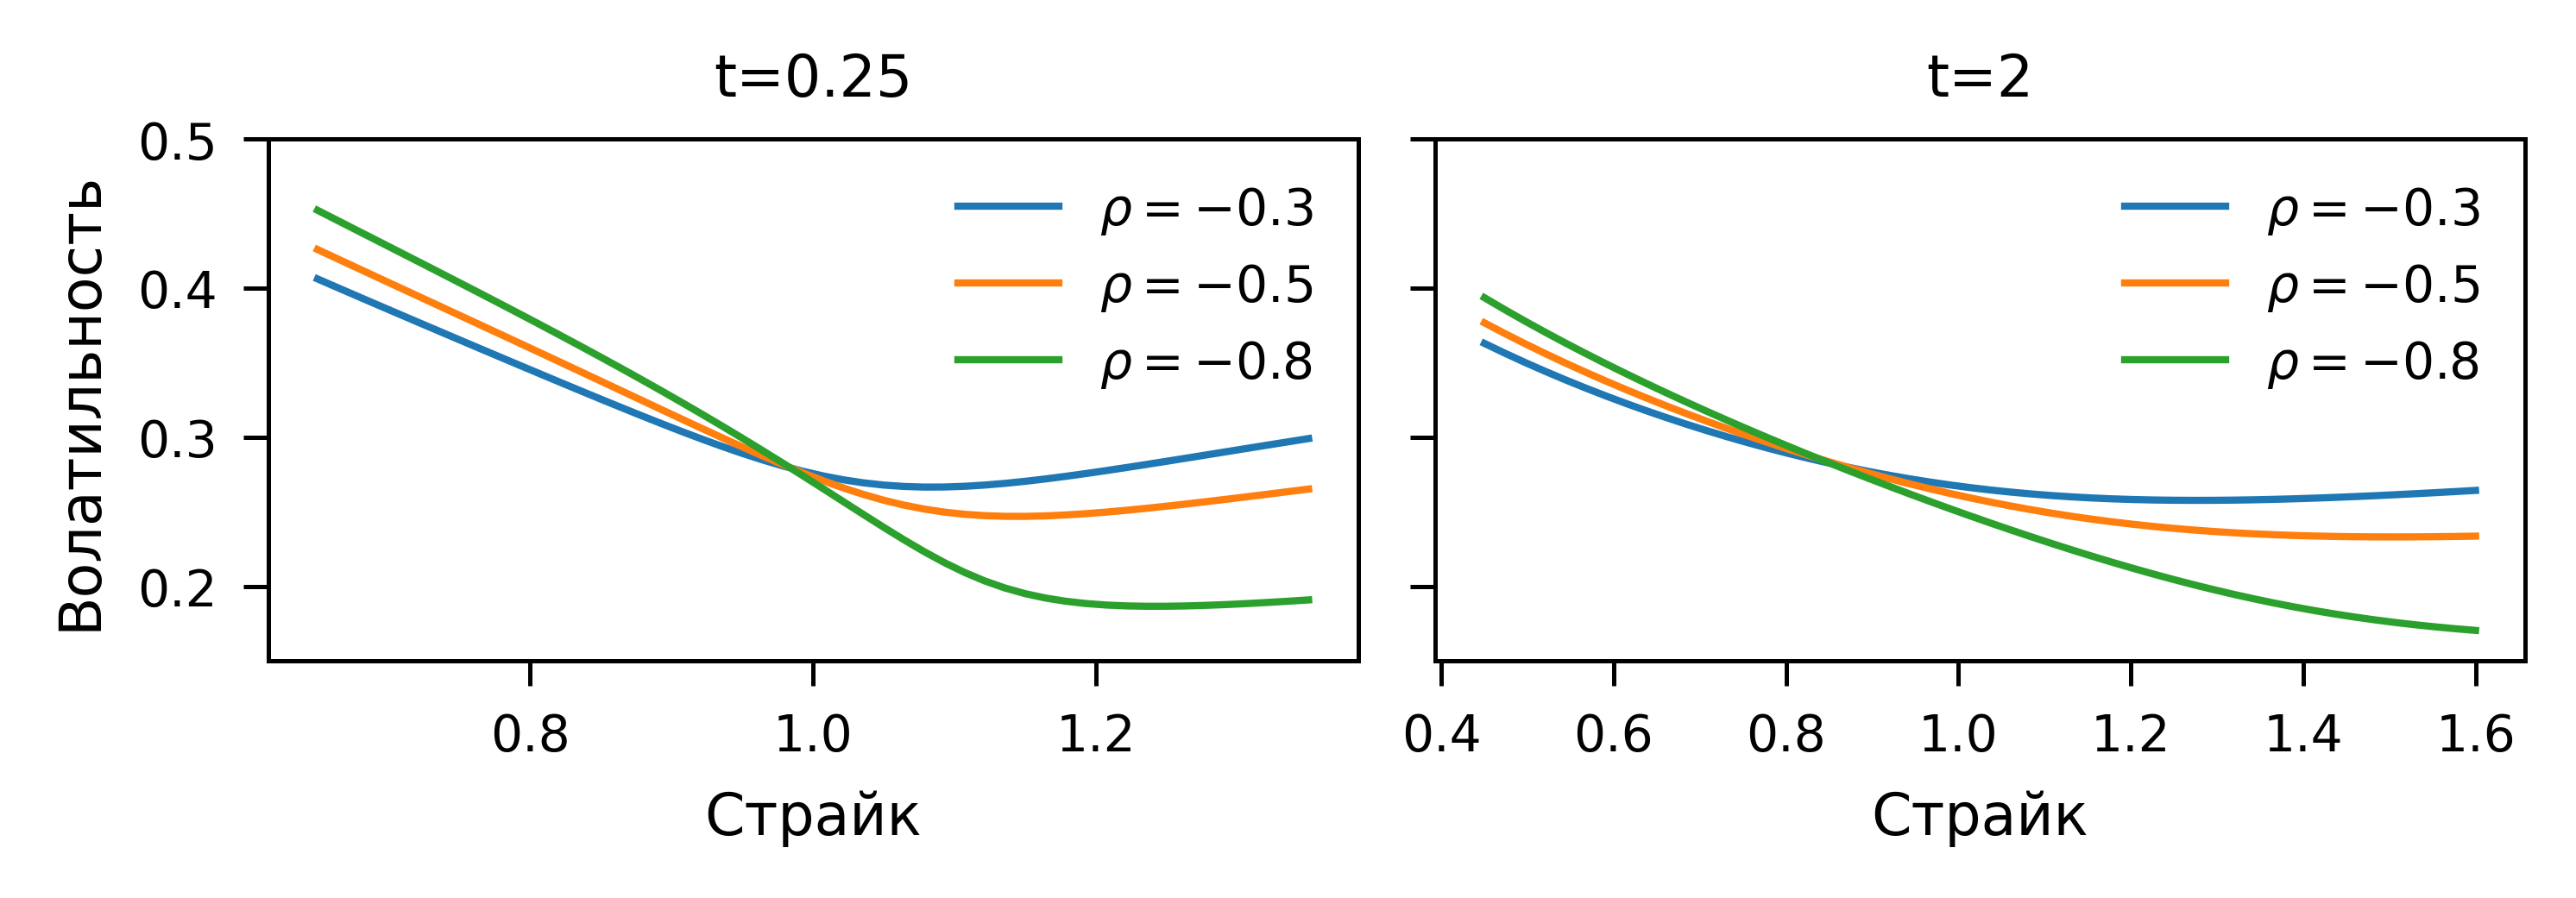
\includegraphics{pic/heston-rho.png}
    \caption{$\rho$ влияет на наклон.}
    \label{hes:f:rho}
  \end{subfigure}
\caption{Влияние параметров модели Хестона на улыбки волатильности.}
\label{hes:f:smiles}
\end{figure}


\summary
\begin{itemize}
\item В модели Хестона стохастическая волатильность задается квадратным корнем процесса CIR. 
\item Стохастическая волатильность строго положительна при выполнении условия Феллера $2\kappa\theta\ge\sigma^2$.
\item Основным результатом лекции является формула для цены европейских опционов колл и пут, сводящаяся к вычислению некоторого интеграла, включающего характеристическую функцию логарифма цены.
Характеристическая функция представима в явном виде.
\item Калибровка (\te\ подбор параметров) модели Хестона обычно осуществляется путем минимизации среднеквадратичного отклонения подразумеваемых волатильностей в модели от рыночных подразумеваемых волатильностей.
\end{itemize}

%!TEX root=finmath2.tex

\chapter{Репликация и оценка производных инструментов в модели Хестона}
\label{ch:hedging}
\chaptertoc

В этой лекции мы получим уравнение с частными производными для цены платежного обязательства в модели Хестона, аналогичное уравнению \bs, а также покажем, как можно реплицировать платежные обязательства, если разрешить включать в портфель дополнительные инструменты.
В третьей части лекции обсуждается метод \mc.

Несмотря на то, что все теория здесь излагается для модели Хестона, общие идеи легко переносятся на другие модели стохастической волатильности.


\section{Уравнение для цены платежного обязательства}

Рассмотрим модель Хестона и будем предполагать, что исходная вероятностная мера уже является мартингальной.
Пусть $r_t$ и $q_t$ "--- безрисковая ставка и ставка дивидендной доходности (обе детерминированные).
Тогда модель задается уравнениями
\begin{align*}
&d S_t = (r_t-q_t) S_t dt + \sqrt{V_t} S_t dW_t^{(1)},\\
&d V_t = \kappa(\theta-V_t) dt + \sigma \sqrt{V_t} dW_t^{(2)},
\end{align*}
где броуновские движения $W^{(1)}$ и $W^{(2)}$ коррелированны с коэффициентом корреляции $\rho$.

Рассмотрим платежное обязательство с выплатой $f(S_T)$.
Напомним, что инструменты с выплатой такого вида называются \emph{независящими от траектории цены базового актива}. 
Будем считать, что функция $f(s)$ ограничена снизу и $\E f(S_T) < \infty$.
Тогда безарбитражная цена этого обязательства равна
\[
U_t = e^{-\int_t^T r_s ds} \E(f(S_T) \mid \F_t),
\]
и, в силу марковского свойства процесса $(S_t,V_t)$, представима в виде $U_t = U(t,S_t,V_t)$ с функцией 
\[
U(t,s,v) = e^{-\int_t^T r_s ds} \E(f(S_T)\mid S_t=s, V_t=v).
\]

Пусть функции $r_t$, $q_t$ и $f(s)$ являются достаточно <<хорошими>>, так что к $U(t,s,v)$ применима формула \fc\ (см.~замечание \ref{sde:r:fc} в лекции \ref{ch:sde}).
Тогда получаем следующее утверждение.

\begin{proposition}
Функция $U(t,s,v)$ удовлетворяет уравнению с частными производными
\begin{align}
\label{hdg:pde}
&\prt Ut + (r_t-q_t)s\prt Us + \kappa(\theta-v)\prt Uv + \frac 12 s^2v \prtt Us + \frac12 \sigma^2v \prtt Uv + \sigma sv \Prtt Usv = r_t U,\\
\label{hgd:pde-boundary}
&U(T,s,v) = f(s).
\end{align}
\end{proposition}

Доказательство непосредственно следует из формулы \fc, применяемой к двумерному процессу $X_t=(S_t,V_t)$, который удовлетворяет уравнению $dX_t = a(t, X_t)dt + b(X_t) dW_t$ с двумерным броуновским движением $W_t = (W_t^{(1)}, W_t^{(2)})$ и коэффициентами
\[
a(t,s,v) = ((r_t-q_t)s,\ \kappa(\theta-v)), \qquad b(s,v) = (s\sqrt{v},\ \sigma\sqrt{v}).
\]

Уравнение \eqref{hdg:pde} можно решать численно методом конечных разностей.
Однако по сравнению, например, с уравнением \bs, в котором функция цены зависит только от двух переменных $(t,s)$, здесь задача становится более трудной.
Во первых, из-за присутствия трех измерений возрастает число узлов сетки, в которых вычисляется функция $U$.
Во-вторых, для неявной схемы или схемы Кранка"--~Николсона не получается применить метод прогонки, так как получаемые на каждом шаге системы линейных уравнений не являются трехдиагональными.
Если же пользоваться обычными методами решения линейных систем, то количество операций резко возрастает (напомним: для метода прогонки оно растет линейно с ростом размера матрицы, а в общем случае кубически).
В дополнении \ref{ch:adi} изложен \emph{метод чередования направлений}, который позволяет уменьшить вычислительную сложность задачи.


\section{Реплицирующие стратегии}
Так как модель Хестона не полна, то, вообще говоря, платежные обязательства в ней нельзя реплицировать портфелями, состоящими только из рискового и безрискового актива (см.~пояснение в разделе \ref{gen:s:complete} лекции \ref{ch:general}).
Репликация становится возможной, если добавить в портфель другие производные инструменты.
Покажем, как это сделать.

Нам потребуется многомерный вариант теоремы о мартингальном представлении (подробнее про теорему о мартингальном представлении в одномерном случае см.~лекцию 9 курса \intro).

\begin{proposition}[теорема о мартингальном представлении, см.~\cite{Kallenberg97}, гл.~16, теорема 16.10]
Пусть на пространстве $(\Omega, \F, \FF, \P)$ задано $d$-мерное броуновское движение $W=(W_t)_{t\ge0}$ (возможно, с коррелированными компонентами), а фильтрация $\FF$ порождена им и пополнена.
Тогда для любого локального мартингала $M = (M_t)_{t\ge 0}$ найдется $d$-мерный процесс $H$ такой, что \as\ для всех $t\ge 0$ выполнено равенство
\[
M_t = M_0 + \sum_{i=1}^d \int_0^t H_s^{(i)} d W_s^{(i)},
\]
причем стохастические интегралы корректно определены. 

Если корреляционная матрица процесса $W$ постоянна и невырождена, то процесс $H$ единственен $\P\otimes\mathrm{Leb}$-\as
\end{proposition}

В модели Хестона, как и выше, будем предполагать, что исходная вероятностная мера уже является мартингальной.
Рассмотрим ограниченное снизу платежное обязательство $X$ такое, что $\E X < \infty$.
Тогда по теореме о мартингальном представлении его дисконтированная цена $\tilde C_t = B_T^{-1}\E(X \mid \F_t)$ имеет стохастический дифференциал
\[
d \tilde C_t = a_t^{(1)} dW_t^{(1)} + a_t^{(2)} dW_t^{(2)}.
\]

Пусть помимо безрискового и рискового актива есть возможность включить в реплицирующий портфель дополнительное платежное обязательство $Y$, дисконтированная цена которого $\tilde U_t$ представима в таком же виде:
\[
d \tilde U_t = b_t^{(1)} dW_t^{(1)} + b_t^{(2)} dW_t^{(2)},
\]
причем $b_t^{(2)} \neq 0$. 
Тогда процесс дисконтированной стоимости самофинансируемого портфеля $\pi_t = (G_t, H_t, L_t)$, где $L_t$ "--- количество единиц обязательства $Y$, имеет стохастический дифференциал
\[
d \tilde V_t^\pi = H_t d\tilde S_t + L_t d \tilde U_t = (H_t\sqrt{V_t} \tilde S_t + L_tb_t^{(1)}) d W_t^{(1)} + L_tb_t^{(2)} dW_t^{(2)}.
\]
Положим $V_0^\pi = C_0$ и
\begin{equation}
\label{hdg:LH}
L_t = \frac{a_t^{(2)}}{b_t^{(2)}}, \qquad H_t = \frac{a_t^{(1)} - L_tb_t^{(1)}}{\sqrt{V_t} \tilde S_t}.
\end{equation}
%TODO Пояснить, что знаменатель H_t может обращаться в 0 не более, чем на пренебрежимом множестве
Тогда $d\tilde V_T^\pi = d\tilde C_t$ и, следовательно, 
процессы $\tilde V_t^\pi$ и $\tilde U_t$ совпадают.
Таким образом, $\pi_t=(G_t,H_t,L_t)$, где $G_t = (V_t^\pi - H_t S_t - L_t C_t)/B_t$, является допустимой самофинансируемой стратегией, реплицирующей платежное обязательство $X$ (допустимость следует из предположения об ограниченности выплаты снизу).

Формула \eqref{hdg:LH} задает реплицирующую стратегию в общем виде.
Отдельно рассмотрим частный случай, когда $X$ и $Y$ не зависят от траектории цены базового актива. 
Тогда, аналогично рассуждениям в предыдущем разделе, имеем $\tilde C_t = B_{T}^{-1} C(t,S_t,V_t)$, $\tilde U_t = B_{T}^{-1} U(t,S_t,V_t)$, и из применения формулы Ито следует, что 
\begin{gather*}
a_t^{(1)} = \tilde C'_s(t,S_t,V_t) \sqrt{V_t}S_t, \qquad
a_t^{(2)} = \sigma \tilde C'_v(t,S_t,V_t)\sqrt{V_t},\\
b_t^{(1)} = \tilde U'_s(t,S_t,V_t) \sqrt{V_t}S_t, \qquad
b_t^{(2)} = \sigma \tilde U'_v(t,S_t,V_t)\sqrt{V_t}.
\end{gather*}
Тогда из формулы \eqref{hdg:LH}, после сокращения дисконтирующих множителей, получаем $L_t = L(t,S_t,V_t)$, $H_t = H(t,S_t,V_t)$ с функциями
\[
L = \frac{U'_v}{C'_v}, \qquad 
H = U'_s - L C'_s.
\]


\section{Метод \mc}
\subsection{Общие принципы}
Метод \mc\ является универсальным инструментом для вычисления математических ожиданий случайных величин с помощью симуляции. 
В частности, его можно применять для оценки цен европейских обязательств по формуле
\[
V = B_T^{-1}\E^{\Q} X.
\]

Основные идеи метода \mc\ были рассмотрены в курсе \intro\ (лекция~14). 
Здесь мы обсудим особенности его применения в моделях стохастической волатильности, где, как правило, отсутствуют простые способы симуляции траекторий в точности из распределения процесса цены, а доступны лишь приближенные методы.

Будем рассматривать задачу оценки платежного обязательства с выплатой $X=f(S_{T_1},\dots, S_{T_m})$ в момент времени $T\ge T_m$. 
Согласно методу \mc, необходимо получить $n$ траекторий процесса цены, где $i$-я траектория представлена набором значений $s_{T_1}^i, \dots, s_{T_m}^i$ в точках $T_1,\dots,T_m$, и аппроксимировать
\[
\E X \approx \frac1n \sum_{i=1}^n f(s_{T_1}^i, \dots, s_{T_m}^i), \qquad n\to\infty.
\]
Эта аппроксимация основана на законе больших чисел: при $n\to\infty$ правая часть сходится к $\E X$, при условии, что $\E X<\infty$.

Возникает вопрос: как получить значения $s_{T_1}^i, \dots, s_{T_m}^i$?  
Далее мы опишем наиболее простую схему симуляции случайных процессов "--- \emph{схему Эйлера} и ее модификацию для модели Хестона.

В общем виде схема Эйлера предназначена для аппроксимации решений стохастических дифференциальных уравнений. 
Пусть требуется получить траекторию процесса, являющегося решением уравнения
\begin{equation}
\label{hdg:mc-sde}
d X_t = a(t,X_t) dt + b(t,X_t) dW_t, \qquad X_0 = x_0,
\end{equation}
где процессы $X_t$ и $W_t$ в общем случае многомерны; $W_t$ "--- броуновское движение с нулевым средним и корреляционной матрицей $\Sigma=(\sigma_{ij})_{i,j=1}^d$, то есть $\E W_t^i W_t^j = \sigma_{ij} t$. 
Будем предполагать, что уравнение имеет единственное сильное решение.

\emph{Дискретизируем} уравнение \eqref{hdg:mc-sde} "--- выберем достаточно малый шаг $\Delta t$ и рассмотрим точки $t_i=i\Delta t$ (возможна и неравномерная сетка; рассуждения остаются теми же). 
Если выплата зависит от значений цены в моментах $T_j$, необходимо включить все $T_j$ в множество узлов $t_i$. 
Обычно берут более плотную сетку, чем точки $T_j$, чтобы уменьшить ошибку дискретизации.

Значения $X_{t_i}$ симулируются последовательно.
Если известно $\hat X_{t_i}$, то полагают
\[
\hat X_{t_{i+1}} = \hat X_{t_i} + a(t_i,\hat X_{t_i})\Delta t + b(t_i,\hat X_{t_i})\Delta W_{t_{i+1}},
\]
где $\Delta W_{t_{i+1}}$ "--- реализация нормального вектора с распределением $\mathcal{N}(0, \Sigma \Delta t)$.
Эта схема основана на интегральном представлении
\[
X_{t_{i+1}} = X_{t_i} + \int_{t_i}^{t_{i+1}} a(u,X_u)\,du + \int_{t_i}^{t_{i+1}} b(u,X_u)\,dW_u,
\]
в котором подынтегральные выражения аппроксимируются значениями в левом конце отрезка интегрирования.

Надстрочные <<крышки>> в обозначениях мы будем использовать, чтобы различать случайные величины, полученных по схеме Эйлера, от истинных значений процесса $X_t$ (векторы $(X_{t_i})_{i=1}^m$ и $(\hat X_{t_i})_{i=1}^m$ имеют разные распределения).
При достаточно малом $\Delta t$ их распределения близки, поэтому применяют аппроксимацию
\[
\E f(X_{t_1},\dots, X_{t_m}) \approx \frac1n \sum_{i=1}^n f(\hat X_{t_1}^i,\dots, \hat X_{t_m}^i).
\]
Подробнее о сходимости сказано в разделе \ref{hdg:s:mc-convergence}.


\subsection{Схема Эйлера для модели Хестона}
Перепишем модель Хестона в эквивалентной форме:
\begin{align*}
&d S_t = \sqrt{V_t}\, S_t (\rho\, d W_t^{(1)} + \sqrt{1-\rho^2}\, d W_t^{(2)}),\\
&d V_t = \kappa(\theta - V_t)\,dt + \sigma \sqrt{V_t}\, d W_t^{(1)},
\end{align*}
где $W^{(1)}$ и $W^{(2)}$ "--- независимые броуновские движения. Нетрудно проверить, что $\rho W_t^{(1)} + \sqrt{1-\rho^2} W_t^{(2)}$ является стандартными броуновскими движениями, коррелированным с $W_t^{(1)}$ с коэффициентом корреляции $\rho$, поэтому данная форма модели эквивалентна исходной.
Такой приём часто используется, так как работать с независимыми броуновскими движениями проще.

\begin{remark}
Если требуется симулировать процесс
\[
d S_t = \mu_t S_t dt + \sqrt{V_t} S_t d W_t,
\]
где $\mu_t$ "--- детерминированный снос, то в схему можно добавить член $\mu_t \Delta t$, либо сначала смоделировать процесс с нулевым сносом, а затем умножить траектории на $e^{\int_0^t \mu_s ds}$.
\end{remark}

Прямое применение схемы Эйлера к системе $(S_t,V_t)$ приводит к проблеме: значения $S_t$ и $V_t$ могут стать отрицательными\footnote{Так как $\Delta W_t^{(1)}$ и $\Delta W_t^{(2)}$ имеют нормальное распределение и могут принимать произвольно большие отрицательные значения.}. 
Чтобы этого избежать, применяют модификацию: вводят $X_t=\ln S_t$ и симулируют систему
\begin{align*}
&\hat X_{t_{i+1}} = \hat X_{t_i} 
  - \frac12 \hat V_{t_i}^+ \Delta t 
  + \sqrt{\hat V_{t_i}^+} 
    \bigl(\rho \Delta W_{t_{i+1}}^{(1)} + \sqrt{1-\rho^2}\, \Delta W_{t_{i+1}}^{(2)}\bigr), \\
&\hat V_{t_{i+1}} = \hat V_{t_i} + \kappa(\theta - \hat V_{t_i}^+)\Delta t 
  + \sigma \sqrt{\hat V_{t_i}^+}\, \Delta W_{t_{i+1}}^{(1)},\\
&\hat S_{t_{i+1}} = \exp(\hat X_{t_{i+1}}).
\end{align*}
Эта схема основана на представлении
\begin{align*}
&d X_t = -\tfrac12 V_t\, dt + \sqrt{V_t^+}\, (\rho\, d W_t^{(1)} + \sqrt{1-\rho^2}\, d W_t^{(2)}),\\
&d V_t = \kappa(\theta - V_t^+)\, dt + \sigma \sqrt{V_t^+}\, d W_t^{(1)},
\end{align*}
где уравнение для $X_t$ получается из уравнения для $S_t$ по формуле Ито. Взятие положительной части не меняет модель, так как $V_t\ge0$.


\subsection{Сходимость схемы Эйлера}
\label{hdg:s:mc-convergence}
Под сходимостью схемы дискретизации стохастического дифференциального уравнения понимают сходимость векторов $(\hat X_{t_1},\dots,\hat X_{t_m})$ к $(X_{t_1},\dots,X_{t_m})$, то есть сходимость аппроксимированных значений к истинным. Важна не только сама сходимость, но и её скорость.

Различают два типа сходимости. Пусть $X_t$ "--- решение СДУ, а $\hat X_t$ "--- его дискретизация (например, по схеме Эйлера).
Зафиксируем момент времени $T$.

\begin{itemize}
\item Говорят, что схема имеет \emph{сильный порядок сходимости $p$}, если
\[
\E |X_T(W) - \hat X_T(W; \Delta t)| = O((\Delta t)^p)\ \text{при}\ \Delta t\to0,
\]
где $X_T(W)$ "--- истинное значение процесса в момент $T$, а $\hat X_T(W;\Delta t)$ "--- его аппроксимация, построенная по приращениям того же броуновского движения.
\item Говорят, что схема имеет \emph{слабый порядок сходимости $p$}, если
\[
\E f(X_T) - \E f(\hat X_T(\Delta t)) = O((\Delta t)^p)\ \text{при}\ \Delta t\to0,
\]
для любой функции $f$ из некоторого класса функций, удовлетворяющих определенным условиям гладкости. Здесь неважно, по каким броуновским движениям строятся процесс и его аппроксимация.
\end{itemize}

Различие понятий сильного и слабого порядка состоит в том, что сильный порядок отвечает за <<потраекторную>> близость, а слабый "--- лишь за близость математических ожиданий функций от процесса. В приложениях к оценке деривативов более релевантно понятие слабого порядка сходимости, так как для вычисления цен требуется именно вычислять математические ожидания.

\begin{proposition}
Если коэффициенты рассматриваемого СДУ удовлетворяют некоторым условиям регулярности, то схема Эйлера имеет сильный порядок сходимости $1/2$ и слабый порядок сходимости $1$ (для достаточно гладких функций $f$).
\end{proposition}

Точные формулировки условий можно найти, например, в книге \cite{KloedenPlaten95}: теорема 10.2.2 для сильного порядка и теоремы 14.1.6, 14.5.2 для слабого порядка.

На практике шаг $\Delta t$ можно выбирать следующими способами: либо уменьшать $\Delta t$, пока различие между результатами для двух последовательных значений $\Delta t$ не станет достаточно малым, либо подобрать такое значение, что для инструментов, цены которых можно найти аналитически, достигалась заданная точность.

Таким образом, при применении метода \mc\ для вычисления цен платежных обязательств возникают две ошибки: ошибка самого метода \mc, связанная с заменой математического ожидания на среднее по выборке, и ошибка дискретизации, возникающая из-за того, что вместо настоящего решения стохастического дифференциального уравнения используется его дискретная аппроксимация.

На рис.~\ref{hdg:f:euler} проиллюстрирована ошибка дискретизации в схеме Эйлера. 
Графики показывают отклонение подразумеваемой волатильности, когда цены опционов вычисляются по методу \mc\ с помощью схемы Эйлера, от истинной подразумеваемой волатильности (мы сравниваем подразумеваемые волатильности, а не цены опционов, так как они более информативны).
Время до исполнения опционов на графиках $T=1$ год.

В дополнении \ref{ch:qe} будет описана другая схема аппроксимации "--- схема QE, которая позволяет обойтись существенно меньшим количеством промежуточных точек для достижения хорошей точности.

\begin{figure}[th]
\centering
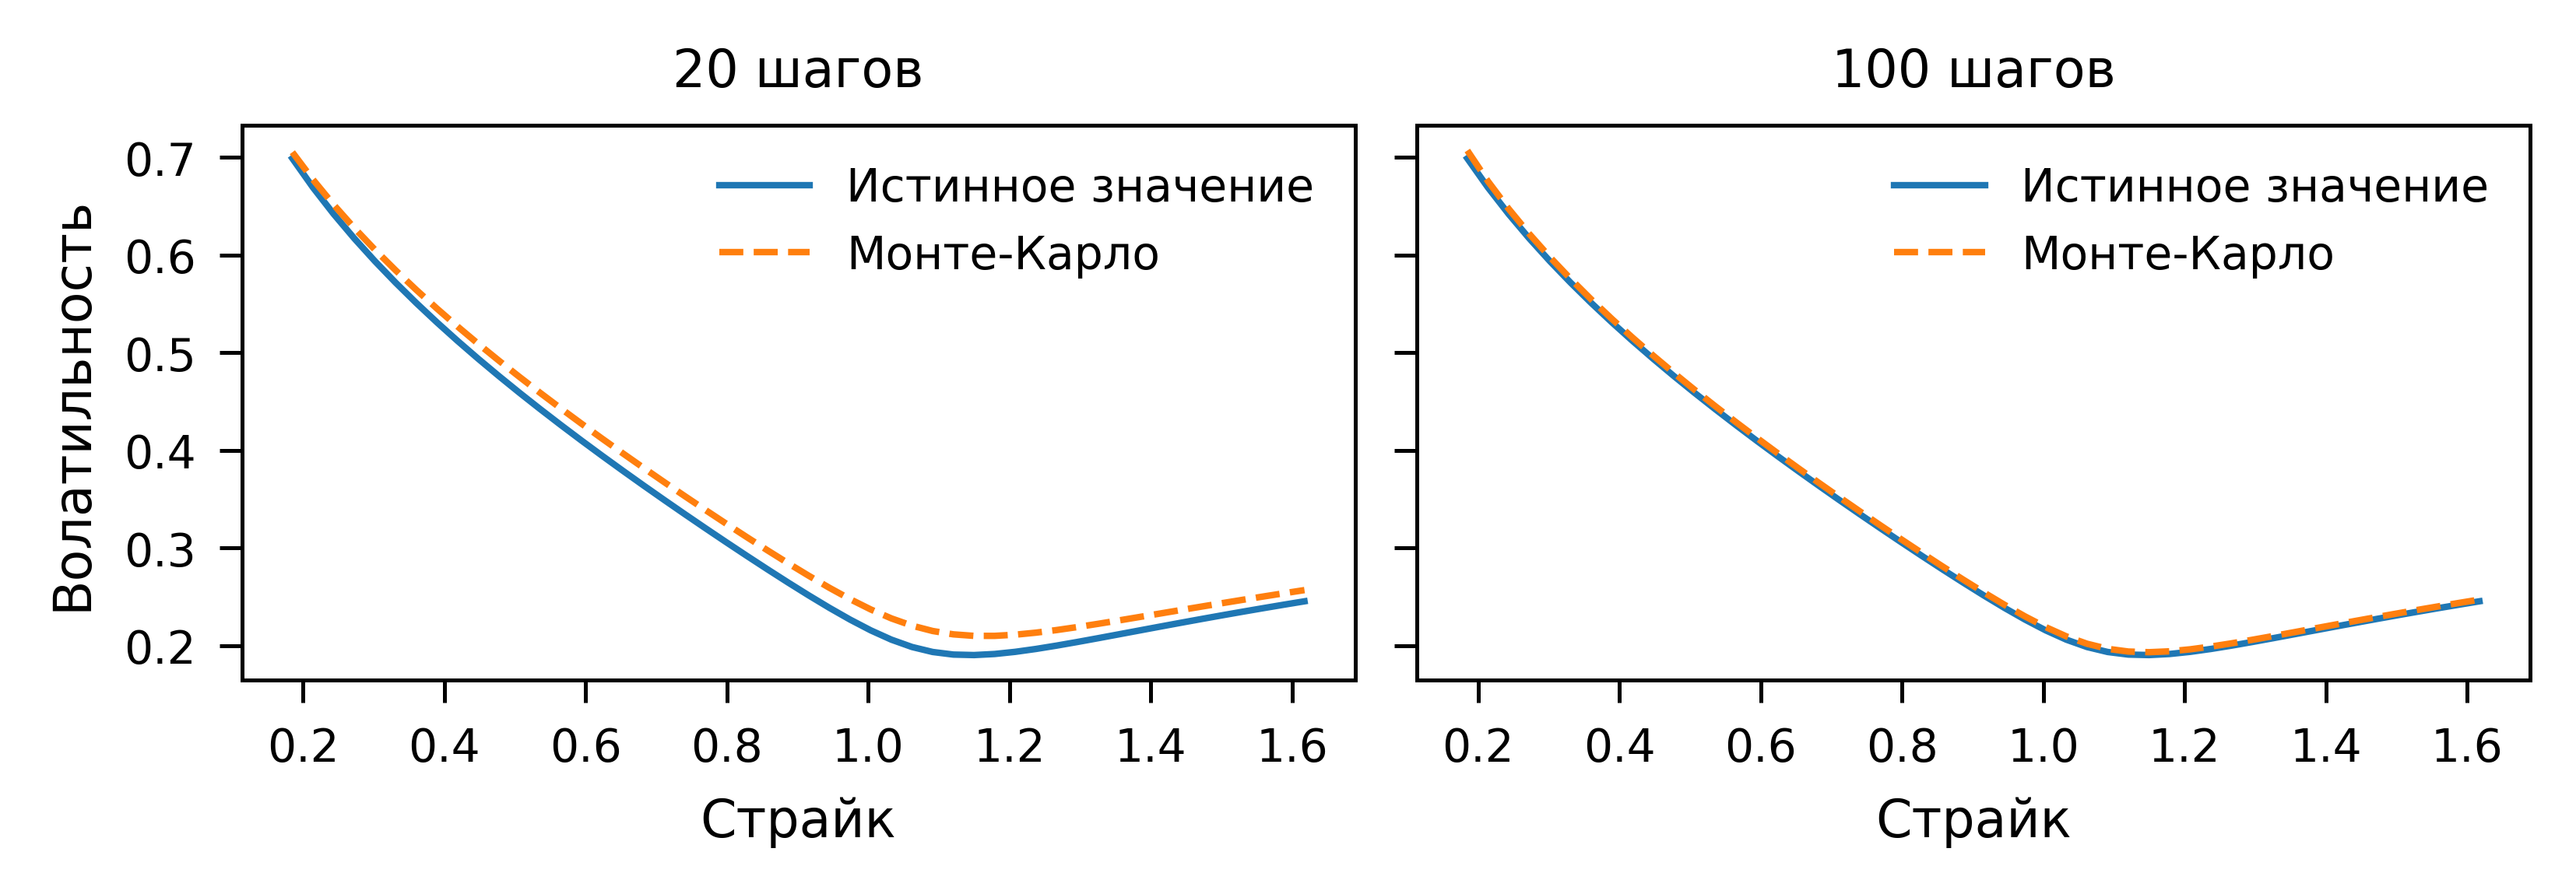
\includegraphics{pic/heston-euler.png}
\caption{Сходимость схемы Эйлера для модели Хестона.}
\label{hdg:f:euler}
\end{figure}


\summary
\begin{itemize}
\item В модели Хестона цены платежных обязательств, не зависящих от траектории цены базового актива, удовлетворяют дифференциальному уравнению с частными производными \eqref{hdg:pde}--\eqref{hgd:pde-boundary}.

\item Становится возможным реплицировать платежные обязательства, если добавить в портфель какое-нибудь дополнительно торгуемое платежное обязательство (например, опцион колл или пут).

\item Цены платежных обязательств можно вычислять с помощью метода \mc.
Для симуляции случайных процессов их траектории нужно дискретизировать.
В лекции рассматривалась схема дискретизации Эйлера.

\item Схема Эйлера имеет сильный порядок сходимости 1/2 и слабый порядок сходимости 1.
\end{itemize}


%!TEX root=finmath2.tex
\stopchaptertoc

\part*{Дополнения к лекциям}
\titleformat{\chapter}[display]{\bfseries\Large}{\underline{Дополнение~\thechapter}}{0.5em}{}
\titlecontents{chapter}[0em]{}{\textbf{Дополнение\ \thecontentslabel.}\hspace{2mm}}{}{\dotfill\contentspage}
\setcounter{chapter}{0}
\renewcommand{\theHchapter}{A\arabic{chapter}}%


\chapter{К модели локальной волатильности}
\label{ch:lv-s}

Здесь собраны результаты о модели локальной волатильности, которые не вошли в лекцию \ref{ch:locvol}, но представляют определенный интерес. 

\section{Формула Дюпира через подразумеваемую волатильность}

Формулу Дюпира для локальной волатильности можно переписать так, чтобы вместо поверхности цен опционов она содержала поверхность \emph{полной подразумеваемой дисперсии}.
Полная подразумеваемая дисперсия опциона (total implied variance) равна величине $\hat w = \hat\sigma^2 T$, где $\hat\sigma$ "--- его подразумеваемая волатильность.
Представление локальной волатильности через $\hat w$ может быть удобно, когда дана поверхность подразумеваемой волатильности, а не непосредственно цены опционов.

Сделаем замену координат и вместо страйка $K$ будем использовать \emph{лог"=форвардную денежность} $y=\ln (K/F_0^T)$, где $F_0^T = B_T S_0$ обозначает $T$"=форвардную цену в момент времени $t=0$.
Величины $S_0$ и функция $B_t$ считаются фиксированными; безрисковая процентная ставка неслучайна.

Нетрудно видеть, что имеется взаимно-однозначное соответствие между переменными $(T,K,\sigma)$ и $(T,y,w)$, причем подразумеваемая волатильность $\hat \sigma(T,K)$ и полная подразумеваемая дисперсия $\hat w(T,y)$ связаны по формулам 
\[
\hat w(T,y) = \hat\sigma^2(T, e^yF_0^T)T, \qquad \hat\sigma(T,K) = \sqrt{\hat w(T,\ln(K/F_0^T))/T}.
\]

\begin{proposition}
Пусть для заданной поверхности цен опционов $\hat C(T,K)$ выполнены условия теоремы \ref{lv:t:dupire} из лекции \ref{ch:locvol}.
Тогда локальную волатильность можно представить в виде $\sigma(t,s) = \sqrt{v(t, \ln(s/F_0^t))}$, где функция $v(t,y)$ связана с $\hat w(t,y)$ по формуле
\begin{equation}
\label{lv:v}
v(t,y) = \frac{\hat w'_T(t,y)}{1 - \frac{y}{\hat w(t,y)} \hat w'_y(t,y) - \frac14\Bigl(\frac14 + \frac1{\hat w(t,y)} - \frac{y^2}{\hat w^2(t,y)}\Bigr)(\hat w'_y(t,y))^2 + \frac12 \hat w''_{yy}(t,y)}.
\end{equation}
\end{proposition}

\begin{proof}
В переменных $(y,w)$ формула Блэка для цены опциона колл принимает вид
\begin{align*}
&c(y, w) = S_0(\Phi(d_1) - e^y \Phi(d_2)),\\
&d_1 = -\frac{y}{\sqrt w}  + \frac{\sqrt{w}}{2}, \qquad d_2 = d_1 - \sqrt w.
\end{align*}
Путем непосредственного дифференцирования проверяются следующие соотношения между производными:
\begin{align*}
%&c'_T = c\,r_T,& & & &\\
&c'_y = c - S_0\Phi(d_1),& &c'_w = \frac{S_0}{2\sqrt w}\phi(d_1),& &\\
&c''_{yy} = c'_y + 2c'_w,& &c''_{wy}= \Bigl(\frac12 - \frac yw\Bigr)c'_w,& 
&c''_{ww} = -\Bigl(\frac18 + \frac1{2w} - \frac{y^2}{2w^2}\Bigr) c'_w,\\
&y'_T = -r_T,& &y'_K = \frac1K,& &y''_{KK} = -\frac1{K^2}.
\end{align*}
Далее в формулу Дюпира
\begin{equation}
\label{lv:dupire-KT}  
\sigma^2(T,K) = 2\frac{\prt{}T C(T,K) + r_TK\prt{}KC(T,K)}{K^2\prtt{}K C(T,K)}
\end{equation}
подставим $C(T,K) = c(y(T,K), \hat w(T, y(T,K)))$ и вычислим производные:
\begin{align*}
\prt CT &=  c'_y y'_T + c'_w(\hat w'_T + \hat w'_y y'_T) = -r_T (c'_y + c'_w \hat w'_y) + c'_w \hat w'_T,\\[0.3em]
\prt CK &= (c'_y + c'_w\hat w'_y) y'_K = (c'_y + c'_w\hat w'_y) \frac1K,\\[0.3em]
\prtt CK &= c''_{yy}(y'_K)^2 + 2 c''_{yw} y'_K \prt wK + c'_y y''_{KK} + c''_{ww}y'_K\prt wK + c'_w \Bigl(\prt wK\Bigr)^2 + c'_w \prtt wK\\[0.3em]
&= \frac2{K^2} c'_w\biggl(1 - \frac yw w'_y -\frac14\Bigl(\frac14 + \frac1w - \frac{y^2}{w^2}\Bigr)(w'_y)^2 + \frac12 w''_{yy}\biggr).
\end{align*}
Из первых двух равенств находим, что
\[
\prt{}T C(T,K) + r_TK\prt{}KC(T,K) = c'_w w'_T.
\]
Подставляя полученные выражения в \eqref{lv:dupire-KT}, получаем формулу \eqref{lv:v}.
\end{proof}




\section{Локальная волатильность форвардной цены}
Покажем, что в модели локальной волатильности форвардная цена тоже допускает представление в виде уравнение, где коэффициент волатильности зависит только от времени и форвардной цены. 

\begin{proposition}
Пусть цена рискового актива задается моделью локальной волатильности $dS_t = r_tS_t dt + \sigma(t,S_t) S_t d W_t$, где процентная ставка $r_t$ неслучайна. Тогда $T$-форвардная цена $F_t^T = S_tB_T/B_t$, где $t\in[0,T]$, удовлетворяет уравнению
\[
d F_t^T = \sigma_f(t,F_t^T) F_t^T d W_t, \qquad F_0^T = S_0B_T,
\]
с функцией
\[
\sigma_f(t,f) = \sigma(t,f B_t/B_T),
\]
а процесс приращения логарифма форвардной цены $Y_t^T = \ln F_t^T - \ln F_0^T$ удовлетворяет уравнению
\[
d Y_t^T = -\frac12 v(t, Y_t^T) dt + \sqrt{v(t, Y_t^T)} d W_t, \qquad X_0^T=0,
\]
где $v(t,y)$ "--- функция из \eqref{lv:v}.
\end{proposition}

\begin{proof}
Как было показано в лекции \ref{ch:general} (см.~следствие \ref{gen:c:forward-vol}), коэффициент волатильности у процессов $F_t$ и $S_t$ одинаковый (в том смысле, что это один и тот же случайный процесс), а коэффициент сноса у $F_t$ нулевой. Таким образом,
\[
d F_t = \sigma(t,S_t)F_t d W_t = \sigma(t, F_tB_t/B_T) F_tdW_t,
\]
что и требовалось доказать.

Чтобы получить уравнение для $Y_t^T$, заметим, что из соотношения $\sigma^2(t,s) = v(t, \ln(s/F_0^t))$ следует, что
\[
\sigma^2_f(t,F_t^T) = \sigma^2(t,F_t^TB_t/B_T) = v(t, \ln(F_t^TB_t/(B_TF_0^t))) = v(t,Y_t^T).
\]
Применяя далее формулу Ито к $Y_t^T$, получаем требуемое уравнение.
\end{proof}


%%%%%%%%%%%%%%%%%%%%%%%%%%%%%%%%%%%%%%%%%%%%%%%%%%%%%%%%%%%%%%%%%%%%%
%%% Этот фрагмент нужно перенести в следующий курс, в материал про LSV
%%%%%%%%%%%%%%%%%%%%%%%%%%%%%%%%%%%%%%%%%%%%%%%%%%%%%%%%%%%%%%%%%%%%%

% \section{Локальная волатильность из стохастической волатильности}

% Предположим, что в некоторой модели рынка цена рискового актива задается уравнением
% \begin{equation}
% \label{lv:sv}
% d S_t = r_tS_t dt + \sigma_t S_t dW_t,
% \end{equation}
% где $r_t$ "--- детерминированная процентная ставка, а $\sigma_t$ "--- случайный процесс (\emph{стохастическая волатильность}) такие, что соответствующие интегралы корректно определены. 

% Следующая теорема показывает, как получить функцию локальной волатильности для такой модели: грубо говоря, нужно взять
% \begin{equation}
% \label{lv:lv-from-sv}
% \sigma(t,s) = \sqrt{\E(\sigma_t^2 \mid S_t=s)}.
% \end{equation}
% (точное утверждение см.~в замечании \ref{lv:r:lv-formula} ниже).

% Далее сформулируем общую теорему, из которой эта формула будет следовать при выполнении условия на интегрируемость коэффициентов.

% \begin{theorem}[теорема Дьёндя]
% \label{lv:t:gyoungy}
% Пусть на некотором фильтрованном вероятностном пространстве $(\Omega,\F,\FF,\P)$ задан $n$-мерный процесс Ито $X_t$ вида
% \[
% dX_t^i = b_t^i dt + \sum_{j=1}^d\sigma_t^{ij} dW_t^j,\qquad X_0 = x_0\in\R,
% \]
% где $b_t$ и $\sigma_t$ является согласованными измеримыми процессами со значениями в $\R^n$ и $\R^{n\times d}$, удовлетворяющими условиям $\E\int_0^t \|b_s\| ds <\infty$ и $\E\int_0^t \|\sigma_s\sigma'_s\| ds < \infty$ для всех $t\ge 0$ ($\sigma'_s$ "--- транспонированная матрица). 

% Тогда найдутся функции $b(t,x)\colon \R_+\times \R^n\to\R^n$ и $\sigma(t,x)\colon\R_+\times\R^n\to \R^{n\times d}$ такие, что для почти всех (по мере Лебега) $t \ge0$ выполнены равенства
% \begin{equation}
% \label{lv:gyongy}
% b(t,X_t) = \E(b_t\mid X_t), \quad \sigma(t,X_t)\sigma'(t,X_t) = \E(\sigma_t\sigma'_t\mid X_t) \quad \as,
% \end{equation}
% и стохастическое дифференциальное уравнение
% \[
% d \hat X_t = b(t,\hat X_t) dt + \sigma(t,\hat X_t) d W_t, \qquad \hat X_0=x_0,
% \]
% имеет слабое решение, у которого одномерные распределения совпадают с распределениями процесса $X_t$, \te\ $\hat X_t \stackrel{d}{=} X_t$ для всех $t\ge 0$.
% \end{theorem}

% \begin{remark}
% \label{lv:r:lv-formula}
% Если теперь применить эту теорему к модели \eqref{lv:sv} и найти процесс $\hat S_t$ с такими же одномерными распределениями, как у $S_t$, то эти два процесса будут давать одинаковые цены опционов колл, так как они определяются только одномерными распределениями.
% Из равенства \eqref{lv:gyongy} тогда заключаем, что $\sigma^2(t,S_t) = \E(\sigma_t^2\mid S_t)$ \as\ для п.\,в.\ $t\ge 0$.
% Отсюда следует, что формула \eqref{lv:lv-from-sv} верна $\mu_{S_t}$-\as\ для п.\,в.\ $t\ge 0$, где $\mu_{S_t}$ "--- вероятностная мера на $\R_+$, являющаяся распределением величины $S_t$.  
% \end{remark}

% \begin{remark}
% И.~Дьёндь (I.~Gy\"ongy) доказал эту теорему в работе \cite{Gyongy86} для случая, когда процессы $b_t$ и $\sigma_t$ ограничены, причем матричный процесс $\sigma_t\sigma'_t$ равномерно положительно определен.
% Приведенное выше обобщение, не использующее дополнительные условия, взято из работы \cite{BrunickShreve13}.
% \end{remark}

% Доказательство теоремы довольно трудное.
% Главную сложность в нем представляет доказательство \emph{существования} процесса $\hat X_t$. 
% Далее мы сформулируем и докажем упрощенную версию этой теоремы, применимую в контексте модели локальной волатильности, в которой уже предполагается, что нужный процесс существует, и находится формула для локальной волатильности.

% \newcounter{theoremold}
% \setcounter{theoremold}{\value{theorem}}
% \let\oldthetheorem\thetheorem
% \renewcommand\thetheorem{\ref{lv:t:gyoungy}\,$'$}

% \begin{theorem}
% \label{lv:t:lv-from-sv}
% Пусть процессы $S_t$ и $\hat S_t$ имеют вид 
% \begin{align*}
% &d S_t = r_tS_t dt + \sigma_t S_t dW_t,\\
% &d \hat S_t = r_t\hat S_t dt + \sigma(t,\hat S_t) \hat S_t dW_t
% \end{align*}
% с детерминированной процентной ставкой $r_t$, одинаковым начальным условием $S_0=\hat S_0 > 0$ и одним и тем же броуновским движением $W$, причем дисконтированные процессы $S_t/B_t$ и $\hat S_t/B_t$ являются (настоящими) мартингалами.

% Предположим, что $\E(S_T-K)^+ = \E (\hat S_T-K)^+ < \infty$ для всех $T\ge 0$ и $K>0$ (и, следовательно, у обоих процессов совпадают цены опционов колл).
% Тогда для всех $t\ge 0$, за исключением, быть может, множества нулевой меры Лебега, выполнено равенство $\sigma^2(t,S_t) = \E(\sigma_t^2\mid S_t)$ \as
% \end{theorem}

% % Чтобы сделать номер теоремы с штрихом
% \let\thetheorem\oldthetheorem
% \setcounter{theorem}{\value{theoremold}}

% \begin{remark}
% Нетрудно показать, что совпадение цен опционов колл равносильно совпадению одномерных распределений двух положительных процессов с конечными математическими ожиданиями.
% \end{remark}

% \begin{proof}[Доказательство теоремы \ref{lv:t:lv-from-sv}]
% Достаточно рассмотреть случай $r_t=0$, иначе можно перейти к дисконтированным ценам, так же, как это было сделано при доказательстве формулы Дюпира в лекции \ref{ch:lv1}. 

% Пусть $C(T,K) = \E(S_T-K)^+$.
% Из следствия \ref{lv:с:expectation} в лекции \ref{ch:lv1} имеем $C(T,K) = (S_0-K)^+ + \frac 12 \E L_T^K(S)$. 
% Тогда для любой гладкой функции $h(s)$ с компактным носителем
% \begin{multline*}
% \int_\R h(K) C(T,K) dK = \int_\R h(K) (S_0-K)^+ dK + \frac12 \E \int_0^T h(S_t) \sigma_t^2 S_t^2 dt \\
% = \int_\R h(K) (S_0-K)^+ dK  + \frac12  \int_0^T \E(h(S_t) \E(\sigma^2_t\mid S_t) S_t^2)dt,
% \end{multline*}
% где в первом равенстве воспользовались формулой времени пребывания как в доказательстве формулы Дюпира, далее поменяли местами математическое ожидание и интеграл по теореме Фубини и воспользовались телескопическим свойством условного ожидания.
% С помощью аналогичных рассуждений получаем, что 
% \[
% \int_\R h(K) C(T,K) dK = \int_\R h(K) (S_0-K)^+ dK + \frac12 \int_0^T \E(h(\hat S_t)  \sigma^2(t,\hat S_t) \hat S_t^2) dt.
% \]
% Так как эти равенства выполняются для всех $T$, то подынтегральные функции должны совпадать за исключением, быть может, множества нулевой меры по Лебегу, \te\ $\E(h(S_t) \E(\sigma^2_t\mid S_t) S_t^2) = \E (h(\hat S_t)\sigma^2(t,\hat S_t) \hat S_t^2)$ для п.\,в.\ всех $t\ge 0$. 
% Представляя математические ожидания как интегралы по распределению $\mu_{S_t}$ величины $S_t$ (совпадающему с распределением $\hat S_t$), приходим к равенству
% \[
% \int_\R h(s) \E(\sigma_t^2 \mid S_t = s) s^2 \mu_{S_t}(ds) = \int_\R h(s) \sigma^2(t,s) s^2 \mu_{S_t}(ds).
% \]
% Из произвольности функции $h$ заключаем, что подынтегральные выражения должны быть равны по мере $\mu_{S_t}$, что и доказывает теорему.
% \end{proof}
%%%%%%%%%%%%%%%%%%%%%%%%%%%%%%%%%%%%%%%%%%%%%%%%%%%%%%%%%%%%%%%%%%%%%

\section{Аппроксимация подразумеваемой волатильности}
\label{lv-s:s:hagan}
\subsection{Формулировка результата}

В этом разделе мы приведем приближенную аналитическую формулу Хэгана"--~Вудвард \cite{HaganWoodward99} для подразумеваемой волатильности в модели вида
\begin{equation}
\label{lv:homogenous}
dS_t = a(t)A(S_t) dW_t.
\end{equation}
Будем считать, что  функции $a(t)$ и $A(s)$ принимают неотрицательные значения.
Заметим, что множитель $S_t$ для удобства включен в коэффициент $A(S_t)$.


\begin{theorem}[П.~Хэган, Д.~Вудвард]
\label{lv:t:hagan-woodward}
Пусть $\hat\sigma(T,K)$ "--- подразумеваемая волатильность в модели \eqref{lv:homogenous}.
Положим 
\[
\tilde s = (S_0 + K)/2,\qquad
\alpha = \sqrt{\frac{1}{T}\int_0^T a^2(t)dt}.
\]

Тогда верна следующая приближенная формула:
\begin{multline}
\label{lv:hw}
\hat\sigma(T,K) = \frac{\alpha A(\tilde s)}{\tilde s} 
\biggl\{1 
+ \frac1{24} 
  \biggl(
    \frac{A''(\tilde s)}{A(\tilde s)} - 2\biggl(\frac{A'(\tilde s)}{A(\tilde s)}\biggr)^2 + \frac{2}{\tilde s^2}
  \biggr) (S_0-K)^2\\
+ \frac1{24}
  \biggl(
    2\frac{A''(\tilde s)}{A(\tilde s)} - \biggl(\frac{A'(\tilde s)}{A(\tilde s)}\biggr)^2 + \frac1{\tilde s^2}
  \biggr) \alpha^2 A^2(\tilde s)T + \ldots \biggr\}.
\end{multline}
\end{theorem}

\begin{remark}
Это не строгий результат.
Во-первых, \emph{приближенная} формула означает, что есть некоторый метод, который позволяет написать следующие члены в разложении \eqref{lv:hw}, но готовой аналитической формулы для них нет.
Метод основан на введении параметра в уравнение с частными производными для цены опциона и разложении решения по степеням этого параметра.
Во-вторых, разложение проводится формальным образом, не заботясь о сходимости получающихся рядов. Тем не менее, для <<не слишком плохих>> функций $a(t)$ и $A(s)$ численно показывается, что приближенная формула дает хорошее соответствие с настоящей подразумеваемой волатильностью.
\end{remark}

\begin{remark}
В случае ненулевой процентной ставки будет справедлив аналогичный результат, если предположить, что модели \eqref{lv:homogenous} удовлетворяет $T$"=форвардная цена.
Тогда в формуле \eqref{lv:hw} нужно заменить $S_0$ на $F_0$ и $\tilde s$ на $\tilde f = (F_0+K)/2$.
Детали см.~в статье \cite{HaganWoodward99}.
\end{remark}

\begin{remark}
Из формулы \eqref{lv:hw} можно увидеть, как изменяется подразумеваемая волатильность при изменении цены базового актива и, в частности, объяснить, почему в модели локальной волатильности получается неверная динамика цен опционов и подразумеваемой волатильности.

Пусть $\hat\sigma_0(T,K)$ обозначает улыбку волатильности для фиксированного момента исполнения $T$ в момент времени $t=0$.
Если рассматривать страйки $K$ вблизи значения $S_0$, то в формуле \eqref{lv:hw} можно ограничиться только первым членом в правой части (вклад остальных будет мал). 
Тогда получим
\[
A(s) \approx \frac{1}{\alpha} \hat\sigma(T, 2 s - S_0) s.
\]
Если заменить цену $S_0$ на $S_0+\epsilon$, то новая улыбка волатильности станет равна
\[
\hat\sigma_{n}(T, K) 
\approx \frac{A((S_0+ \epsilon + K)/2)}{\alpha (S_0+\epsilon+K)/2}
\approx \hat\sigma(T, K + \epsilon).
\]
Следовательно, если $\epsilon>0$, то улыбка сдвигается влево, а если $\epsilon<0$, то вправо.
В реальности наблюдается движение в другую сторону (см.~обсуждение в разделе \ref{lv:s:discussion} лекции \ref{ch:locvol}).
\end{remark}

%%%%%%%%%%%%%%%%%%%%%%%%%%%%%%%%%%%%%%%%%%%%%%%%%%%%%%%%%%%%%%%%%%%%%
%%% Старая картинка
%%%%%%%%%%%%%%%%%%%%%%%%%%%%%%%%%%%%%%%%%%%%%%%%%%%%%%%%%%%%%%%%%%%%%
% \medskip
% \begin{figure}
% \centering
% \begin{tikzpicture}
% \draw (1,0) -- (3,0);
% \draw[->] (4,0)--(5.5,0)  node[below] {\footnotesize $K$};
% \draw plot [smooth] coordinates {(2,2.5) (3,0.5) (4.5,2.5)} 
%   node[right] {\footnotesize $\hat\sigma_0$};
% \draw[dashed] plot [smooth] coordinates {(1,2.5) (2,0.5) (3.5,2.5)}
%   node[right] {\footnotesize $\hat\sigma_{\Delta t}$};
% \draw (3,0) node[below] {\footnotesize $S_0$};
% \draw (4,0) node[below,xshift=5mm] {\footnotesize $S_0+\epsilon$};
% \draw[blue,thick] (3,0.05)--(3,-0.05);
% \draw[blue,thick,->] (3,0) -- (4,0);
% \draw[red,thick,->] (2.18,2) -- (1.18,2);
% \end{tikzpicture}
% \caption{Движение улыбки волатильности при изменении цены базового актива.}
% \label{lv:f:smile}
% \end{figure}

\subsection{Схема <<доказательства>>}

Для краткости покажем лишь, как получить первые два члена в приближенной формуле.
Для последующих членов рассуждения аналогичны, но быстро становятся слишком громоздкими.

Зафиксируем страйк $K$ и время исполнения $T$.
Как следует из формулы Фейнмана"--~Каца, цена опциона $C(t,s) = \E((S_T-K)^+\mid S_t=s)$ удовлетворяет уравнению
\begin{equation}
\label{lv:fk}
\left\{
\begin{aligned}
&C_t(t,s) + \frac{A^2(s)}{2} C_{ss}(t,s) = 0,\\
&C(T,s) = (s-K)^+,
\end{aligned}
\right.
\end{equation}
где нижние индексы означают дифференцирование по соответствующим переменным (для удобства будем опускать сам знак производной).
Положим $\epsilon = A(K)$ и сделаем замену переменных
\begin{equation}
\label{lv:hw-change}
\tau = T-t, \qquad x = \frac{s-K}{\epsilon}, \qquad 
Q(\tau,x) = \frac{C(t(\tau), s(x))}{\epsilon}.
\end{equation}
Тогда уравнение \eqref{lv:fk} запишется в виде
\begin{equation}
\label{lv:fk-2}
\left\{
\begin{aligned}
&Q_\tau(\tau,x) - \frac{A^2(K+\epsilon x)}{2A^2(K)} Q_{xx}(\tau,x) = 0,\\
&Q(0,x) = x^+.
\end{aligned}
\right.
\end{equation}
Обозначим $\nu_1 = A'(K)/A(K)$ и разложим в ряд, формально считая $\epsilon$ малым параметром: 
\begin{gather*}
A(K+\epsilon x) 
  = A(K)(1+\epsilon\nu_1 x + \ldots),\\
Q(\tau,x) 
  = Q^{(0)}(\tau,x) + \epsilon Q^{(1)}(\tau,x)+ \ldots,
\end{gather*}
где $Q^{(0)}$, $Q^{(1)}$ "--- неизвестные функции. Подставляя эти разложения в уравнение \eqref{lv:fk-2} и группируя члены при степенях $\epsilon$, получаем уравнения
\[
\left\{
  \begin{aligned}
  &Q^{(0)}_\tau - \frac12 Q^{(0)}_{xx} = 0,\\
  &Q^{(0)}(0,x) = x^+,
  \end{aligned}
\right.\hspace{1cm}
\left\{
  \begin{aligned}
  &Q^{(1)}_\tau - \frac12 Q^{(1)}_{xx} = \nu_1 x Q^{(0)}_{xx},\\
  &Q^{(1)}(0,x) = 0
  \end{aligned}
\right.
\]
(для членов при $\epsilon^2$, $\epsilon^3$ и \td\ будут получаться аналогичные системы, которые мы не приводим для краткости изложения).
Решая эти уравнения, находим\footnote{В том, что это действительно решения, можно убедиться подстановкой, используя соотношения
\[
G_\tau(\tau, x) = \frac{1}{2\sqrt\tau}\phi\left(\frac{x}{\sqrt\tau}\right), \qquad 
G_{xx}(\tau, x) = \frac{1}{\sqrt\tau}\phi\left(\frac{x}{\sqrt\tau}\right), \qquad 
G_{\tau x} = -\frac{x}{\tau} G_\tau.
\]
}
\begin{align*}
&Q^{(0)}(\tau,x) = G(\tau,x) 
  := x \Phi(x/\sqrt\tau) + \sqrt\tau \phi(x/\sqrt{\tau}),\\
&Q^{(1)}(\tau,x) = \nu_1\tau x G_\tau(\tau,x).
\end{align*}
Таким образом, 
\[
Q = Q^{(0)} + \epsilon Q^{(1)} +\ldots = G + \epsilon\nu_1\tau x G'_\tau + \ldots
\]
Теперь возьмем такое $\tilde\tau$, что $Q(\tau,x) = G(\tilde \tau,x)$:
\[
\tilde \tau = \tau(1 + \epsilon\nu_1x + \ldots).
\]
Из того, как мы определили $Q$ в \eqref{lv:hw-change}, следует, что 
\[
C(t,s) = \epsilon G(\tilde \tau,x) = G(\epsilon^2\tilde\tau, \epsilon x) =
G(\tau^*, s-K),
\]
где
\[
\tau^* = \epsilon^2\tilde\tau 
= A^2(K)\tau (1 + \nu_1(s-K) + \ldots). 
\]
Из разложения $\sqrt{1+z} = 1 + \frac z2 - \frac{z^2}{8} + \ldots$, получаем
\[
\sqrt{\tau^*} = A(K)\sqrt{\tau} 
\biggl( 1 + \frac12 \nu_1 (s-K) + \ldots
\biggr).
\]
Раскладывая $A(K)$ в ряд в точке $\tilde s=\frac12 (s+K)$, получаем
\begin{equation}
\label{lv:tau}
\sqrt{\tau^*} = A(\tilde s) \sqrt\tau 
\biggl(1 
  + \frac{\gamma_2 - 2\gamma_1^2}{24}(s-K)^2 
  + \ldots 
\biggr).
\end{equation}
где $\gamma_1 = A'(\tilde s)/A(\tilde s)$, $\gamma_2 = A''(\tilde s)/A(\tilde s)$ и \td

Таким же образом для модели \bs\  (нужно взять $A(s) = \hat\sigma s$), находим
\begin{equation}
\label{lv:tau-bs}
\sqrt{\tau^*_{BS}} = \hat\sigma \tilde s \sqrt{\tau} 
\biggl(1 
  - \frac{1}{12\tilde s^2} (s-K)^2
  + \ldots
\biggr).
\end{equation}
Равенство $C(t,s) = C_{BS}(t,s)$ влечет $G(\tau^*,s-K) = G(\tau^*_{BS}, s-K)$, и, следовательно, $\tau^* = \tau^*_{BS}$ в силу монотонности $G$. Отсюда получаем, что $\sqrt{\tau^*} = \sqrt{\tau^*_{BS}}$.
Выражая теперь $\hat\sigma$ из \eqref{lv:tau}--\eqref{lv:tau-bs}, получаем
\begin{multline*}
\hat\sigma = \frac{A(\tilde s)}{\tilde s} \biggl(1 + \frac{\gamma_2 - 2\gamma_1^2}{24}(s-K)^2  + \ldots  \biggr)
\biggl(1 - \frac{1}{12\tilde s^2} (s-K)^2 + \ldots \biggr)^{-1} \\= 
\frac{A(\tilde s)}{\tilde s} 
\biggl\{1 
+ \frac1{24} 
  \biggl(
    \frac{A''(\tilde s)}{A(\tilde s)} - 2\biggl(\frac{A'(\tilde s)}{A(\tilde s)}\biggr)^2 + \frac{2}{\tilde s^2}
  \biggr) (s-K)^2 + \ldots\biggr\},
\end{multline*}
где во втором равенстве воспользовались разложением $(1-z+\ldots)^{-1} = 1 + z + \ldots$
Полагая $s=S_0$, получаем доказываемую формулу.

%!TEX root=finmath2.tex
\chapter{Стохастическая экспонента и условие Новикова}
\label{ch:stoch-exp}


Пусть $X_t$ "--- одномерный процесс Ито, заданный на некотором фильтрованном вероятностном пространстве и имеющий вид
\[
dX_t = a_t dt + b dW_t,
\]
где $a_t,b_t$ "--- некоторое случайные процессы, для которых соответствующие интегралы корректно определены.

\begin{definition}
\emph{Стохастической экспонентой} процесса $X$ называется непрерывный согласованный процесс $Y$, удовлетворяющий уравнению
\begin{equation}
\label{hes:exp}
dY_t = Y_t dX_t,\qquad Y_0=1.
\end{equation}
Обозначение: $Y_t = \mathcal{E}(X)_t$. 
\end{definition}

\begin{remark}
Уравнение \eqref{hes:exp}, как обычно, нужно понимать в интегральном смысле, \te\
\[
Y_t = 1 + \int_0^t Y_s d X_s = 1 + \int_0^t b_sY_s ds + \int_0^t \sigma_s Y_s W_s.
\]
Стохастическую экспоненту можно определить для любого семимартингала $X$, но мы далее для простоты ограничимся только процессами Ито. 
\end{remark}

\begin{example}
Геометрическое броуновское движение $dS_t = \mu S_t dt + \sigma S_t dW_t$ является стохастической экспонентой броуновского движения со сносом $X_t = \mu t + \sigma W_t$. 
\end{example}

\begin{proposition}[\emph{формула Долеан"--~Дэд}]
Уравнение \eqref{hes:exp} имеет единственное сильное решение
\[
Y_t = \exp\left(X_t - X_0 - \int_0^t \sigma_s^2 ds\right).
\]
\end{proposition}

Тот факт, что такой процесс $Y_t$ является решением уравнения \eqref{hes:exp} проверяется непосредственно по формуле Ито. Доказательство единственности см., например, в книге \cite{JacodShiryaev94}, гл.~I, \S\,4f.

\medskip
Если у процесса $X_t$ коэффициент сноса $b_t=0$, то стохастическая экспонента $Y_t$ является локальным мартингалом.
Возникает вопрос, а когда она является настоящим мартингалом? 
Стандартным способом проверки является следующее условие Новикова, которое уже упоминалось в курсе <<Введение в финансовую математику>> при обсуждении условий выполнения теоремы Гирсанова.
Доказательство см.~в книге \cite{KaratzasShreve91}, гл.~3.

\begin{proposition}[\emph{условие Новикова}]
\label{stochexp:novikov}
Предположим, что $d X_t = \sigma_t dW_t$ и выполнено условие 
\[
\E e^{\int_0^T \sigma_t^2 dt} < \infty.
\]
Тогда стохастическая экспонента $Y_t = \mathcal{E}(X)_t$ является мартингалом.
\end{proposition}

\begin{corollary}[см.~\cite{KaratzasShreve91}, гл.~3, следствие 5.14]
\label{stochexp:novikov-corollary}
Стохастическая экспонента процесса $d X_t = \sigma_t dW_t$, $t\in[0,T]$, является мартингалом, если найдется $\epsilon>0$ такое, что для всех $t\in[0,T-\epsilon]$ выполнено неравенство
\[
\E e^{\int_t^{t+\epsilon} \sigma_s^2 ds} < \infty.
\]  
\end{corollary}

%!TEX root=finmath2.tex
\chapter{Метод косинусов для модели Хестона}
\label{ch:cos-method}

\emph{Метод косинусов}, предложенный в работе \cite{FangOosterlee09}, позволяет эффективно находить цены платежных обязательств, не зависящих от траектории цены базового актива, в моделях, где имеется аналитическое представление для характеристической функции распределения цены базового актива.
Здесь мы рассмотрим метод косинусов применительно к модели Хестона.


\section{Напоминание: ряды Фурье}

Метод косинусов основан на разложении плотности распределения цены базового актива в ряд Фурье, поэтому сначала приведем общие сведения о рядах Фурье, которые потребуются далее.

\emph{Рядом Фурье} для периодической функции $p(x)$ с периодом $2\pi$ называется разложение
\[
p(x) = \frac{A_0}{2} + \sum_{n=1}^\infty (A_n\cos nx + B_n \sin nx)
\]
c \emph{коэффициентами Фурье}
\[
A_n = \frac{1}{\pi}\int_{-\pi}^\pi p(x) \cos(nx) dx, \quad 
B_n = \frac{1}{\pi}\int_{-\pi}^\pi p(x) \sin(nx) dx.
\]
Если $p\in L^2([-\pi,\pi])$, то ряд Фурье сходится к $p(x)$ в $L^2$. Если $p(x)$ дифференцируема в точке $x$, то ряд Фурье в этой точке сходится к $p(x)$; более точное условие поточечной сходимости дает признак Дини.

Если функция $p(x)$ задана на отрезке $[0,\pi]$, то ее можно разложить в ряд, состоящий только из членов с косинусами (при условии сходимости ряда)
\[
p(x) = \frac{A_0}{2} + \sum_{n=1}^\infty A_n \cos(nx), \qquad
A_n = \frac{2}{\pi}\int_0^\pi p(x) \cos(nx) dx.
\]
Эта формула следует из разложения периодического продолжения четной функции $\tilde p(x) = p(|x|)$, $x\in[-\pi,\pi]$.

Если же функция $p(x)$ задана на произвольном отрезке $[a,b]$, то с помощью замены переменной получается разложение
\begin{equation}
\label{cos:p-fourier}
p(x) = \frac{A_0}{2} + \sum_{n=1}^\infty A_n \cos\left(n\pi\frac{x-a}{b-a}\right), \quad
A_n = \frac{2}{b-a}\int_a^b p(x) \cos\left(n\pi\frac{x-a}{b-a}\right) dx,
\end{equation}
при этом заметим, что коэффициенты $A_n$ можно представить в виде
\begin{equation}
\label{cos:A}
A_n = \frac{2}{b-a} \mathrm{Re}\left\{ \tilde\phi\left(\frac{n\pi}{b-a}\right)\exp\left(-i\frac{na\pi}{b-a}\right) \right\},
\end{equation}
где
\[
\tilde\phi(u) = \int_a^b e^{iux} p(x) dx.
\]


\section{Формула для цен платежных обязательств}

Рассмотрим модель рынка, в которой рисковый актив имеет цену $S_t$. 
Пусть $\phi(u)$ "--- характеристическая функция распределения случайной величины $X_T = h(S_T)$ в заданный момент исполнения $T$, где $h(s)$ выбирается из соображений удобства (например, для вычисления европейских опционов в модели Хестона $h(s) = \ln(S_T/K)$).
Будем считать, что безрисковая процентная ставка равна нулю, рисковый актив не выплачивает дивиденды, а исходная вероятностная мера $\P$ уже является мартингальной\footnote{Модель с произвольной детерминированной безрисковой ставкой сводится к этому случаю, см.~раздел \ref{gen:s:forward} в лекции \ref{ch:general}.}.
Кроме того, пусть $X_T$ имеет абсолютно непрерывное распределение с плотностью $p(x)$. 

Рассмотрим европейское платежное обязательство с выплатой $f(X_T)$.
Нахождение его цены $V$ в начальный момент времени сводится к вычислению интеграла
\[
V = \E f(X_T) = \int_\R f(x) p(x) ds.
\]
Чтобы вычислить этот интеграл, сделаем приближения, позволяющие свести задачу к вычислению суммы, члены которой включают значения характеристической функции $\phi(x)$ в разных точках.
Контроль точности будет обсуждаться в следующем разделе.

Сначала выберем достаточно большой отрезок $[a,b]$, так что можно приблизить
\begin{equation}
\label{cos:V1}
V \approx V^{(1)} := \int_{a}^{b} f(x) p(x) dx.
\end{equation}
Подставим сюда разложение \eqref{cos:p-fourier} для $p(x)$ и возьмем конечное число членов ряда:
\begin{multline}
\label{cos:V2}
V^{(1)} \approx V^{(2)} := \int_a^b f(x) \biggl( \frac{A_0}{2} + \sum_{n=0}^\infty A_n \cos\left(n\pi\frac{x-a}{b-a}\right) \biggr) dx \\
= \frac{b-a}{2} \left( \frac{A_0V_0}{2} + \sum_{n=1}^\infty A_nV_n  \right)
\approx \frac{b-a}{2} \left( \frac{A_0V_0}{2} + \sum_{n=1}^{N} A_nV_n \right),
\end{multline}
где
\[
V_n = \frac{2}{b-a}\int_a^b f(x) \cos\left(n\pi\frac{x-a}{b-a}\right) dx.
\]
Далее, принимая во внимание формулу \eqref{cos:A}, приблизим 
\begin{equation}
\label{cos:F}
A_n \approx F_n := \frac{2}{b-a} \mathrm{Re}\left\{ \phi\left(\frac{n\pi}{b-a}\right)\exp\left(-i\frac{na\pi}{b-a}\right) \right\},
\end{equation}
где $\phi(u)=\int_\R e^{iux}p(x)dx$ "--- характеристическая функция $X_T$ (аппроксимация здесь состоит в том, что интеграл по $[a,b]$ в определении $\tilde\phi$ заменяется на интеграл по $\R$).
Таким образом, получаем 
\[
V^{(2)} \approx V^{(3)} := \frac{b-a}{2} 
\left(\frac{F_0V_0}{2} + \sum_{k=1}^N F_nV_n\right).
\]
В итоге получаем следующую формулу для цены платежного обязательства:
\[
V\approx 
\frac{V_0}{2} 
  + \sum_{n=1}^N \mathrm{Re}\left\{ 
    \phi\left(\frac{n\pi}{b-a}\right)\exp\left(-i\frac{na\pi}{b-a}\right) 
  \right\} V_n.
\]

Для модели Хестона воспользуемся тем, что характеристическая функция $\phi$ имеет вид
\[
\phi(u) = \phi(u; 0,0,v_0) e^{iux_0},
\]
где выражение для $\phi(u;t,x,v) = \E(e^{iu\ln S_{T-t}} \mid \ln S_0=x, V_0=v)$ было дано в разделе \ref{hes:s:stetement} лекции \ref{ch:heston-formula}.
Отсюда находим
\[
V \approx 
  \frac{V_0}{2} 
    + \sum_{n=1}^N \mathrm{Re}\left\{
      \phi\left(\frac{n\pi}{b-a};0,0,v\right) \exp\left(in\pi \frac{x_0-a}{b-a}\right) 
    \right\} V_n,
\]
где $x_0 = \ln(S_0/K)$.

Заметим, что коэффициенты $V_n$ не зависят от модели рынка, а зависят только от функции выплаты производного инструмента и выбора отрезка $[a,b]$.
Для конкретных функций выплат их можно найти явно.

Например, для опциона колл со страйком $K$ возьмем $h(s) = \ln(S_T/K)$.
Тогда в качестве функции выплаты $f(x)$ нужно взять $f(x) = K(e^x-1)^+$.
Считая, что $a<0<b$, получаем
\[
V_n^\text{call} = K\frac{2}{b-a}\int_0^b (e^x-1) \cos\left(n\pi\frac{x-a}{b-a}\right) dx.
\]
Полученный интеграл вычисляется аналитически:
\[
V_n^\text{call} = K\frac{2}{b-a}(\chi_n(0,b) - \psi_n(0,b))
\]
с функциями
\begin{multline*}
\chi_n(c,d) = \frac{1}{1+\left(\frac{n\pi}{b-a}\right)^2}\biggl[\cos\left(n\pi \frac{d-a}{b-a}\right)e^d - \cos\left(n\pi\frac{c-a}{b-a}\right)e^c \\
+\frac{n\pi}{b-a}\sin\left(n\pi\frac{d-a}{b-a}\right)e^d - \frac{n\pi}{b-a}\sin\left(n\pi\frac{c-a}{b-a}\right)e^c\biggr],
\end{multline*}
а также $\psi_0(c,d) = d-c$ и
\[
\psi_n(c,d) = \left[\sin\left(n\pi\frac{d-a}{b-a}\right) - \sin\left(n\pi\frac{c-a}{b-a}\right)\right]\frac{b-a}{np}, \qquad n\ge 1.
\]
Аналогично, для опциона пут
\[
V_n^\text{put} = K\frac{2}{b-a}(-\chi_n(a,0) + \psi_n(a,0)).
\]


\section{Контроль точности}

Вычисление цены $V$ включает в себя ошибки аппроксимации при замене интегрирования по всей прямой на интегрирование по отрезку $[a,b]$ и обратно в формулах \eqref{cos:V1} и \eqref{cos:F}, а также в отбрасывании хвоста ряда в формуле \eqref{cos:V2}.
Что касается последней ошибки, то в работе \cite{FangOosterlee09} показано, что ряд сходится экспоненциально быстро, если плотность $p(x)$ гладкая.
На практике можно поступить так: продолжать вычислять следующие члены ряда, пока они не станут меньше определенного порога, после чего оставшиеся члены отбросить.
Таким образом, остается определить, как выбрать отрезок $[a,b]$.
В \cite{FangOosterlee09} для модели Хестона в качестве эмпирического правила предложены значения
\[
a_1 = c_1 - 12 \sqrt{|c_2|}, \qquad b = c_1 + 12\sqrt{|c_2|},
\]
где $c_1,c_2$ "--- первый и второй семиинварианты для величины $X=\ln (S_T/K)$, \te
\[
c_1 = \prt{}{u} \ln(\E e^{uX}) \Big|_{u=0}, \qquad
c_2 = \prtt{}{u} \ln(\E e^{uX}) \Big|_{u=0}.
\]
В явном виде
\begin{align*}
c_1 &= (1-e^{-\kappa T})\frac{\theta-v_0}{2\kappa} - \frac12\theta T,\\
c_2 &=\frac{1}{8\kappa^3}\Bigl(\sigma T \kappa e^{-\kappa T}(v_0-\theta)(8\kappa\rho-4\sigma) 
+\kappa\rho\sigma(1-e^{-\kappa T})(16\theta-8v_0)\\
&+2\theta\kappa T(-4\kappa\rho\sigma+\sigma^2+4\kappa^2)
+\sigma^2\bigl((\theta-2v_0)e^{-2\kappa T} + \theta(6e^{-\kappa T}-7)+2v_0\bigr)\\
&+8\kappa^2(v_0-\theta)(1-e^{-\kappa T})\Bigr).
\end{align*}

%!TEX root=finmath2.tex

\chapter{Схема симуляции QE для модели Хестона}
\label{ch:qe}

В этом дополнении описана квадратично-экспоненциальная схема симуляции для модели Хестона (далее "--- \emph{схема QE}), которая является одной из наиболее эффективных схем для данной модели.
Она позволяет использовать существенно меньшее число промежуточных точек по сравнению со схемой Эйлера.
Схема QE была предложена в работе Л.~Андерсена \cite{Andersen08}.

\section{Описание схемы}
Рассмотрим модель Хестона, предполагая, что рисковый актив не выплачивает дивидендов, а безрисковая ставка равна нулю.
Будем симулировать процесс $(X_t, V_t)$, где $X_t = \ln S_t$.

Значения $(\hat X_{t_i}, \hat V_{t_i})$ будем генерировать последовательно по $i$. Предположим, что в момент $t_i$ значения известны, и покажем, как получить их в момент $t_{i+1}$.
Обозначим $\Delta t = t_{i+1} - t_i$.

Задача сводится к выбору случайного вектора $(\hat X_{t_{i+1}}, \hat V_{t_{i+1}})$ из условного распределения
\[
\Law (\hat X_{t_{i+1}}, \hat V_{t_{i+1}} \mid \hat X_{t_i}, \hat V_{t_i}).
\]
Разобьем ее на два шага: сначала получим значение $\hat V_{t_{i+1}}$ из распределения $\Law(\hat V_{t_{i+1}} \mid \hat V_{t_i})$, затем --- $\hat X_{t_{i+1}}$ из распределения $\Law(\hat X_{t_{i+1}} \mid \hat V_{t_i}, \hat X_{t_i}, \hat V_{t_{i+1}})$.

\medskip
\textit{Шаг 1.} Точное условное распределение $V_{t_{i+1}}$ имеет вид
\[
\Law(V_{t_{i+1}} \mid V_{t_i} = v ) 
  = \frac{\sigma^2(1-e^{-\kappa\Delta t})}{4\kappa} 
  \chi_d'^2\biggl(
    \frac{4\kappa e^{-\kappa\Delta t}}{\sigma^2(1-e^{-\kappa\Delta t})}v
  \biggr), \quad
d = \frac{4\theta\kappa}{\sigma^2},
\]
где $\chi_d'^2(\lambda)$ обозначает нецентральное распределение хи-квадрат%
\footnote{Для целого $d$ распределение $\chi_d'^2(\lambda)$ определяется как распределение суммы $(Z_1 + \mu_1)^2 + \ldots + (Z_d+\mu_d)^2$, где $Z_i$ --- независимые стандартные нормальные случайные величины, а $\mu_1^2 + \ldots + \mu_d^2 = \lambda^2$. Для произвольного $d>0$ оно задаётся соответствующей плотностью распределения.}
с $d>0$ степенями свободы и параметром нецентральности $\lambda > 0$.
Однако прямая симуляция из такого распределения вычислительно затруднительна.
Ключевая идея схемы QE состоит в том, чтобы использовать приближения.

Если значение $\lambda$ достаточно велико, то распределение $\chi_d'^2(\lambda)$ хорошо аппроксимируется квадратом нормального распределения.
Если же $\lambda$ мало, то оно хорошо приближается экспоненциальным распределением с добавлением дискретной массы в нуле.
Заметим, что в контексте симуляции $\hat V_{t_{i+1}}$ параметр нецентральности пропорционален значению $\hat V_{t_i}$.

Используя это наблюдение, будем строить $\hat V_{t_{i+1}}$ следующим образом:
\begin{itemize}
\item для больших $\hat V_{t_i}$ воспользуемся аппроксимацией
\begin{equation}
\label{qe:v-large}
\hat V_{t_{i+1}} = a(b+Z)^2,
\end{equation}
где $Z$ --- стандартная нормальная случайная величина, а $a,b$ --- параметры, зависящие от $\hat V_{t_i}$;

\item для малых $\hat V_{t_i}$ будем симулировать $\hat V_{t_{i+1}}$ из распределения с функцией распределения
\begin{equation}
\label{qe:v-small}
F(x) = p + (1-p)(1-e^{-\beta x}),
\end{equation}
где $p,\beta$ "--- параметры.
\end{itemize}

Параметры $a,b,p,\beta$ выбираются таким образом, чтобы у приближенного и настоящего распределения совпадали условное среднее и дисперсия.
А именно, обозначим
\[
\E(V_{t_{i+1}} \mid V_{t_i} = v) = m(v), \qquad 
\D(V_{t_{i+1}} \mid V_{t_i} = v) = s^2(v).
\]
Тогда верны следующие утверждения (доказательства можно найти в \cite{Andersen08}).

\begin{proposition}
Справедливы равенства
\begin{align*}
m(v) &= \theta + (v-\theta)e^{-\kappa \Delta t},\\
s^2(v) &= \frac{v \sigma^2 e^{-\kappa\Delta t}}{\kappa} 
  (1- e^{-\kappa\Delta t}) 
  + \frac{\theta\sigma^2}{2\kappa} (1-e^{-\kappa\Delta t})^2.
\end{align*}
\end{proposition}

\begin{proposition}
Пусть $\psi(v) = s^2(v)/m^2(v)$.
Тогда равенства
\[
\E(\hat V_{t_{i+1}} \mid \hat V_{t_i}=v) = m(v), \qquad
\D(\hat V_{t_{i+1}} \mid \hat V_{t_i}=v) = s^2(v)
\]
выполняются в следующих случаях:
\begin{enumerate}[topsep=0.5em]
\item если $\psi(v) \le 2$ и $\hat V_{t_{i+1}}$ вычисляется по формуле \eqref{qe:v-large} с параметрами
\[
b^2 = \frac{2}{\psi(v)} -1 + \sqrt{4-2\psi(v)}, \qquad a = \frac{m(v)}{1+b^2};
\]
\item если $\psi(v) \ge 1$ и $\hat V_{t_{i+1}}$ вычисляется по формуле \eqref{qe:v-small} с параметрами
\[
p = \frac{\psi(v)-1}{\psi(v)+1}, \qquad \beta = \frac{1-p}{m(v)}.
\]
\end{enumerate}
\end{proposition}

На практике используют правило: если $\psi(\hat V_{t_i}) \le 1.5$, то применяется аппроксимация \eqref{qe:v-large}; если $\psi(\hat V_{t_i}) \ge 1.5$, то аппроксимация \eqref{qe:v-small}. (Вместо числа $1.5$ можно выбрать любое значение между $1$ и $2$.)

\textit{Шаг 2.} Теперь рассмотрим симуляцию $\hat X_{t_{i+1}}$ из условного распределения $\Law (\hat X_{t_{i+1}} \mid \hat V_{t_i}, \hat X_{t_i}, \hat V_{t_{i+1}})$.
Из уравнений модели Хестона получаем
\begin{align*}
X_{t_{i+1}} &= X_{t_i} - \frac12 \int_{t_i}^{t_{i+1}} V_s ds 
  + \rho\int_{t_i}^{t_{i+1}} \sqrt{V_s} d W_s^{(1)} 
  + \sqrt{1-\rho^2} \int_{t_i}^{t_{i+1}} \sqrt{V_s} d W_s^{(2)},\\
V_{t_{i+1}} &= V_{t_i} + \kappa\theta\Delta t - \kappa\int_{t_i}^{t_{i+1}} V_s ds 
  + \sigma \int_{t_i}^{t_{i+1}} \sqrt{V_s} d W_s^{(1)}.
\end{align*}
Выражая стохастический интеграл из второго уравнения и подставляя его в первое, получаем
\begin{multline*}
X_{t_{i+1}} = X_{t_i} 
  + \frac{\rho}{\sigma} (V_{t_{i+1}} - V_{t_i} - \kappa\theta\Delta t) \\
+ \biggl(\frac{\kappa\rho}{\sigma} - \frac12\biggr) 
  \int_{t_i}^{t_{i+1}} V_s ds 
+ \sqrt{1-\rho^2} \int_{t_i}^{t_{i+1}} \sqrt{V_s} d W_s^{(2)}.
\end{multline*}
Аппроксимируем интегралы, взяв значение подынтегральных процессов в левой точке отрезка интегрирования:
\[
\int_{t_i}^{t_{i+1}} V_s ds \approx V_{t_i} \Delta t, \qquad
\int_{t_i}^{t_{i+1}} \sqrt{V_s} d W^{(2)}_s \approx \sqrt{V_{t_i} \Delta t} \Delta W_{t_{i+1}}^{(2)},
\]
где в качестве $\Delta W_{t_{i+1}}^{(2)}$ нужно взять нормальную случайную величину с нулевым средним и дисперсией $\Delta t$, не зависящую от значений $\hat X_{t_i}$, $\hat V_{t_i}$, $\hat V_{t_{i+1}}$.

Таким образом, значение  $\hat X_{t_{i+1}}$ получается по формуле
\[
\hat X_{t_{i+1}} = \hat X_{t_i} + K_0 + K_1 \hat V_{t_i} 
+ K_2 \hat V_{t_{i+1}} + \sqrt{K_3 \hat V_{t_i}} \,\Delta W_{t_{i+1}}^{(2)},
\]
где коэффициенты равны
\[
K_0 = -\frac{\rho\kappa\theta}{\sigma} \Delta t, \quad 
K_1 = \biggl(\frac{\kappa\rho}{\sigma} - \frac12\biggr)\Delta t - \frac{\rho}{\sigma}, \quad
K_2 = \frac{\rho}{\sigma}, \quad
K_3 = 1-\rho^2.
\]

\begin{remark}
В приведённой форме схема QE, вообще говоря, не обладает мартингальным свойством (\te\ равенством $\E(\hat S_{t_{i+1}} \mid \F_{t_i}) = \hat S_{t_i}$).
В работе \cite{Andersen08} описан вариант схемы QE с \emph{мартингальной поправкой}, однако при его использовании необходимо пересчитывать коэффициент $K_0$ на каждом шаге.
\end{remark}

\section{Сравнение со схемой Эйлера}
На рис.~\ref{qe:f:comparison} представлено сравнение точности схем QE и Эйлера.
Графики показывают отклонение подразумеваемой волатильности, когда цены опционов вычисляются по методу \mc, от истинной подразумеваемой волатильности. 
В качестве параметров модели взяты $V_0=0.1,\kappa=1, \theta=0.1,\sigma=1.5,\rho=-0.6$; время исполнения опционов $T=1$.

Видно, что схема QE дает достаточно точный результат даже для малого количества промежуточных точек, в то время как схеме Эйлера требуется гораздо большее их количество для достижения приемлемой точности.

\begin{figure}[h]
\centering
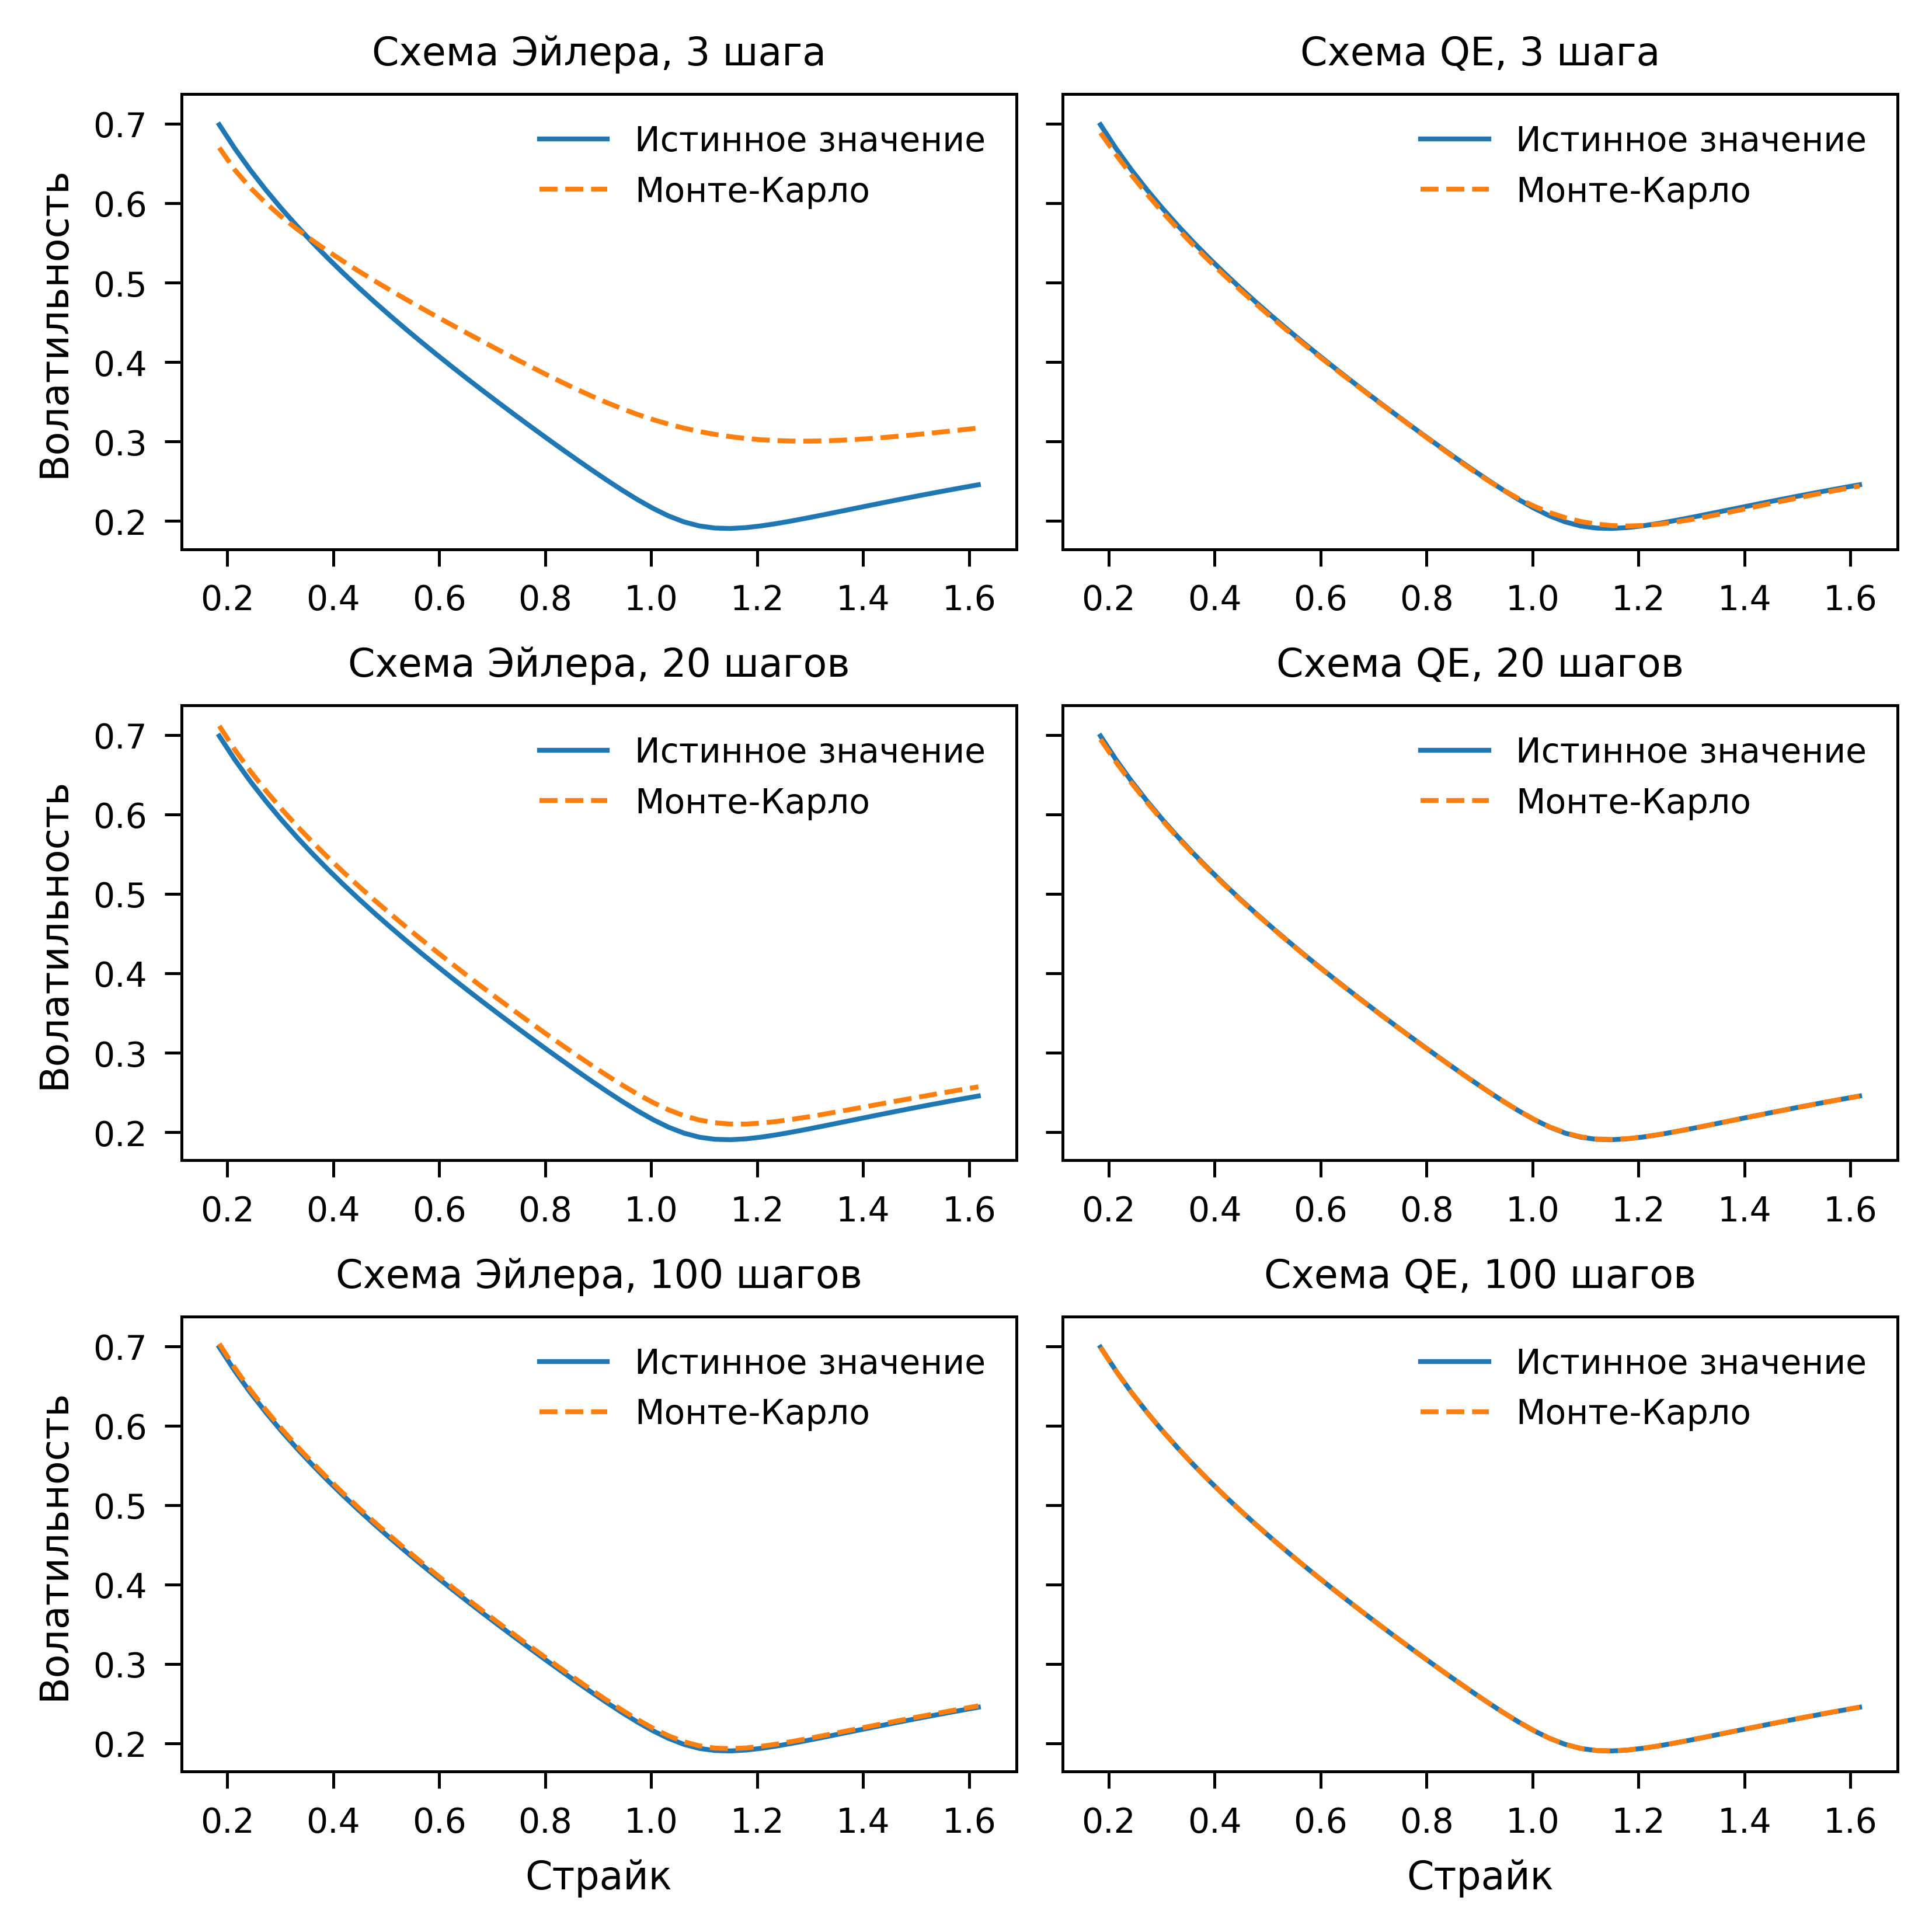
\includegraphics{pic/heston-qe.png}  
\caption{Сравнение точности схемы Эйлера и схемы QE.}
\label{qe:f:comparison}
\end{figure}


\clearpage
\titlecontents{chapter}[0em]{}{}{}{\dotfill\contentspage}
\phantomsection
\addtocontents{toc}{\vspace{1em}}
\chapter*{Список литературы}
\addcontentsline{toc}{chapter}{\textbf{Список литературы}}

\defbibheading{mainbooks}{\section*{Основные источники: книги}}
\defbibheading{mainpapers}{\section*{Основные источники: статьи}}
\defbibheading{aux}{\section*{Дополнительные источники}}
\printbibliography[keyword=fm2-main,heading=mainbooks,type=book]
\printbibliography[keyword=fm2-main,heading=mainpapers,type=article]
\printbibliography[notkeyword=fm2-main,heading=aux]

\end{document}
